\documentclass[11pt,a4paper]{article}
\usepackage[paper=a4paper,width=15cm,height=22cm,twoside]{geometry}

\usepackage{xltxtra}

\usepackage{setspace}
\linespread{1.15}
\setlength{\parskip}{0.75em}
\setlength{\parindent}{0em}

\usepackage{fancyhdr}
\pagestyle{fancy}
\fancyhead{}
\fancyfoot{}
\fancyfoot[RO,LE]{\thepage}
\renewcommand{\headrulewidth}{0pt}
\renewcommand{\footrulewidth}{0pt}

\usepackage[german]{babel}
\usepackage{graphicx}
\usepackage{acronym}

\usepackage{hyperref}
\usepackage[usenames,dvipsnames]{xcolor}
\hypersetup{
    bookmarks=true,
    colorlinks=true,
    linkcolor=NavyBlue,
    citecolor=NavyBlue,
    urlcolor=NavyBlue
}

\bibliographystyle{plain} 
\bibdata{parts/bibliothek} 

\usepackage{sectsty}
\allsectionsfont{\sffamily} 

\usepackage{amsfonts}

\usepackage{multicol}

\begin{document}

\setmainfont[Mapping=tex-text]{ITC Stone Sans Std}

\pagenumbering{roman}

\newcommand{\TODO}{\textcolor{red}{\textbf{TODO}}}
\newcommand{\citequotes}[1]{\textit{„#1“}}
\newcommand{\typoquotes}[1]{»#1«}
\newcommand{\trademark}[1]{\textsf{#1}}

\newcommand{\ball}[1]{\textcircled{\textsf{{\tiny #1}}}}

\definecolor{lightgrey}{RGB}{220,220,220}
\newcommand{\secbar}{\begin{center}{\color{lightgrey}{\rule{0.5\textwidth}{5pt}}}\end{center}}


% Legt Trennungen für Worte fest, die nicht im Wörterburch enthalten sind

\hyphenation{Of-fi-ce}
\hyphenation{Da-tei-en}
\hyphenation{Copy}
\hyphenation{Paste}

\author{Markus Tacker}
\title{Konzeption und Entwurf eines workflowgesteuerten Systems zur Verwaltung von Textbausteinen für Informations- und Kommunikationsmedien}

\begin{center}

\begin{small}

\textbf{Hochschule RheinMain\\Fachbereich Design Informatik Medien\\Studiengang Medieninformatik}

\vspace{1cm}

\textbf{Bachelor-Thesis\\zur Erlangung des akademischen Grades\\Bachelor of Science – B.Sc.}

\end{small}

\vspace{2cm}

\begin{huge}

\textbf{Konzeption und Entwurf eines workflowgesteuerten Systems zur Verwaltung von Textbausteinen für Informations- und Kommunikationsmedien}

\end{huge}

\end{center}

\setmainfont[Mapping=tex-text,BoldFont={Vollkorn-Bold},ItalicFont={Vollkorn-Italic},BoldItalicFont={Vollkorn-Bold Italic}]{Vollkorn}
\setsansfont[Mapping=tex-text]{ITC Stone Sans Std}

\vspace{8cm}

\begin{tabular}{@{}l l}
vorgelegt von & Markus Tacker\\
am & \today\\
& \\
Referent & Prof. Dr. Jörg Berdux\\
Korreferent & Prof. Thomas Steffen
\end{tabular}

\pagebreak

\section*{Erklärung gem. ABPO, Ziff. 6.4.3}

Ich versichere, dass ich die Bachelor-Thesis selbständig verfasst und keine anderen als
die angegebenen Hilfsmittel benutzt habe.

\vspace{1cm}

\begin{tabular*}{\textwidth}{@{\extracolsep{\fill}}l r@{}}
Offenbach am Main, \today & Markus Tacker
\end{tabular*}

\section*{Verbreitung}

Hiermit erkläre ich mein Einverständnis mit den im folgenden aufgeführten
Verbreitungsformen dieser Bachelor-Thesis:

\begin{tabular*}{\textwidth}{@{\extracolsep{\fill}}l r@{}}
Einstellung der Arbeit in die Hochschulbibliothek mit Datenträger: & nein \\
Einstellung der Arbeit in die Hochschulbibliothek ohne Datenträger: & nein \\
Veröffentlichung des Titels der Arbeit im Internet: & ja \\
Veröffentlichung der Arbeit im Internet: & nein
\end{tabular*}

\vspace{1cm}

\begin{tabular*}{\textwidth}{@{\extracolsep{\fill}}l r@{}}
Offenbach am Main, \today & Markus Tacker
\end{tabular*}

\section*{Satz}

Gesetzt mit \LaTeX{} / XeTeX \\
Schrift: ITC Stone Sans\footnote{\url{http://www.stonetypefoundry.com/itcstoneoverview.html}} und Vollkorn\footnote{\url{http://friedrichalthausen.de/?page_id=411}} von Friedrich Althausen

\section*{Diagramme}

Erstellt mit Graphviz\footnote{\url{http://www.graphviz.org/}} und Google Docs\footnote{\url{https://docs.google.com/}}

\vspace{1cm}

\pagebreak

\section*{Ich danke}

Prof. Dr. Jörg Berdux für die Betreuung dieser Bachelor-Thesis und meinem Korreferenten Prof. Thomas Steffen.

Meinen Interviewpartnern

\begin{tabular}{@{}l l}
Arthur Blozyk & \emph{SMTPI - Sales Information and Communication} bei \emph{MAN Truck \& Bus AG}\\
Carsten Fischer & \emph{UX Designer \& Informationsarchitekt} bei \emph{triplesense GmbH}\\
Masanori Fujita & \emph{Business Unit Manager} bei \emph{Zühlke Engineering GmbH}\\
Jorinde Gessner & \emph{Information Manager} bei \emph{Ogilvy \& Mather Deutschland GmbH}\\
Sandra-Charlotte Hildebrandt & \emph{freie Art-Direktorin}\\
Eva Kümml & \emph{Senior Konzept / User Experience} bei \emph{SinnerSchrader Deutschland GmbH}\\
Jan Lochner & \emph{freier Multimedia-Producer}\\
Sebastian Nell & \emph{Director of USE // Connected Products} bei \emph{Scholz \& Volkmer GmbH}\\
Tobias Rudolphi & \emph{Lead Software Architect} bei \emph{Zühlke Engineering GmbH}\\
Markus Rüb & \emph{SMTPI - Sales Information and Communication} bei \emph{MAN Truck \& Bus AG}\\
Torsten Schölzel & \emph{freier Werbetexter}\\
Marc Stenzel & \emph{freier Berater / Senior Projektmanager New Media}
\end{tabular}

Den Professoren am Fachbereich Medieninformatik der Hochschule RheinMain, besonders Prof. Dr. Peter Barth, Prof. Dr. Jörg Berdux und Prof. Dr. Wolfgang Weitz für ihr tägliches Engagement für Lehre und Studenten.

Der Bundesrepublik Deutschland für das Aufstiegsstipendium.

\section*{Widmung}

Ich widme diese Bachelor-Thesis meiner Frau Tanja die mich ermutigt hat, mit dem Studium zu beginnen.

\pagebreak

\section*{Zusammenfassung}

\TODO

Nahezu alle Informations- und Kommunikationsmedien haben eines gemeinsam: sie beinhalten Text. Obwohl viele Personen bei der Erstellung dieser Texte beteiligt sind, werden sie in der Regel in Office-Dokumenten verwaltet, meistens mit Word, bei großen Projekten kommt Excel zu Einsatz. Der Workflow von einem Bearbeiter zum nächsten erfolgt über den Austausch des Office-Dokumentes via E-Mail, Ticketsysteme oder sonstige System zum asynchronen Dateiaustausch wie z.B. Dropbox. Dieser Prozess ist aufwendig und fehleranfällig. Sobald mehrere Personen gleichzeitig an den Texten arbeiten, wird manuelles Eingreifen notwendig um die gemachten Änderungen zusammenzuführen. Aufgrund der Vielzahl der am Text beteiligten Personen sind Office-Dateien ein denkbar schlecht geeignetes Mittel um Texte und ihre Änderungen sauber und nachvollziehbar zu verwalten. Auch das Übertragen von Texten aus Office-Dokumenten ist eine Fehlerquelle – es ist stupides Copy\&\-Paste. In den meisten Fällen müssen dabei im Dokument vorgenommene Formatierungen wie Umbrüche und Absätze entfernt werden um eine saubere Darstellung im Endprodukt zu gewährleisten. Gerade der Text ist der Bestandteil eines Informations- und Kommunikationsmediums, der oft bis zur letzten Minute geändert wird – egal wie viel Aufwand vorher in die Planung geflossen sind. Dies liegt unter anderem daran, dass Text im Gegensatz zu Grafiken, Fotos und anderen Multimedia-Elementen als einziger Informationsträger eindeutig ist und üblicherweise keinen Interpretationsspielraum offen lassen soll. So bietet er auch aus rechtlicher Sicht den problematischsten Bestandteil des Produkts.

Diese Bachelor-Thesis analysiert das beschriebene Problem und konzipiert einen passgenauen Worflow, der alle Beteiligten entsprechend ihrer Aufgabe und Anforderungen integriert. Als Proof-of-Concept wird eine webbasiertes Anwendung entworfen, die den konzipierten Workflow soweit abbildet, dass das Konzept am Beispiel einer Informationsbroschüre überprüft werden kann. 

Im Abschnitt~\ref{l:entwurf} wird eine web-basierte Anwendung entworfen, die diesen Anforderungen entspricht. Im Abschnitt~\ref{l:personas} werden schließlich Personas vorgestellt, die typische Benutzer der Lösung repräsentieren und zur Überprüfung des Konzeptes verwendet werden.

\pagebreak

\pagebreak

\tableofcontents

\pagebreak

\setcounter{page}{1}
\pagenumbering{arabic}

\section{Definition}
\label{l:def}

In dieser Bachelor-Thesis werden bestimmte allgemeine Begriffe und deren Synonyme verwendet, deren konkrete Bedeutung im Kontext dieser Arbeit wie folgt definiert ist:

\paragraph{Workflow (Ablauf)} Allgemein lässt sich sagen, dass ein Workflow aus den zum Erreichen eines Zieles nötigen Arbeitsschritten besteht. \cite[S.8]{wmc} definiert einen Workflow als die Automatisierung eines Business-Prozesses, als Ganzes oder in Teilen, in welchem Dokumente, Informationen oder Aufgaben entsprechend einer Menge von prozeduralen Regeln von einem zum anderen Teilnehmer zur Bearbeitung weitergegeben werden. 

\paragraph{Text (Textbaustein)} Damit sind die kleinsten sinnvoll identifizierbaren Bestandteile gemeint, aus denen sich der Text eines Produktes zusammensetzt. Dies sind in der Regel einzelne Sätze bei Druckmedien, können aber auch einzelne Worte sein, wie z.B. die Beschriftung einer Schaltfläche in einer Anwendung.

\paragraph{Medium (Medien-Produkt, Produkt)} Medien sind physische oder elektronische Informationsträger. Diese Bachelor-Thesis beschäftigt sich vor allem mit Informations- und Kommunikationsmedien und hierbei vor allem mit Massenkommunikationsmitteln, sowohl physischer als auch technischer Natur (vgl. \cite[S.199--201]{schanze2002metzler}). Dies können z.B. Marketingmedien wie Broschüren oder Fernsehwerbespots sein aber auch softwarebasierte Produkte wie eine Smartphone-Anwendung oder eine Internetseite. 

\paragraph{Agentur} Ein Unternehmen das Medien erstellt. In der Regel sind dies Werbeagenturen, Medien-Produktionsfirmen oder Software-Systemhäuser. 

\paragraph{Projekt} Die Erstellung von Medien erfolgt in Agenturen in Projektarbeit. Projekte sind zeitlich begrenzt und vereinen zielgerichtet die zur Erstellung des Produktes beteiligten Mitarbeiter und Ressourcen. 

\paragraph{Kunde} Ein Unternehmen das Agenturen mit der Erstellung von Medien beauftragt.

\paragraph{Nutzer} Eine Person, die ein Medium konsumiert oder ein Produkt verwendet.

\paragraph{Werkzeug (Anwendung)} Eine Software, die eine spezielle Funktion erfüllt. Adobe Photoshop ist ein Werkzeug zur Bearbeitung von Bildern.

\paragraph{Wireframes} Wireframes dienen zur schnellen Skizzierung eines Produktes mit Hilfe von einfachen geometrischen Formen und Texten. Sie werden angefertigt, um einen Überblick über den gesamten Umfang eines Produktes zu bekommen und die wichtigsten Aufgaben zu definieren, die von dessen Nutzern durchgeführt werden.

\paragraph{Ansicht} Bezeichnet eine einzelne Darstellungsvariante in einem Produkt, die sich durch ihre Gestaltung und ihren Aufbau grundlegend von anderen Ansichten unterscheidet.

\pagebreak

\pagebreak

\section{Problem-Analyse}\label{l:problemanalyse}

In diesem Abschnitt werden die Probleme beschrieben, die bei der Erstellung von Informations- und Kommunikationsmedien in Zusammenhang mit den dargestellten Texten auftreten. Abschnitt~\ref{l:besondererolle} analyisiert die besondere Rolle von Text, anschließend zeigt Abschnitt\ref{l:officeprobleme}~(S.\pageref{l:officeprobleme}~ff.) typische Probleme auf, die im Verlauf von Projekten entstehen. Abschnitt~\ref{l:praxisbeispiele}~(S.\pageref{l:praxisbeispiele}~ff.) belegt dies mit Beispielen aus der Praxis. 

Die Analyse des Problems basiert auf Interviews mit Menschen, die in ihrem Arbeitsalltag regelmäßig mit Texten zu tun haben.

\subsection{Die besondere Rolle von Text in Informations- und Kommunikationsmedien}\label{l:besondererolle}

Es existieren nahezu keine Medien, die ohne Texte auskommen, denn Text ist im Gegensatz zu Grafiken, Fotos oder Animationen ein eindeutiger Informationsträger und unterliegt viel weniger stark einer Interpretation durch den Rezipienten eines Mediums als die symbolisierte oder stilisierte Darstellung von Informationen in audiovisuellen Medien. Text wird in der Marketing-Kommunikation als Unterstützung der zu übermittelnden Information verwendet. Hat man die Aufmerksamkeit des Betrachter eines Produkts erlangt, liefert Text weitere Informationen zum Produkt, er dient dazu, die emotionale Botschaft zu erläutern und zu präzisieren. Auch aus rechtlichen Aspekten ist Text aus den genannten Gründen der einzige verbindliche Informationsträger -- bestes Beispiel hierfür ist das sogenannte \typoquotes{Kleingedruckte}, dass sich gerade bei inhaltlich sehr stark komprimierten Werbeformen, wie z.B. Plakat- oder Fernsehwerbung, findet. Ist die Textmenge, die in der Marketing-Kommunikation zum Einsatz kommt, noch überschaubar, gibt es doch Medien die hauptsächlich aus Text bestehen. Hierunter fallen klassische Druckerzeugnisse wie Broschüren und Kataloge oder Produkte der Unternehmenskommunikation wie Jahresberichte und Pressemeldungen. Besonders digitale Medien werden oft mit großen Textmengen versehen -- von der einfachen Produkt-Microsite, über Werbemittel wie Newsletter bis zur Unternehmenswebsite -- die Möglichkeit Inhalte hierarchisch zu strukturieren und sogar über eine Suche zugänglich zu machen hebt eine Limitierung des Umfanges, wie bei Druckprodukten, praktisch auf.

\begin{figure}[htb]
\begin{center}
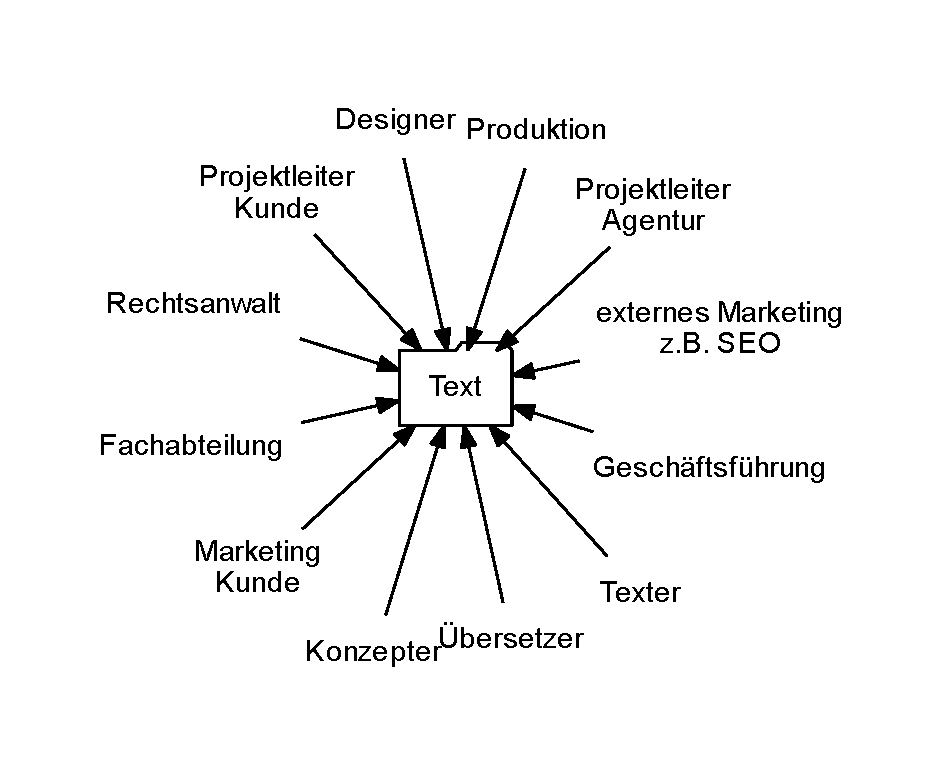
\includegraphics[width=\textwidth]{media/chart-2.pdf}
\end{center}
\caption{Bei der Erstellung von Texten beteiligte Personen}
\label{chart:2}
\end{figure}

Betrachtet man die Abläufe von Projekten, in deren Verlauf Medien erstellt werden, lassen sich bezüglich der Textbestandteile dieser Produkte immer wieder sehr ähnliche Vorgehensweisen und Besonderheiten beobachten. Aufgrund der verbindlichen Natur von Text sind an der Erstellung der Texte für das Medium mehr Personen beteiligt, als es z.B. für die Gestaltung, der Auswahl von Bildmaterial oder für die Programmierung der Fall ist,  da er sehr viele verschieden Kriterien erfüllen muss. Tabelle~\ref{table:textkriterien}~(S.\pageref{table:textkriterien}) listet exemplarisch eine typische Gruppe von Personen auf, die im Verlauf eines Projektes Einfluss auf den Text eines Produktes haben. Dieser Einfluss wird dabei in der Regel nicht in einer sinnvollen Reihenfolge und im Sinne des geplanten Projektverlaufes ausgeübt. Gerade auf die Mitarbeiter auf Kundenseite haben Agenturen keinen Einfluss; in Projektplänen lassen sich zwar verbindliche Termine für die Lieferung von Texten des Kunden festlegen, dies verhindert aber keinesfalls, dass zu einem späteren Zeitpunkt Änderungen notwendig werden -- Hinweise von Anwälten sollten im besten Fall \emph{vor} einer Übersetzung vorliegen, richtet sich aber nach ihren eigenen Terminplänen. Auch die Kriterien wie Text beeinflusst wird, sind sehr vielfältig: Im Entwurf und in der Umsetzung der Produkte legen Designer, Architekten und Produzenten die Struktur von Text wie Art der Ansprache, maximale Wortlänge, Anzahl der Wörter einer Überschrift fest oder diese werden durch das verwendete Medium vorgegeben, Texter legen die Inhalte fest, die wiederum durch Wünsche des Kunden beeinflusst werden; das Lektorat, Fachabteilungen und Anwälte begutachten die Texte dann bezüglich der jeweils erforderlichen Korrektheit.

\begin{table}
\begin{center}
\begin{tabular}{@{}l l l l}
\textbf{Kriterium} & \textbf{Art} & \textbf{Verantwortlich} & \textbf{Organisation}\\
\hline
Aufgabenverteilung & Mitarbeiter & Projektleiter & Agentur\\
\hline
Zielgruppe & Struktur & Informationsarchitektur & Agentur\\
\hline
Umfang, Satzlänge & Struktur & Art-Direktion & Agentur\\
\hline
Länge einzelner Wörter & Struktur & Programmierer & Agentur\\
\hline
Information & Inhalt & Texter & Extern\\
\hline
Orthographie & Korrektheit & Lektorat & Extern\\
\hline
Übersetzung & Sprache & Übersetzungsbüro & Extern\\
\hline
Suchmaschinen-Optimierung & Inhalt & SEO-Experte & Extern\\
\hline
Aufgabenverteilung & Mitarbeiter & Projektleiter & Kunde\\
\hline
Fachliche Aspekte & Korrektheit & Fachabteilung & Kunde\\
\hline
Rechtliche Aspekte & Korrektheit & Rechtsanwalt & Kunde\\
\hline
Werbeaussagen & Inhalt & Marketingabteilung & Kunde\\
\hline
… & … & …
\end{tabular}
\caption{Kriteren von Textbausteinen und verantwortliche Personen}
\label{table:textkriterien}
\end{center}
\end{table}

Wie man Tabelle~\ref{table:textkriterien}~(S.\pageref{table:textkriterien}) entnehmen kann, existieren vielfältige Einflussmöglichkeiten auf die Gestaltung von Texten für Medien die sich auf viele Verantwortliche verteilen. Der Grund dafür ist, dass alle Beteiligten jeweils spezifisches Fachwissen in den Text einfließen lassen, seien es gestalterische Aspekte, die Einfluss auf die Struktur haben, oder das wissen über exakte technische Abläufe, die nur Spezialisten in den Fachabteilungen auf Kundenseite bekannt sind. Dieses Expertenwissen kann nicht für die meist kurze Projektlaufzeit an die umsetzenden Agentur vermittelt werden. Es ist also unvermeidlich, dass Text während des gesamten Projektverlauf geändert werden kann. Neben den Einflüssen durch Experten gibt es auch projektbedingte Einflüsse auf Text in letzter Minute. Sind in Texten Informationen enthalten sind, die einen zeitlichen Aspekt abbilden, ergeben sich durch Verzögerungen im Projekt automatisch Änderungsanforderungen. Ein Beispiel sind Gewinnspiele: Verschiebt sich durch Probleme während dem Projekt der Zeitpunkt, ab dem ein Produkt beim Rezipienten vorliegt, müssen auch eventuell knapp kalkulierte Gewinnspieltermine angepasst werden. Ein weiterer Grund für vielfältige Textänderungen im Verlauf eines Projektes ist die Erwartungshaltung des Kunden -- da es Kunden aus ihrem eigenen Arbeitsalltag gewöhnt sind, mit Textverarbeitungsprogramme zu arbeiten, und sie so aus eigener Erfahrung vermeintlich wissen dass Texte schnell geändert sind, erwarten sie auch, dass die Texte im Produkt bis zum Schluss geändert werden können; ihnen ist nicht bewusst, das vom ursprünglichen Text im Quelldokument bis zur Darstellung im fertigen Produkt viele aufwändige Arbeitsschritte nötig sein können.

\bigskip

In diesem Abschnitt wurde gezeigt, das Texte in Medien durch viele Personen und über den gesamten Verlauf eines Projektes geändert werden können. Im nächsten Abschnitt wird erläutert, wie der Austausch über diese Textänderungen erfolgt und welche Probleme dabei entstehen.

\subsection{Das Werkzeug der Wahl zur Verwaltung von Text: Textverarbeitungs- und Tabellenkalkulationsprogramme}

Zur Abbildung der komplexen Abläufe bei der Erstellung von Informations- und Kommunikationsmedien liefern etablierte Software-Hersteller passende Lösungen auch speziell für Texte: Mit \emph{InCopy} liefert \emph{Adobe} eine \typoquotes{Lösung für Texterstellung und -bearbeitung, die aufgrund der engen Integration mit Adobe InDesign® CS5.5 effektivere Zusammenarbeit zwischen Redakteuren und Layoutern ermöglicht} \cite{adobeincopy} und  die \emph{Content Station} von \emph{Woodwing} \typoquotes{ist […] eine einzige Oberfläche für alle Schritte des Publishing-Prozesses. […] Unter Nutzung der Desktop- oder der Web-Version können die Team-Mitglieder unabhängig ihres Aufenthaltsorts mitarbeiten} \cite{woodwing} -- um nur zwei Beispiele zu nennen. Doch obwohl spezialisierte Werkzeuge existieren findet man diese in Agenturen nur selten -- das Werkzeug der Wahl zur Verwaltung der Texte ist in der Regel eine in der Agentur vorhandene Textverarbeitungs- oder Tabellenkalkulationssoftware, in den allermeisten Fällen handelt es sich dabei um den Marktführer in diesem Bereich: \emph{Microsoft} \emph{Word} oder \emph{Excel}. Auf die Probleme, die durch deren Einsatz entstehen wird im nachfolgenden Abschnitt~\ref{l:officeprobleme}~(S.\pageref{l:officeprobleme}) eingegangen. Zu erst muss jedoch erst untersucht werden, warum \emph{Word} oder \emph{Excel} statt spezieller Werkzeuge eingesetzt werden, die für den komplizierten Workflow in Projekten entwickelt wurden. 

Oberflächlich betrachtet, bieten Textverarbeitungsprogramme die notwendigen Funktionen, um Texte zu verwalten und sind damit scheinbar die natürliche Wahl. Die verwendeten Funktionen sind dabei nachfolgend beschrieben.

\begin{figure}[htb]
\begin{center}
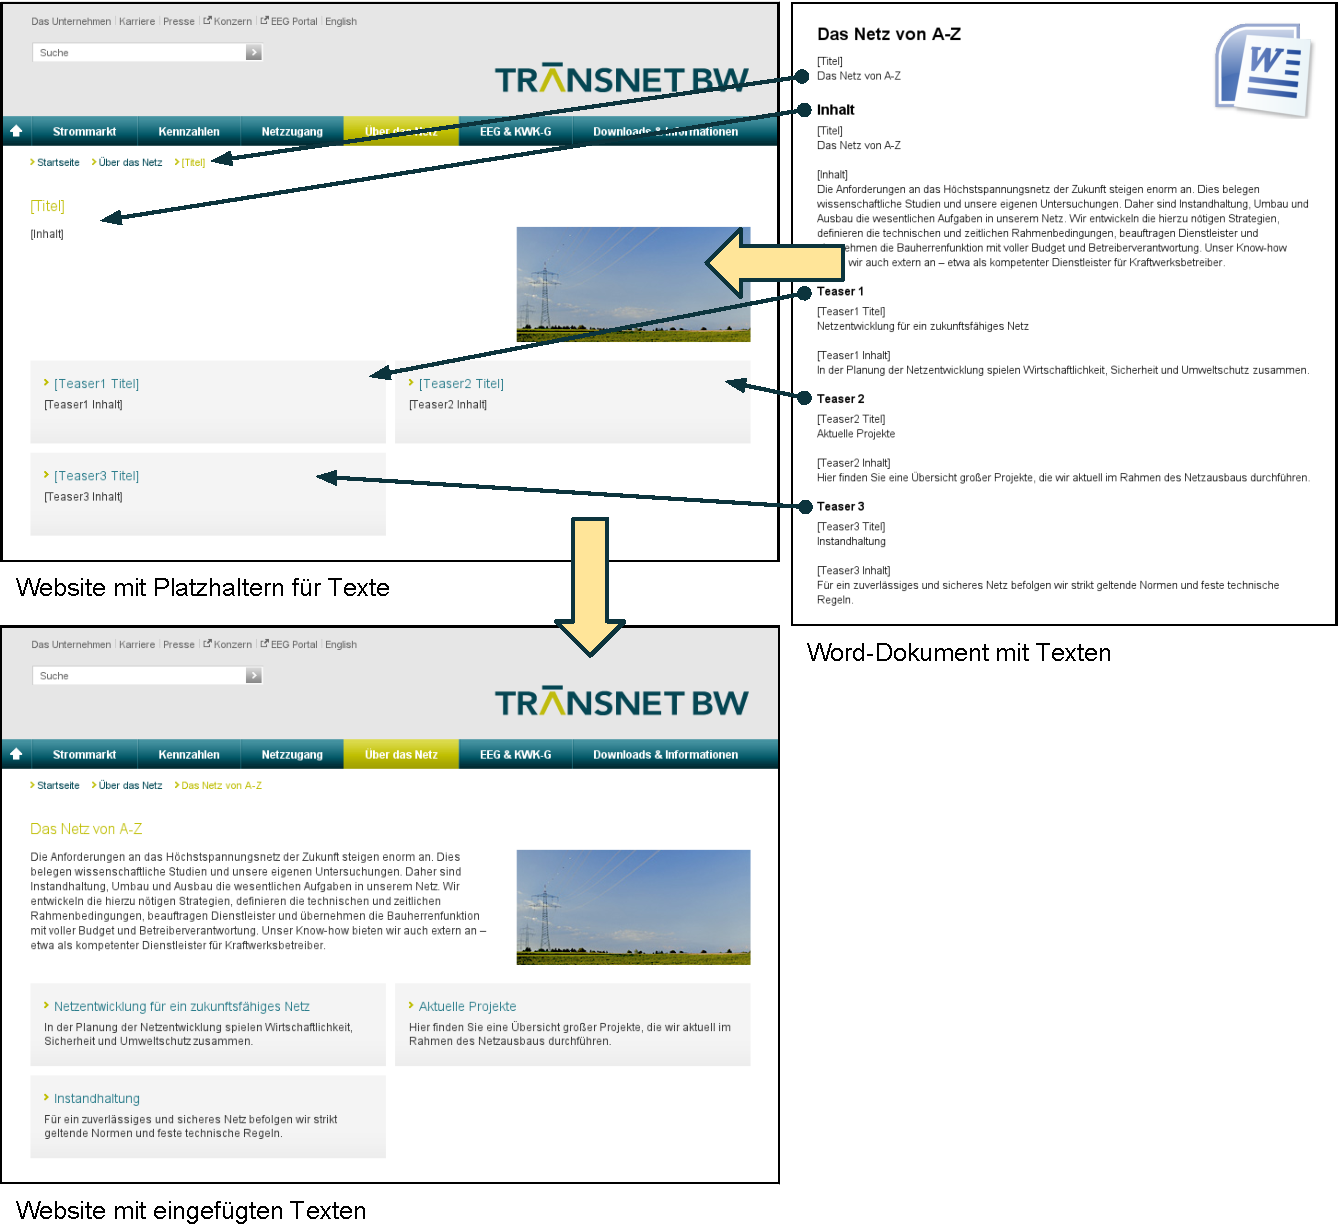
\includegraphics[width=\textwidth]{media/Textbooklet-Word-Dokument.pdf}
\end{center}
\caption{\emph{Word}-Dokument mit Texten für eine Internetseite}
\label{f:wordbooklet}
\end{figure}

\begin{figure}[htb]
\begin{center}
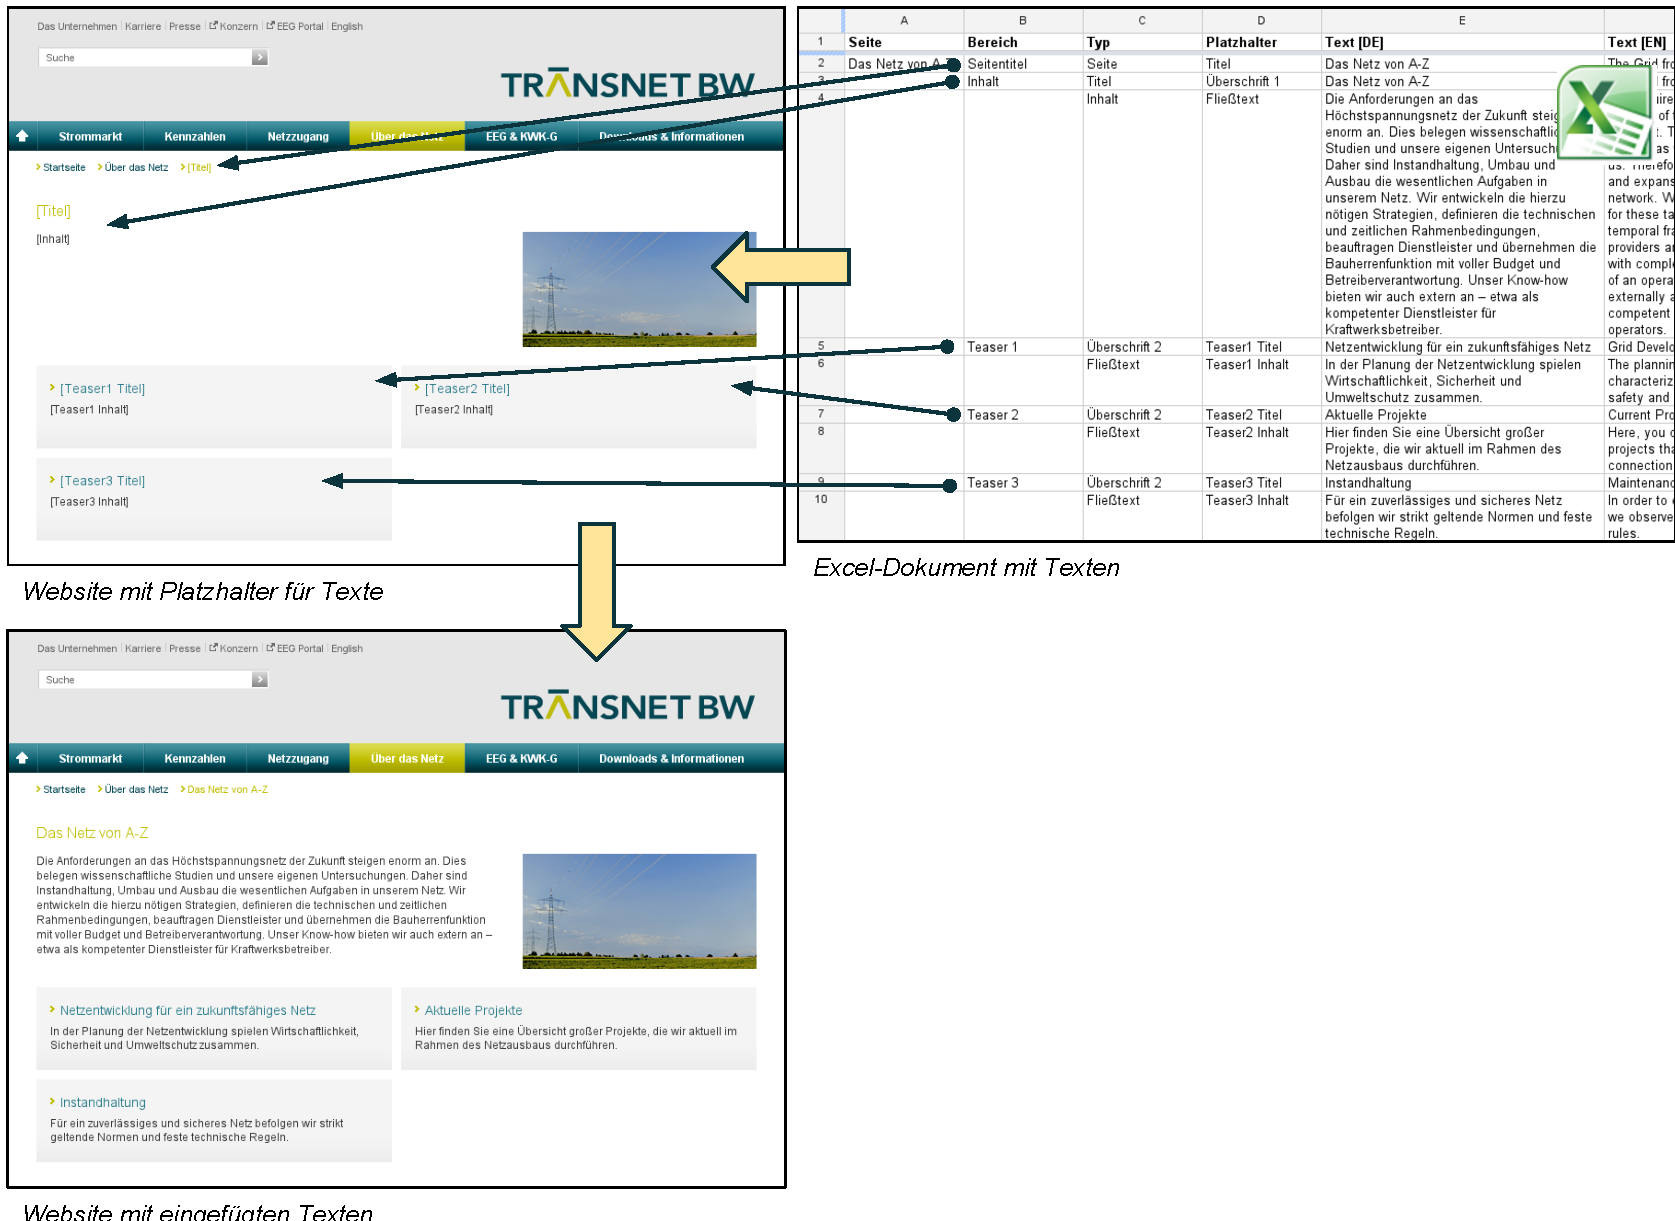
\includegraphics[width=\textwidth]{media/Textbooklet-Excel-Dokument.pdf}
\end{center}
\caption{\emph{Excel}-Dokument mit Texten für eine Internetseite}
\label{f:excelbooklet}
\end{figure}

\paragraph{Strukturierung von Texten} Die Möglichkeit, Texte hierarchisch in Dokumente, Seiten, Kapitel, Abschnitte oder Absätze zu unterteilen ermöglicht es die Textbausteine für ein Produkt geordnet zu Erfassen. Neben den eigentlichen Texten lassen sich dazu auch Zusatzinformationen wie den Typ des Textes
(vgl. Abschnitt~\ref{l:textattribute},~S.\pageref{l:textattribute}) dort zuzuordnen. Abbildung~\ref{f:wordbooklet}~(S.\pageref{f:wordbooklet}) zeigt beispielhaft ein \emph{Word}-Dokument, in dem die Texte für eine Website definiert werden. Im Dokument existiert pro Seite der Internetpräsenz jeweils ein Abschnitt, der alle Texte auf der Seite beschreibt. Dort finden sich die Texte zu den Platzhaltern, die in der Website verwendet werden, die dann an deren Stelle eingefügt werden. Über die Formatierung der Überschriften wird die Hierarchie der Texte definiert. Die Verwendung von Tabellen statt Dokumenten ist eine weitere Möglichkeit die verwendeten Texte zu erfassen. Abbildung~\ref{f:excelbooklet}~(S.\pageref{f:excelbooklet}) zeigt beispielhaft ein \emph{Excel}-Dokument, in dem pro Zeile ein Text definiert wird. In den Spalten findet sich neben dem eigentlichen Text Zusatzinformationen wie Informationen zum Typ. Tabellarische Dokumente werden oft bei umfangreichen Projekten verwendet, oder um mehrere Sprachversionen zu verwalten.

\paragraph{Rechtschreibkorrektur} In Textverarbeitungsprogrammen sind ausgefeilte Funktionen zur Rechtschreibkorrektur enthalten, die bereits während der Eingabe auf Fehler aufmerksam machen und für viele Sprache integriert sind. So ist sichergestellt, dass bereits die erste Version eines Textes relativ wenige Fehler enthält.

\paragraph{Kommentare} Es ist möglich, in \emph{Word}- und \emph{Excel}-Dokumenten Kommentare zu hinterlassen. Diese werden gesondert hervorgehoben und können zum Austausch über den Text oder für Hinweise zur Verwendung hinterlegt werden und von allen Bearbeitern eingesehen werden.

\paragraph{Änderungsverfolgung} Wenn die Änderungsverfolgung aktiviert ist, werden alle Änderungen an einem Dokument aufgezeichnet. Diese Information kann dazu verwendet werden, um mehrere Versionen eines Dokumentes zusammenzuführen oder Änderungen an Inhalten vorzuschlagen, zu prüfen und selektiv zu übernehmen.

\paragraph{Verzeichnisse} In \emph{Word}-Dokumenten ist es möglich, Verzeichnisse wie z.B. ein Inhaltsverzeichnis anzulegen. Dies hilft dabei, bei größeren Projekten einen Überblick über den Aufbau des Produktes zu erhalten, sofern die Inhalte mit den passenden Formatvorlagen versehen wurden.

\paragraph{Suchen \& Ersetzen} Da sich die Texte in einem großen Dokument befinden können mit den Funktionen zum Suchen \& Ersetzen schnell bestimmte Inhalte gefunden und angepasst werden.

\paragraph{Export} Die \emph{Office}-Programme verfügen über die Möglichkeit des Exports in verschiedene Formate. Verwendet werden vor allem PDF bei \emph{Word}-Dokument zur Abstimmung, unter andere auch deswegen, weil es in \emph{Adobe} \emph{Acrobat} umfangreiche Korrekturfunktionen gibt, und CSV in \emph{Excel}, das möglich macht die Text mit Hilfe von speziellen Programmen in andere Systeme zu importieren.

\paragraph{Formatierungsfunktionen} Mit umfangreiche Formatierungsfunktion ermöglichen zusätzliche Informationen zu Texten zu hinterlegen. Oft werden durch farbige Markierung Passagen markiert, die zu überarbeiten sind, entfallen oder inhaltlich überarbeitet werden müssen. Auch können Formatieren so angelegt sein, dass sie in das Produkt übernommen werden sollen -- in der Regel werden dann Teile des oder einzelne Wörter Textes fett oder kursiv formatiert. Funktionen zum Setzen von Hyperlinks werden gerade bei Web-Projekten verwendet um Links zu definieren, die im Produkt verwendet werden sollen.

\bigskip

Auch im Hinblick auf nicht-funktionale Aspekte bieten Textverarbeitungsprogramme einige Vorteile, sind sie doch in den allermeisten Unternehmen der Standard zur Textverarbeitung und sogar plattformunabhängig verfügbar -- zumindest existiert die Möglichkeit das \emph{Microsoft Office}-Dateiformat auf allen Plattformen zu bearbeiten. Da bei allen Projektbeteiligten eine Installation von \emph{Microsoft Office} vorausgesetzt werden kann, werden \emph{Word} und \emph{Excel} zu \typoquotes{leichtgewichtigen} Werkzeugen, das vom vom Anwender keine zusätzlichen Aufwände, z.B. bei der Installation oder Eingewöhnung, abverlangen. Selbst auf Plattformen die von \emph{Microsoft Office} nicht offiziell unterstützt werden, wie z.B. Linux, existieren Programme mit denen das Office-Dokumenten-Format geöffnet und bearbeitet werden kann, unter Linux ist dies z.B. \emph{Libre Office}. Da \emph{Office}-Dokumente in nur einer Datei gespeichert werden, sind diese einfach auszutauschen -- in Agenturen werden die Dateien in der Regel auf einem Netzwerk-Laufwerk gespeichert, unternehmensfremde Mitarbeiter erhalten die Dateien via E-Mail, FTP-Server oder Filesharing-Anbieter, z.B. Dropbox. So wird das gemeinsame Arbeiten an den Texten, zumindest nacheinander, möglich. 

\bigskip

Wie in diesem Abschnitt gezeigt wurde, sind Textverarbeitungs- und Tabellenkalkulationsprogramme wie \emph{Microsoft} \emph{Word} und \emph{Excel} nominell für den Einsatz zur Verwaltung von Texten für Medien geeignet. Dies erklärt, warum sie zu Beginn eines Projektes als geeignet angesehen und in Agenturen immer wieder als Werkzeug für die Erfassung, Definition und Übersetzung der Texte eines Projektes ausgewählt werden. Im alltäglichen Gebrauch treten jedoch Probleme gerade im Bereich des gemeinsamen Bearbeitens, paralleler oder nachträglicher Änderungen und der Übertragung der fertigen Texte in den Produktionsprozess auf, die im folgenden Abschnitt erläutert werden.

\subsection{Probleme bei der Verwendung von Textverarbeitungs- und Tabellenkalkulationsprogrammen im Verlauf eines Projektes}
\label{l:officeprobleme}

Wie im vorangegangenen Abschnitt gezeigt wurde, sind Textverarbeitungs- und Tabellenkalkulationsprogramme wie \emph{Microsoft} \emph{Word} und \emph{Excel} der Standard für die Verwaltung von Texten in Projekten zur Erstellung für Informations- und Kommunikationsmedien. In den für diese Bachelor-Thesis geführten Interviews haben jedoch alle Personen von vielfältige Problemen in Zusammenhang mit diesen Programmen berichtet. Dies belegt zum einen, dass am gängigen Workflow viele Möglichkeiten zur Verbesserung existieren und liefert zum andere auch Hinweise, wie der verbesserte Workflow im Detail gestaltet werden muss. In diesem Abschnitt werden die beobachteten Probleme beschrieben.

\label{p:serielles-konzept}\paragraph{Serielles Bearbeitungskonzept} Das grundsätzliche Bearbeitungskonzept, das in \emph{Word} und \emph{Excel} zum Einsatz kommt ist seriell, das bedeutet, dass eine Dokument gleichzeitig nur von einer Person bearbeitet werden kann. Soll mit mehreren Personen an einem Dokument gearbeitet werden, muss dieses zwischen allen Beteiligten ausgetauscht werden. Dies geschieht, in dem die Dokumenten-Datei entweder per E-Mail jeweils zum nächsten Bearbeiter verschickt wird oder die Datei auf ein, durch alle Beteiligten erreichbaren Speicherplatz verschoben werden. In Agenturen handelt es sich hierbei meistens um eine Netzwerklaufwerk -- hierauf haben aber nur die im lokalen Netzwerk integrierten Mitarbeiter Zugriff. Soll die Datei auch externen Mitarbeitern oder dem Kunden zur Verfügung gestellt werden, werden diese wieder per E-Mail verschickt oder in extern erreichbare Speicherort kopiert, wie z.B. FTP-Server, Wikis und Extranet-Portale oder es kommen spezielle Programme zum Dateiaustausch zum Einsatz, wie z.B. \emph{Dropbox}. Die Organisation dieses Austausches ist besonders dann aufwändig, wenn Dateien sich nicht mehr unter Kontrolle der Agentur befinden, weil sie z.B. zum Kunden zur Kontrolle geschickt wurden. Dann kommt es dazu, dass mehrere Versionen des Dokumentes parallel existieren: eine Version beim Kunden, die dort mit Änderungen und Ergänzungen versehen wird und eine Version in der Agentur in der sich aufgrund von Änderungen im Verlauf des Projekts Text ändern. Um anschließend alle Beteiligten auf den aktuellen Stand zu müssen die verschiedenen Versionen des Dokumentes manuell zusammengeführt werden -- automatisiert ist das mit \emph{Word} und \emph{Excel} nicht möglich. Neben dem zeitlichen Aufwand birgt das manuelle Zusammenführen weitere Fehlerquellen, da Änderungen an Texten durch Copy\&Paste übertragen werden, kann es gerade bei großen Dokumenten passieren, dass man die Änderungen an der falschen Stelle einarbeitet, sofern im Dokument sich ähnelnde Textabschnitte existieren. Aus Kostengründen und weil es sich dabei um eine repetitive Arbeit handelt ist es nicht selten der Fall, dass diese Änderungen von Praktikanten oder studentischen Aushilfen durchgeführt werden, die mangels inhaltlicher Kenntnis den Zusammenhang der Text nicht kennen, was ebenfalls die irrtümliche Änderungen am Text durch fehlerhaftes Copy\&Paste begünstigt. Auch ist die Eindeutigkeit der Dateiversionen nicht gewährleistet, allein aufgrund des Zeitstempels kann keine genaue Aussage darüber getroffen werden, welche Datei die neueste ist. So muss man sich auf ein Benamungsschema für Dateien einigen, das im besten Fall klar erkennen lässt \emph{welches} Dokument das neueste ist. Üblich sind dabei Ergänzungen des Dateinamens mit Datumsinformationen, wie z.B. \texttt{Text\_Online\_2012-04-13.docx}. Folgen nicht alle Beteiligten diesem Schema, weil diese z.B. nicht ausreichend informiert sind, oder kommt es zu gleichzeitiger Änderungen von zwei Personen kann es so auch zu zwei verschiedenen Dateien mit dem gleichen Dateinamen kommen. Durch die Verteilung der Dokumente an verschiedene Speicherorte kommt es zu Situationen, in denen nicht klar ist, wer aktuell die \emph{neueste} Dateiversion hat. 

Tatsächlich existiert mit dem \emph{Microsoft} \emph{SharePoint}, einer Software für Intra-, Extra- und Internetportale, eine Lösung, die diese Probleme behebt \cite{sharepoint-shared-documents}. Mit Hilfe von \emph{Shared Documents} lassen sich Dokument zentral ablegen. Sollen diese editiert werden, müssen Sie von der jeweiligen Person \typoquotes{ausgecheckt} werden, dies sperrt den Zugriff auf das Dokument durch andere Mitarbeiter. Sobald das Bearbeiten abgeschlossen wurde, wird die Datei wieder \typoquotes{eingecheckt}. So wird sichergestellt, dass es nie zwei Versionen der Datei mit unterschiedlichen Änderungen gibt. Diese Funktion behebt aber nicht den Umstand, das an einem Dokument immer nur eine Person arbeiten kann. Des weiteren ist \emph{SharePoint} im Agentur-Umfeld kaum anzutreffen, was dem Umstand geschuldet ist, dass der Betrieb einer \emph{SharePoint}-Instanz mit hohen Lizenz- und Personalkosten verbunden ist. Zum anderen setzen die Funktionen zum gemeinsamen Bearbeiten von \emph{Word} oder \emph{Excel} voraus, dass alle Mitarbeiter über die neuesten Version verfügen \cite{sharepoint-wordversions}. Dies kann aber auf Kundenseite nicht vorausgesetzt werden. Aufgrund der unterschiedlichen Programm-Versionen aber auch unterschiedlicher Betriebssystemen, kommt es beim Austausch der Dateien zu verschiedenen Kompatibilitätsproblemen, da in Agenturen meistens \emph{Mac OS} verwendet wird, auf Kundenseite jedoch \emph{Windows} verbreitet ist.

\paragraph{Monolithische Dokumente} Das Zusammenführen aller Textbausteine eines Produktes in einem Dokument hat den Nachteil, dass diese nur als Ganzes weitergeben werden können. In bestimmten Konstellationen ist es aber notwendig, sicherzustellen, dass bestimmte Inhalte nicht von allen Projektbeteiligten einsehbar sind. Zum einen kann es sich dabei um Informationen handeln, die der Geheimhaltung unterliegen oder sensibel sind, so dass sie nur bestimmten Personen zugänglich sein dürfen. Zum anderen kann es aus Kostengründen sinnvoll sein, die Prüfung von Texten durch Anwälte, oder die Übersetzung von Texten auf bestimmte Bereiche einzuschränken. In diesen Fällen wird es notwendig, verschieden Versionen des Dokumentes anzulegen, die an den jeweiligen Personenkreis angepasst sind. Dies erzeugt die Problem, die im vorangegangenen Abschnitt beschrieben wurden.

\paragraph{Feedback} Durch das Verteilen der Dokumente auf verschiedenen Speicherorten wird eine parallele Kommunikation des Arbeitsstandes mittels E-Mail nötig, bei der jeweils dem nächsten Bearbeiter mitgeteilt wird, dass er mit seiner Aufgabe weiter fortfahren kann. Der Ablauf und die Reihenfolge der Kommunikation ergibt sich durch die Aufgaben der Betiligten Personen, aber auch durch informelle Absprachen. Gerade zwischen Agentur und Kunden gibt es häufig \typoquotes{Flaschenhälse}, die zu Verzögerungen führen. Dies sind in den meisten Fällen die jeweiligen Projektleiter und Ansprechpartner, die auch bei technischen oder inhaltlichen Fragen jeweils der alleinige Empfänger sind, die Anfrage entgegen nehmen in in ihrem Unternehmen an die zuständige Person weiterleiten, auf deren Antwort warten um dann die Antwort zurück zu spielen. Hierdurch bilden sich umfangreiche und langlebige E-Mail-Kommunikationsketten, an denen viele, meistens zu viele, Personen beteiligt sind und in ungeordneter Reihenfolge Feedback liefern.

\paragraph{Strukturierung von Dokumenten} Eine der Gründe, warum \emph{Word} und \emph{Excel} zur Standardausstattung auf jedem Büro-Computer gehören, ist der, dass sie für einen sehr breiten Anwendungsbereich entwickelt wurden. Dies hat jedoch zur Folge, dass es mit einigem Aufwand verbunden ist, die passende Struktur für die Inhalte eines Produktes in einem Text- oder Tabellen-Dokument an zu legen. Hierbei wird meistens eine hierarchische Struktur mit Hilfe von Abschnitten angelegt (vgl. Abbildung~\ref{f:wordbooklet},~S.\pageref{f:wordbooklet}). In \emph{Excel} wird im Hinblick auf die kompaktere Darstellung meisten aus besonderer Formatierungen verzichtet und mit sich wiederholenden Zellen gearbeitet (vgl. Abbildung~\ref{f:excelbooklet},~S.\pageref{f:excelbooklet}), die eine hierarchische Struktur simulieren -- die zweidimensionale Tabellendarstellung ist für komplexere Hierarchien nicht ausgelegt. Dies aufwändige Strukturierung des Dokuments muss auch geschehen, damit sich alle Anwender in den Dokumenten zurecht finden und eine eindeutige Zuordnung zwischen Textbausteinen im Dokument und den dafür vorgesehen Platzhaltern im fertigen Produkt möglich ist. Da beide Programme für diese Aufgabe keinerlei Vorlage und Unterstützung liefern, muss hier viel Arbeit investiert werden, die zudem noch vorausschauend genug sein muss, damit es im späteren Verlauf des Projektes durch nicht berücksichtige Fälle nicht notwendig wird, das Dokument komplett zu überarbeiten.

\paragraph{Formatierung} Die Formatierung der Textbausteine nach gestalterischen Aspekten, also das Hinzufügen von z.B. Hervorhebungen, Unterstreichungen und Absätzen wird zum Teil schon während der Erstellung der Texte vorgenommen. Hierbei werden die jeweiligen Funktionen der von \emph{Word} und \emph{Excel} verwendet. Ist dies in \emph{Word} komfortabel möglich, sind die Möglichkeiten in \emph{Excel} deutlich eingeschränkt. Hier lassen sich Zeichen-Formatierungen wie Hervorhebung, Farbe ö.ä. nicht auf einzelne Worte oder Zeichen anwenden, sondern nur auf eine ganze Zelle. Auch Zeilenumbrüche stellen ein Problem dar. Diese sind zwar grundsätzlich möglich, jedoch kann es mangels Wissen dazu kommen, dass ein Bearbeiter einen Zeilenumbruch nicht innerhalb einer Zelle einfügt, sondern statt dessen eine neue Zeile einfügt. Werden die Zeilennummern oder bestimmte Spalten als Referenz-Schlüssel für den Text verwendet, führt das dazu, dass die zweite Zeile des Texte, nicht mehr zugeordnet werden kann um im Produkt fehlt. Werden Tabellen in \emph{Word}-Dokumenten verwendet um z.B. tabellarische Inhalte in einem Produkt zu beschreiben, führt die aufgrund der beschränkten Seitengröße eines Textdokuments dazu, dass Tabellen mit vielen Spalten nur mit sehr kleinem Text dargestellt werden können, was das Bearbeiten der Texte schwierig macht. Üblich ist auch das Einfügen von Bildern, dies ist nötig, um die Zuordnung der Texte zu Produkten zu erleichtern oder um Untertitel Fotos zu definieren, hierbei treten dann zusätzliche Formatierungsproblem auf, da das platzieren von Bildern nur in beschränktem Maße beeinflusst werden kann. Problematisch ist auch der Austausch der Formatierungen zwischen verschieden Versionen von \emph{Word} oder \emph{Excel}, besonders wenn Dokumente von neueren Versionen in älteren Versionen angezeigt und bearbeitet werden, und vor allem dann, wenn die Dokumente in anderen Textverarbeitungs- und Tabellenkalkulationsprogramm wie z.B. \emph{Apple} \emph{iWorks} oder \emph{LibreOffice} bearbeitet werden. Diese Programme unterstützen zwar \emph{per se} den Ex- und Import von \emph{Microsoft}-Dateiformaten, bei der Konvertierung entstehen gerade bei Übertragen dieser Formatierungen  Unsauberkeiten. Sollen die Formatierungen dann in das Produkt übernommen werden kann dies nicht automatisch geschehen, da es für die verwendete Auszeichnungen keinen Standard gibt, der in allen Umgebungen verwendet werden kann. Deswegen müssen alle Formatierung manuell im Produkt angelegt werden, dies kann, ähnlich wie bei Copy\&Paste, zu Übertragungsfehlern führen.

\paragraph{Feedback und Kommunikation} Neben den eigentlichen Textbausteinen werden in \emph{Word}- und \emph{Excel}-Dokumenten auch Hinweise und Kommentare zu den Texten mit Hilfe von Notizen oder direkt in das Dokument platzierten, besonders formatierten Texten hinterlegt. Werden Notizen verwendet besteht zum einen das Problem, dass diese an einer spezifischen Stelle im Text platziert werden, wird diese Stelle gelöscht, wird damit auch die Notiz ohne einen Warnhinweis gelöscht. Bei der gleichzeitigen Darstellung der Notizen in Kombination mit der Anzeige von Änderungen durch andere Bearbeiter kann das Dokument sehr unübersichtlich werden. Werden Hinweise als Text im Dokument hinterlegt kann diese dazu führen, dass diese Hinweise übersehen werden, oder beim Copy\&Paste von großen Abschnitten unbeabsichtigt in das Produkt übernommen  werden. Diese Unzulänglichkeiten führen dazu dass Feedback auch parallel zu den Dokumenten ausgetauscht wird, meistens mit Hilfe von E-Mails in denen die Anmerkungen bzw. Änderungswünsche aufgezählt werden. Bei der Übersetzung von Texten kommt es mitunter vor, dass Hinweistexte, die zur z.B. Abschnitte kennzeichnen, übersetzt werden, da extern beauftragte Übersetzer sich mit den verwendeten Dokumentenvorlagen nicht auskennen. So werden dann auch beschreibende Texte wie \typoquotes{Überschrift:} übersetzt, was zur Folge hat, dass das Dokument gänzlich unleserlich wird. Übersetzer erhalten auch oft nicht wichtige Zusatzinformationen zu Texten, wie z.B. Angaben über maximale Satzlängen, da sie die fertige abgenommenen Texte in der Ausgangssprache in einem eigenen Dokument erhalten und bei der Erstellung des Dokuments diese, vermeintlich \emph{internen} Hinweise, oft nicht mit übernommen werden.
Informationen darüber, welche Teile zuletzt geändert wurden, können in \emph{Word} und \emph{Excel} zwar aufgezeichnet werden, diese Funktion muss aber Explizit vom Überarbeiter aktiviert werden. Wird dies versäumt kommt es dazu, das Änderungen manuell durch Vergleichen von zwei Dokumenten-Version identifiziert werden müssen, wenn es nicht sinnvoll ist, alle Texte eines Produktes noch einmal zu ersetzen.

\paragraph{Usabilty-, technische und typografische Probleme} Die bisher genannten Punkte beschreiben Probleme die im Workflow entstehen, wenn \emph{Word} und \emph{Excel} eingesetzt werden. Aber auch in der Verwendung dieser Programme existieren weitere Probleme, die sich negativ auf die Arbeitsgeschwindigkeit auswirken. Zu den wichtigsten Usability-Probleme zählt, dass die Programme nicht für das gleichzeitige Arbeiten in mehreren Dokumenten ausgelegt sind, dies kommt besonders dann zum Tragen, wenn zwei Dokumente miteinander verglichen werden sollen; was z.B. beim Kontrollieren einer Übersetzung der Fall ist. Dann müssen das Originaldokument und die Übersetzung nebeneinander in zwei Fenstern geöffnet werden. Zum Vergleichen der Texten muss dann abwechselnd in diesen beiden Fenstern gescrollt werden. Kleinere Usability-Probleme ist etwa, dass das Anzeigen der Anzahl der Zeichen in einem Satz nur via Kontextmenü zu erreichen ist, diese Funktion aber häufig verwendet wird. In den Office-Produkten ist es auch nicht möglich, weiche Zeilenumbrüche fest zu legen. Diese bestimmen in einem Satz die Wortzwischenräume, an denen der Text umgebrochen werden \emph{kann}, sollte er über mehrere Zeilen lauf. Da Umbrüche sprachspezifischen Regeln folgen müssen diese Informationen bereits währen der Übersetzung hinterlegt werden, später in der Produktion werden sonst im Zweifelsfall die Umbrüche willkürlich gesetzt. Ein Problem technischer Art ist, dass sich bei Dokumenten ab etwa 200 Seiten die Reaktionszeit der Anwendung merkbar verringert.

\paragraph{Workflow} Die Abwicklung des Workflows durch den Austausch von Dokumenten erfolgt nicht in einer geordneten Art und Weise. Die Reihenfolge, wer wann an den Dokumenten arbeitet ergibt sich organisch, da sich eine Reihenfolge nicht in den Dokumenten festlegen lässt. Soll ein gewisser Ablauf festgelegt werden, bei dem eine Vorbedingung erfüllt sein muss, bevor der nächste Mitarbeiter weiter arbeiten kann, muss dies parallel definiert und mit allen Beteiligten vereinbart werden. Die Kontrolle diese Vereinbarung liegt auch außerhalb der Dokument und muss durch die einzelnen Mitarbeiter sichergestellt werden. Dieser Umstand, und vor allem die Tatsache, dass mündliche oder schriftliche Vereinbarung in der Praxis immer wieder umgangen werden, führt letztendlich dazu, dass im Verlauf eines Projektes immer wieder Schleifen entstehen, die Mehrarbeit erzeugen.

\subsection{Beispiele aus der Praxis}\label{l:praxisbeispiele}

Die Auflistung der Probleme in vorigen Abschnitt basiert auf den Ausführungen der intervieweten Personen. Konkrete Beispiele für die Verwendung von \emph{Word} und \emph{Excel}, auch in größeren Projekten, liefert der folgende Abschnitt.

\subsubsection{Internetseite EnBW Transportnetze AG}

Bei \emph{Scholz \& Volkmer} wurde im Rahmen der Auslagerung des Geschäftsbereiches Transportnetze der EnBW Energie Baden-Württemberg AG ein neues Informationskonzept für die Internetseite\footnote{\url{http://enbw-transportnetze.de/}} des neuen Unternehmens \emph{EnBW Transportnetze AG} erarbeitet. Hierzu wurden die bestehenden Inhalte, die sich auf etwa 100 Seiten verteilten, analysiert und überarbeitet. Die überarbeiteten Texte wurden direkt in ein CMS übertragen und der neuen Struktur der Internetseite zugeordnet, die dann aus etwa 300 Einzel-Seiten bestand. Zur Abstimmung mit dem Kunden und den Fachabteilungen wurden aus dem CMS sogenannte \typoquotes{Content-Booklets} als \emph{Word}-Dokument generiert (siehe Abbildung~\ref{f:wordbooklet},~S.\pageref{f:wordbooklet}), die dann dem Kunden zur Abstimmung via E-Mail zur Verfügung gestellt wurden. Da die Freigabe des Booklets nicht auf einmal sondern nur Stück für Stück frei gegeben wurde, mussten auch das externe Übersetzungsbüro nacheinander mehrere Dokumente übersetzen. Die freigegeben und übersetzten Texte wurden dann von studentischen Aushilfen wieder mit Copy\&Paste im CMS korrigiert bzw. eingetragen. Die größten Problem in diesem Projekt war der zusätzliche Arbeitsaufwand, um die Word-Dokumente zu erzeugen, der Zeitaufwand beim Einpflegen der neuen Texte und Übersetzungen und die Verwaltung der abgenommenen und nicht abgenommen Teile der Texte.

\subsubsection{Banner-Kampagne Nintendo}

Für ein Computerspiel lässt \emph{Nintendo} Flash-Werbebanner in verschiedenen Formaten, mit unterschiedlichen Motiven und Sprachvarianten anfertigen. Die mit der Umsetzung beauftragten Mitarbeiter bekommen hierfür die Texte in Word-Dokumenten geliefert und müssen diese mittels Copy\&Paste übertragen. Hierbei muss darauf geachtet werden, dass die jeweiligen Motive mit den passenden Texten versehen werden, entsprechend umfangreich sind die Hinweise im \emph{Word}-Dokument. Das größte Problem sind die fehlenden Hinweise, wie man Texte korrekt umbricht, da es gerade bei Banner Texte mit nur wenigen Worten pro Zeile gibt. Diese Zusatzinformationen werden aber oft nicht vom Übersetzer hinterlegt.

\subsubsection{EA Phenomic: BattleForge}

Mehrere tausend Texte und deren Übersetzung für das auf Spielkarten basierende Echtzeitstrategiespiel \emph{BattleForge} von \emph{EA Phenomic} wurde bei diesem Projekt mit Hilfe einer Excel-Tabellen verwaltet. Hierbei wurden in der ersten Spalte Identifier für alle Texte vergeben. In den weiteren Spalten wurden die Übersetzungen eingetragen. Übersetzungsbüros haben die Texte mit Hilfe einer Kopie der Datei übersetzt. Praktikanten haben die übersetzten Texte dann wieder in die Master-Datei eingepflegt. Hierbei kam es regelmäßig zu Fehler, zum einen, wurde Zeilen und damit Identifier gelöscht und zum anderen wurden mehrzeilige Texte manchmal versehentlich in mehrere Zeile geschrieben, dabei wurden neue Zeilen eingefügt, die dann aber keinen Identifier mehr besaßen. Parallel zu den Arbeiten des Übersetzungsbüros kam es aber auch immer wieder zu Änderungen an den Ursprungstexten und Identifiern. Diese Änderungen musst dann in allen Sprachversionen nachträglich überarbeitet werden. Zusätzlich wurden die Texte durch Markenanwälte begutachtet, auch deren Feedback musst wieder in das Excel-Dokument eingepflegt werden und hatte ggfs. Einfluss auf die Texte im Spiel und die Übersetzung.

\subsubsection{MAN Truck \& Bus AG: Neufahrzeug-Konfigurator}

Im Neufahrzeug-Konfigurator der \emph{MAN Truck \& Bus AG} existieren über 20.000 Texte in 18 Sprachen. Diese Texte werden zentral in einem Content-Management-System verwaltet. Müssen neuen Texte eingepflegt oder aktualisiert werden erhalten die Landesniederlassungen ein Delta als \emph{Excel}-Dokument, das in der Regele alle 4 Monate jeweils 1.000 bis 1.500 Texte enthält. Nachdem die Texte von der Landesniederlassung übersetzt wurden, werden diese von einer Übersetzungsagentur geprüft und mittels Copy\&Paste wieder in das CMS einpflegt.  Probleme entstehen hier, wenn sich Landesniederlassungen nicht an das Dokumenten-Format halten und zusätzliche Texte, z.B. Übersetzungsalternativen, einfügen. Der Versand der Dokumente erfolgt durch einen zentralen Datenverantwortlichen, der sicherstellen muss, dass alle Landesniederlassungen ihre Dokumente bekommen, wieder zurücksenden und sie dem Übersetzungsbüro anschließend zur Verfügung gestellt werden.

\subsection{Schlussfolgerung}\label{l:schlussfolgerung}

In diesem Abschnitt wurde erläutert, warum Text eine besondere Rolle bei der Erstellung von Informations- und Kommunikationsmedien spielt. Es wurde gezeigt, dass \emph{Word} und \emph{Excel} ausgewählt werden, um die Texten für ein Produkt zu Verwalten den den vielen Projektbeteiligten zugänglich zu machen. Der Grund, warum Programme wie \emph{Word} und \emph{Excel} für die Erfassung, Erstellung, Übersetzung und Übertragung von Texten in das Produkt verwendet werden ist der, dass keine keine dedizierten Lösungen existieren, die explizit die genannten Abläufe in der Textverarbeitung abbildet. Statt dessen wird Software verwendet, die bei allen Beteiligten vorhanden ist und mit denen diese bereits vertraut sind, wodurch sie mit Texten in einem gewohnten Umfeld arbeiten können. Die Verwendung von Dateien ermöglicht den Austausch unter den Beteiligten im Netzwerk oder per E-Mail. In diesem Abschnitt wurde jedoch gezeigt, dass diese Wahl mit vielen Nachteilen verbunden ist und im Projektverlauf viele Stellen eröffnet, an denen es zu Problemen kommen kann oder es wegen der schlechten Eignung zu einer langsamen Arbeitsgeschwindigkeit führt. Die Probleme dieses Workflows werden jedoch erst im Verlauf des Projektes sichtbar und betreffen vor allem Agenturen, die als \emph{Dienstleister} in einem Abhängigkeitsverhältnis zu stehen. Auf deren Seite werden die Missstände durch Mehrarbeit und aufwändige, sich wiederholende Arbeitsschritte ausgeglichen, die aufgrund ihrer Natur fehleranfällig sind.

Um zu verhindern dass diese Probleme auftreten bedarf es also einer Lösung, die es ermöglicht, dass alle Beteiligten gleichzeitig an den Texten für ein Produkt arbeiten können, und die es möglich macht, dass die Texte fehlerfrei in das Endprodukt übertragen werden können. Hierbei ist wichtig, dass je nach Aufgabe unterschiedliche Zusatzinformationen zu den Texten hinterlegt werden können und umfangreiche Feedback-Funktionen existieren. Der Zugang zu dieser Lösung muss allen Personen zu jeder Zeit und ohne Hindernisse möglich sein. 


\pagebreak

\section{Personas}\label{l:personas}

\begin{table}
\begin{center}
\begin{tabular}{@{}l l}
\textbf{Projektleiter} &\\

\hline \\ [-1ex]

Arthur Blozyk & \emph{Sales Information and Communication}\\ 
\emph{Dipl. Ingenieur, Dipl. Wirtschaftsingenieur} & \trademark{MAN Truck \& Bus AG}\\[1ex]

Sebastian Nell & \emph{Director of USE // Connected Products}\\
& \trademark{Scholz \& Volkmer GmbH}\\[1ex]

Tobias Rudolphi	& \emph{Lead Software Architect}\\
\emph{Dipl. Informatik} & \trademark{Zühlke Engineering GmbH}\\[2ex]

\textbf{Konzept, Design} &\\

\hline \\ [-1ex]

Carsten Fischer	& \emph{UX Designer \& Informationsarchitekt}\\
\emph{M.A. Sozialwissenschaften, Anglistik} & \trademark{triplesense GmbH}\\[1ex]

Eva Kümml & \emph{Senior Konzept / User Experience}\\
\emph{Dipl. Medienwirtin} & \trademark{SinnerSchrader Deutschland GmbH}\\[1ex]

Sandra-Charlotte Hildebrandt & freie Art-Direktorin\\
\emph{Dipl. Designerin} &\\[2ex]

\textbf{Produktion} &\\

\hline \\ [-1ex]

Sebastian Beyer	& \emph{Developer}\\
\emph{Informatik, B.Sc.} & \trademark{Scholz \& Volkmer GmbH}\\[1ex]

Jan Lochner	& Freelancer\\
\emph{Dipl. Multimedia Producer} & \\[2ex]

\textbf{Texter} &\\

\hline \\ [-1ex]

Marc Stenzel & Fachjournalist, freier Projektleiter\\[1ex]

Torsten Schölzel & freier Texter\\
\emph{Dipl. Soziologe} & \\[2ex]

\textbf{Übersetzer} &\\

\hline \\ [-1ex]

Jorinde Gessner	& \emph{Information Manager}\\
\emph{German and Politics, B.A. Hons} & \trademark{Ogilvy \& Mather Deutschland GmbH}\\[2ex]

\textbf{Kunde} &\\

\hline \\ [-1ex]

Markus Rüb & \emph{Sales Information and Communication}\\
\emph{Dipl. Wirtschaftsingenieurwesen} & \trademark{MAN Truck \& Bus AG}

\end{tabular}
\caption{Interviewte Personen}
\label{table:interviewpartner}
\end{center}
\end{table}

Im vorigen Kapitel wurden die Probleme geschildert, die in Projekten auftreten, in denen Informations- und Kommunikationsmedien erstellt werden und daraus gefolgert, welches die wichtigsten Aspekte sind, die eine mögliche Lösung berücksichtigen muss. In diesem Kapitel werden Personas vorgestellt, die die typischen Benutzergruppen des Systems repräsentieren und ihre Aufgaben und Erwartungen zusammengefasst. 

\begin{quote}
\citequotes{Personas describe a site’s target users, giving a clear picture of how they’re likely to use the system, and what they’ll expect from it, among other things. […] Without personas, there is no common language for talking about what users want.} \cite[S.15 ff.]{brown2007communicating}
\end{quote}

Personas sind ein wichtiger Baustein für die Konzeption eines Systems. Sie ermöglichen es Bestandteile des Konzepts schon während des Entwurfs zu verifizieren, in dem deren Auswirkungen mit dem Nutzungsverhalten und den Erwartungen der Personas verglichen werden. Personas bilden nicht nur im Konzept eine wichtige Entscheidungshilfe sondern werden auch während des Entwurfs und der Umsetzung immer wieder zu Rate gezogen, in dem Funktionalitäten auf deren Relevanz und mögliche Probleme für bestimmte Personas hin überprüft werden. \cite[S.38 ff.]{cohn2004user}

Die Personas basieren auf im April 2012 geführten Interviews mit den in Tabelle \ref{table:interviewpartner} (S.\pageref{table:interviewpartner}) aufgezählten Personen. Die Namen und Fotos der Personas basieren zwar auf den interviewten Personen, dienen aber lediglich dazu, das Merken der Personas zu erleichtern. 

\begin{figure}[htb]
\begin{center}
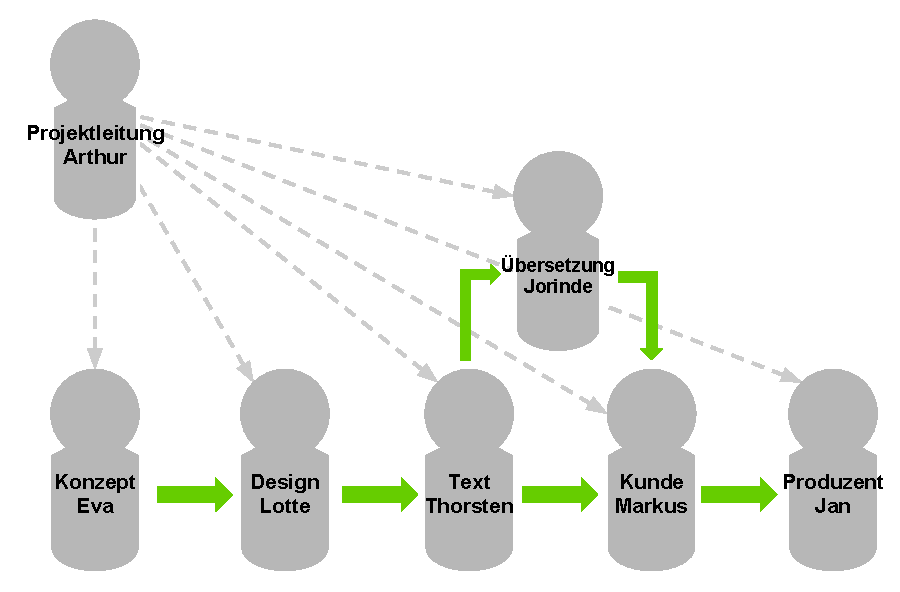
\includegraphics[width=\textwidth]{media/Uebersicht-Personas.pdf}
\caption{Übersicht über die Personas und den idealisierten Workflow}
\label{chart:uebersicht-personas}
\end{center}
\end{figure}

Die Auswahl der Personas orientiert sich an dem vorherrschenden Workflow innerhalb der Projekte. Wie in Kapitel \ref{l:problemanalyse} (S.\pageref{l:problemanalyse}) gezeigt wurde, gibt es in der Praxis keinen linearen Ablauf, sondern es ergeben sich vielzählige Feedback-Schleifen. Vernachlässigt man diese Feedback- und Korrekturschleifen kann man die beteiligten Personen in eine, in Abbildung~\ref{chart:uebersicht-personas} (S.\pageref{chart:uebersicht-personas}) gezeigte, lineare Reihenfolge bringen:
\begin{samepage}\begin{enumerate}\itemsep -5pt
\item Konzepterin \emph{Eva} entwickelt das Produkt, wobei sie die Rahmenbedingungen wie Aufbau, Umfang, Zielgruppe, Ansprache festlegt. 
\item Designerin \emph{Lotte} gestaltet das Produkt, wobei sie bestimmt, wie Texte dargestellt werden (Satz, Länge, Schriftart, Farben, Hervorhebungen)
\item Texter \emph{Torsten} erstellt die Texte für das Produkt in der Ausgangssprache
\item Kunde \emph{Markus} nimmt die Texte ab
\item Übersetzerin \emph{Jorinde} übersetzt die Texte
\item Produzent \emph{Jan} übernimmt die Texte in das Produkt
\end{enumerate}\end{samepage}

Eine wichtige Rolle fehlt in dieser Auflistung: Projektleiter \emph{Arthur} koordiniert den Ablauf des Projektes, hat aber keinen Einfluss den Text. Er darf jedoch als wichtiges Bindeglied zwischen allen Beteiligten  nicht fehlen.

Bei der Formulierung der Personas wurde bewusst darauf verzichtet, persönliche Daten wie Alter und Bildung zu verwenden, da diese keinen Einfluss auf die Konzeption des Systems haben. Die Personas enthalten dementsprechend nur 
\begin{itemize}\itemsep -5pt
\item den wichtigsten Nutzen aus der Sicht der Person als Zitat
\item eine Beschreibung der Aufgabe der Rolle, die diese Persona repräsentiert
\item Angaben zu den Beteiligten, mit denen sich die Person im Verlauf des Projektes \emph{über Texte} austauschen wird
\item die verwendeten Werkzeug zur Erfüllung der Aufgabe und die Erfahrung im Umgang mit Anwendungen im Allgemeinen
\item die wichtigsten Szenarien, die die Persona mit Hilfe des Systems durchführen wird
\item allgemeine Anforderungen an das System
\item und Angaben darüber, wie der Zugriff auf das System erfolgt.
\end{itemize}

\bigskip

Diese Information zusammen mit der Problemanalyse im vorangegangenen Kapitel bilden die Basis für die Konzeption einer Lösung im nächsten Kapitel (\ref{l:konzeption}, S.\pageref{l:konzeption}).

\pagebreak

\subsection{\emph{Eva}, Konzepterin}\label{p:eva}

\begin{multicols}{2}

\begin{center}
\fbox{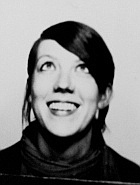
\includegraphics[width=0.5\columnwidth]{media/eva.jpg}}
\end{center}

\citequotes{Ich möchte, dass alle Beteiligten einen guten Überblick über das Produkt haben.}

Eva konzipiert als Informationsarchitektin das Produkt. Dabei legt sie entsprechend der Zielsetzung fest, wie das Produkt aufgebaut ist um die Erwartungen des Nutzers zu erfüllen und ihn das gewünschten Ergebnis im Sinne des Produktes leicht erreichen zu lassen. Hierzu erstellt sie einen Überblick über das Produkt mit Hilfe von Wireframes und macht dabei Vorgaben über die Platzierung von Texten und deren Funktion.

\textbf{Organisation, Abstimmung}

Eva arbeitet auf Seite der Agentur und stimmt sich mit \emph{Markus}~(\ref{p:markus}) sowie \emph{Lotte}~(\ref{p:lotte}) über das Produkt ab. Sie gibt Feedback zu den Texten von \emph{Torsten}~(\ref{p:torsten}) und deren Integration in das Produkt durch \emph{Jan}~(\ref{p:jan}).

\textbf{Werkzeuge und Erfahrung}

Evas wichtigstes Werkzeug ist \trademark{OmniGraffle} von \trademark{Omni Group} mit dem sie die Wireframes des Produktes erstellt. Sie ist versiert im Umgang mit vielfältigen Anwendung und steht neuen Werkzeugen offen gegenüber.

\columnbreak

\textbf{Szenarien}

Eva definiert die einzelnen logischen Bestandteile des Produktes (z.B. Seiten, Abschnitte) und definiert darin, welche einzelnen Textbausteine verwendet werden.

Eva legt Rahmenbedingungen für den Text fest. Zum einen bestimmt sie die Ansprache, d.h. welche Zielgruppe soll mit den Texten angesprochen werden und welches Ziel verfolgen die Nutzer. Zum anderen macht sie Vorgaben über den Aufbau einzelner Klassen von Texten wie z.B. Überschriften, Schaltflächen, Fließtext bei denen sie z.B. die Textlänge, Spaltenbreite oder Zeilenanzahl festlegt. Diese Rahmenbedingungen kann sie zu den jeweiligen Textbausteinen hinterlegen.

Eva kann sich eine Übersicht ausdrucken, die alle Bestandteile des Produktes enthält. So kann sie leicht den Überblick behalten.

\textbf{Anforderungen}

Eva verwendet das System häufig, deswegen müssen Funktionen zur Definition des Produktes, der Texte und der Rahmenbedingungen einfach zu bedienen sein. Sie will nie die Übersicht verlieren und leicht Elemente verändern können, da sich in der Konzeptionsphase häufig Änderungen ergeben. 

\textbf{Zugang}

Eva greift auf das System mit ihrem \trademark{MacBook Pro} zu, sie verfügt über einen zusätzlichen großen Bildschirm und eine schnelle Internetverbindung.

\end{multicols}

\pagebreak

\subsection{\emph{Lotte}, Designerin}\label{p:lotte}

\begin{multicols}{2}

\begin{center}
\fbox{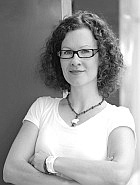
\includegraphics[width=0.5\columnwidth]{media/lotte.jpg}}
\end{center}

\citequotes{Ich möchte, dass meine Vorgaben zur Gestaltung der Texte von allen berücksichtigt werden.}

Lotte gestaltet als Art-Direktorin das Produkt. Sie entwirft dazu das Fein-Layout auf Basis der Wireframes, die von \emph{Eva}~(\ref{p:eva}) erstellt wurden, indem sie für alle Darstellungs-Varianten präzise Entwürfe anfertigt. Hierbei legt sie auch genaue Vorgaben für die Formatierung der Texte im Produkt fest.

\textbf{Organisation, Abstimmung}

Lotte arbeitet auf Seiten der Agentur und stimmt sich mit \emph{Eva}~(\ref{p:eva}) bei der Gestaltung des Produktes ab. Mit \emph{Torsten}~(\ref{p:torsten}) spricht sie über ihre Vorgaben zu Texten und überprüft deren Einhaltung in der Umsetzung durch \emph{Jan}~(\ref{p:jan}).

\textbf{Werkzeuge und Erfahrung}

Lotte arbeitet mit den Produkten der \trademark{Adobe Creative Suite}. Sie ist nur im Umgang mit wenigen anderen Werkzeugen versiert, steht neuen Anwendungen aber offen gegenüber.

\textbf{Zugang}

Lotte greift auf das System mit ihrem \trademark{iMac} zu, sie verfügt über einen großen Bildschirm und eine schnelle Internetverbindung.

\columnbreak

\textbf{Szenarien}

Lotte erstellt einen Styleguide und legt dabei fest, welche Text-Klassen im Produkt verwendet werden. Text-Klassen sind z.B. Überschriften, Untertitel und Fließtext. Dazu macht sie für jede Klasse Angaben zu der verwendeten Schriftart, die Einschränkungen, wie z.B. die maximalen Zeilenanzahl oder Menge der Zeichen pro Zeile.

Lotte erstellt Layouts in Form von Screenshots oder Beispielseiten. Hierbei verwendet Sie für die Texte die noch nicht durch \emph{Eva}~(\ref{p:eva}) festgelegt wurden, Blindtexte. Um ein besseres Gefühl für die Inhalte zu bekommen und die Layouts besser mit dem Kunden abstimmen zu können möchte Lotte gerne jetzt schon einige Texte von \emph{Torsten}~(\ref{p:torsten}) in den Layouts verwenden.

Während der Umsetzung des Produktes ergeben sich Änderungen am Styleguide. Sie möchte, dass \emph{Jan}~(\ref{p:jan}) alle Stellen im Produkt anpasst, die von dieser Änderungen betroffen sind.

\textbf{Anforderungen}

Lotte möchte das Anlegen von Text-Vorgaben unkompliziert und schnell erledigen können. Änderungen müssen jederzeit und ohne großen Aufwand möglich sein. Das System muss leicht verständlich sein, da sie nie viel Zeit damit verbringt. Komplizierte Abläufe würden Sie abschrecken und sie würde statt dessen eine E-Mail schreiben.

Lotte hat sehr hohe Ansprüche an die Gestaltung des Systems.

\end{multicols}

\pagebreak

\subsection{\emph{Torsten}, Texter}\label{p:torsten}

\begin{multicols}{2}

\begin{center}
\fbox{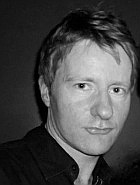
\includegraphics[width=0.5\columnwidth]{media/torsten.jpg}}
\end{center}

\citequotes{Ich möchte den Texteditor an meine Bedürfnisse anpassen können und beim Schreiben in meinem \typoquotes{Flow} nicht unterbrochen werden.}

Torsten erstellt auf Basis der vom Kunden gelieferten Materialien oder bereits bestehender Produkte die Texte für das Produkt. Hierbei muss er Vorgaben aus dem Konzept und dem Design berücksichtigen, sowie Wünschen und möglicherweise verbindliche Richtlinien des Kunden beachten. Hierzu erstellt Torsten für alle Textbausteine des Produktes die Texte in der endgültigen Fassung in seiner Muttersprache.

\textbf{Organisation, Abstimmung}

Torsten ist selbständig. Er stimmt sich mit \emph{Eva}~(\ref{p:eva}) und \emph{Lotte}~(\ref{p:lotte}) bezüglich deren Vorgaben ab. Er berücksichtigt inhaltliche Vorgaben, die er von \emph{Markus}~(\ref{p:markus}) erhält. Er steht  \emph{Jorinde}~(\ref{p:jorinde}) für Rückfragen zur Verfügung.

\textbf{Werkzeuge und Erfahrung}

Torsten arbeitet mit \trademark{iWorks Pages} von \trademark{Apple}, da er die vielen Funktionen von \trademark{Word} als störend empfindet und diese nicht benötigt. Er ist nur im Umgang mit wenigen Programmen vertraut.

\columnbreak

\textbf{Szenarien}

Torsten verfasst die Texten zum Produkt, dazu befüllt der die vom Design vorgegeben Textbaustein. Dabei bekommt kann er die Vorgaben sehen, die für den jeweiligen Text gelten (z.B. maximale Textlänge). 

Torsten benötigt Kontext-Information zum aktuellen Text und kann im System die vom Kunden zur Verfügung gestellten Materialien aufrufen. Auch die Hinweise zur Zielgruppe und Funktion des Textes aus dem Konzept kann er sich ansehen, ohne die aktuelle Ansicht des Systems verlassen zu müssen.

Der Kunde wünscht Änderungen an den Texten. Diese sind im System bei den jeweiligen Textbausteinen hinterlegt, so das Torsten die Texte schnell anpassen kann, ohne sie erst aufwändig suchen zu müssen.

Torsten arbeitet in einem Team mit anderen Textern und führt die Qualitätskontrolle an den Texten seiner Kollegen durch.

\textbf{Anforderungen}

Das Editor zum Erstellen von Texten muss im System an Torsten Bedürfnisse anpassbar sein. Er möchte genaue Kontrolle darüber haben, \emph{wann} andere Projektmitarbeiter seine Texte sehen können. Feedback zu Texten soll zu den jeweiligen Textbausteinen zugeordnet werden können.

\textbf{Zugang}

Torsten arbeitet in seinem eigenen Büro oder von unterwegs, da er an mehreren Projekten gleichzeitig arbeitet. Er greift auf das System mit seinem \trademark{MacBook Pro} zu und je nach Standort kann seine Internetverbindung auch nur mittel schnell sein.

\end{multicols}

\pagebreak

\subsection{\emph{Markus}, Kunde}\label{p:markus}

\begin{multicols}{2}

\begin{center}
\fbox{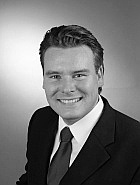
\includegraphics[width=0.5\columnwidth]{media/markus.jpg}}
\end{center}

\citequotes{Ich möchte, dass die Vorgaben aus unserer Marketing"~, Fach"~ und Rechtsabteilung genau berücksichtigt werden. Änderungswünsche und Korrekturen sollen exakt befolgt werden.}

Markus ist der Auftraggeber des Produktes. Er ist der erste Ansprechpartner für die Agentur, steht aber auch stellvertretend für weitere Unternehmensmitarbeiter aus verschiedenen Abteilungen seines Unternehmens. Er liefert Materialien und Vorgaben die als Basis für die zu erstellenden Texte dienen. Er führt auch die finale Abnahme der Texte und des Produktes durch.

\textbf{Organisation, Abstimmung}

Markus stimmt sich über den Zweck des Produktes mit \emph{Eva}~(\ref{p:eva}) ab. \emph{Torsten}~(\ref{p:torsten}) gibt er Feedback und Änderungswünschen zu dessen Texten. Auch die Übersetzungen von \emph{Jorinde}~(\ref{p:jorinde}) kontrolliert und verbessert er. Wurden die Texte in das Produkt übernommen, gibt er Änderungswünsche an den Inhalten und der Darstellung an \emph{Jan}~(\ref{p:jan}) weiter.

\textbf{Werkzeuge und Erfahrung}

Markus arbeitet vor allem mit \trademark{Word}, \trademark{Excel} und \trademark{PowerPoint}, ansonsten hat er keine weiteren Erfahrungen im Umgang mit Werkzeugen.

\columnbreak

\textbf{Szenarien}

Markus nimmt die fertigen Texte ab. Hierzu kann er einzelnen Textbausteine freigeben oder Änderungen anfordern, die er mit Hilfe von Kommentaren beschreibt. 

Um den Projektablauf nicht zu verzögern beantwortet Markus Rückfragen zu Texten von unterwegs.

Materialien können in das System eingestellt und einzelnen Textbausteinen oder ganzen Abschnitten zugeordnet werden.

Markus kann sich alle Texte als \trademark{Word}-Dokument exportieren um Korrekturen darin vorzunehmen. Anschließend importiert er das Dokument. Dabei werden die Änderungen automatisch im System übernommen.

\textbf{Anforderungen}

Das System \citequotes{muss einfach funktionieren}, da er nicht gezwungen werden will, ein neues System zu erlernen. Er erwartet, dass die wichtigen Funktionen auch mobil verfügbar sind. Die Daten im System und der Zugriff darauf müssen sicher sein. Er will festlegen, wer Zugriff erhält, mit der Möglichkeit, dies auch für einzelne Bereiche des Projektes definieren zu können.

\textbf{Zugang}

Markus arbeitet von seinem Büro-PC aus und greift auf das System mit einer schnellen Internetverbindung zu. Er ist viel unterwegs und verwendet dann sein \trademark{iPhone} oder seinen \trademark{iPad}.

\end{multicols}

\pagebreak

\subsection{\emph{Jorinde}, Übersetzerin}\label{p:jorinde}

\begin{multicols}{2}

\begin{center}
\fbox{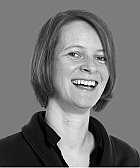
\includegraphics[width=0.5\columnwidth]{media/jorinde.jpg}}
\end{center}

\citequotes{Zum Übersetzen brauche ich eine praktische Darstellung der Original-Texte. Der Zugriff auf Kontext-Informationen muss leicht möglich sein.}

Jorinde übersetzt die Texte des Projektes in ihre Muttersprache. Sie berücksichtigt dabei bestehende Materialien des Kunden, sowie die Vorgaben aus Konzept und Design.

\textbf{Organisation, Abstimmung}

Jorinde arbeitet in einem Übersetzungsbüro als Teil eines Teams von Übersetzern, die das gesamte Projekt übersetzen. Sie stimmt sich mit \emph{Torsten}~(\ref{p:torsten}) bei inhaltlichen Fragen zu Texten ab. Für die Übersetzung spezieller Begriffe stimmt sie sich mit \emph{Markus}~(\ref{p:markus}) ab.

\textbf{Werkzeuge und Erfahrung}

Jorinde verwendet zum Erstellen der Übersetzung \trademark{Word}, da ihr dort Komfortfunktionen wie Rechtschreibkorrektur und Synonyme zur Verfügung stehen.  Jorinde hat wenig Erfahrung mit anderen Werkzeugen und braucht im allgemeinen länger, um sich an neue Systeme zu gewöhnen.

\textbf{Zugang}

Jorinde greift auf das System nur von ihrem Firmen-PC aus zu und verfügt über eine schnelle Internetverbindung.

\columnbreak

\textbf{Szenarien}

Jorinde übersetzt die Texte des Projekts, dazu werden die Originaltexte direkt in der Übersetzungsansicht dargestellt. Die Zusatzinformationen zu den Textbausteinen stehen ihr, wie bei \emph{Torsten}~(\ref{p:torsten}), in der Ansicht zur Verfügung.

Jorinde ist sich bei der Übersetzung eines bestimmten Begriffes unsicher. Sie verwendet das zur Verfügung gestellt Ausgangs-Material des Kunden um die Übersetzung nachzuschlagen, die in Publikationen des Kunden üblicherweise verwendet wird. Für zukünftige Verwendung hinterlegt sie dies im Glossar des Projektes.

Das Projekt enthält an mehreren Stellen die gleichen Formulierungen. Jorinde erhält an diesen Stellen die Übersetzung vorgeschlagen, die sie bereits angelegt hat. Sie kann diese direkt übernehmen oder eine Variante anlegen.

Jorinde sucht für einen Begriff ein Synonym. Sie kann sich direkt in der Ansicht zu dem Begriff Synonyme aus einem globalen Wörterbuch anzeigen lassen. Zusätzlich kann sie sich für das Wort in der Orginalsprache die Übersetzungen anzeigen lassen, die bereits im Projekt verwendet wurden.

Jorinde führt die Qualitätskontrolle an übersetzten Texten ihrer Kollegen durch.

\textbf{Anforderungen}

Jorinde benötigt zum Übersetzen im System die Hilfsmittel, die ihr auch in \trademark{Word} zur Verfügung stehen: Rechtschreibkorrektur, Synonyme sowie die nahtlose Integration von Wörterbüchern in mehreren Sprachen.

\end{multicols}

\pagebreak

\subsection{\emph{Jan}, Produzent}\label{p:jan}

\begin{multicols}{2}

\begin{center}
\fbox{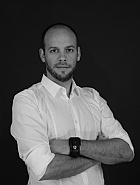
\includegraphics[width=0.5\columnwidth]{media/jan.jpg}}
\end{center}

\citequotes{Ich muss exakt wissen, welche Texte an welche Stelle im Produkt gehören. Bei Änderungen am Text möchte ich nicht jedes mal die Texte per Copy\&Paste übertragen müssen.}

Jan ist für die Erstellung des Produktes verwantwortlich. Er hat aber auch während der Entwurfsphase Einfluss auf die Rahmenbedingungen für Texte, vor allem wenn es um technische Parameter geht (z.B. maximale Zeilenlänge).

\textbf{Organisation, Abstimmung}

Jan arbeitet auf Seiten der Agentur und stimmt sich mit \emph{Eva}~(\ref{p:eva}) über den Aufbau und mit \emph{Lotte}~(\ref{p:lotte}) über die Gestaltung des Produktes ab. Von \emph{Markus}~(\ref{p:markus}) bekommt er letzte Änderungen am Text mitgeteilt, die erst bei der Darstellung im fertigen Produkt auffallen.

\textbf{Anforderungen}

Für Jan ist es sehr wichtig, dass er die Texte am besten automatisiert in seine Werkzeuge übernehmen kann, so dass Texte, die bereits in das Produkt integriert wurden bei Änderungen automatisch aktualisiert werden können. Für Software-Produkte erwartet er, dass der Zugriff auf die Texte mit einer API möglich ist.

\columnbreak

\textbf{Szenarien}

Jan hat eine Broschüre in \trademark{Adobe InDesign} erstellt. Er verknüpft die Texten aus dem System mit den Texten im Dokument. Nachdem sich bereits verwendete Texte geändert haben, öffnet Jan das Dokument erneut und kann mit Hilfe eines Dialoges die geänderten Stellen anspringen. Er muss diese nur noch auf gestalterische Probleme hin kontrollieren.

Jan hat eine \trademark{Android}-App entwickelt und verwendet die Identifier der vom Konzept vorgegebenen Texte. Beim kompilieren der App lädt das build-Script die aktuellen Texte für die App über die Schnittstelle des Systems und erzeugt automatisch die Sprachdateien.

Jan entdeckt ein Problem mit der Textlänge einer Überschrift. Er meldet dieses Problem im System. \emph{Lottes}~(\ref{p:lotte}) Änderungen betreffen allen Überschriften. Jan kann sich im System alle betroffenen Stellen im Produkt anzeigen lassen.

\textbf{Werkzeuge und Erfahrung}

Jan arbeitet je nach Produkt mit DTP-Produkten oder IDEs (für diese Persona ist es unerheblich, ob ein Medium oder Software entsteht), er ist versiert im Umgang mit vielen Werkzeugen und kann sich sehr schnell in neuen Anwendungen eingewöhnen.

\textbf{Zugang}

Jan greift von seinem Laptop aus auf das System zu. Er verfügt über eine schnelle Internetverbindung.

\end{multicols}

\pagebreak

\subsection{\emph{Arthur}, Projektleiter}\label{p:arthur}

\begin{multicols}{2}

\begin{center}
\fbox{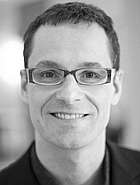
\includegraphics[width=0.5\columnwidth]{media/arthur.jpg}}
\end{center}

\citequotes{Ich möchte steuern, wer welche Aufgabe im Projekt übernimmt und über Problemen informiert sein. Ich möchte jederzeit einsehen können, welcher Anteil der Texte bereits fertig ist.}

Arthur koordiniert als Projektleiter mit allen Beteiligten den Ablauf des Projektes, hat jedoch keinen Einfluss auf die eigentlichen Texte.

\textbf{Organisation, Abstimmung}

Arthur arbeitet auf Seiten der Agentur und stimmt sich über organisatorische Fragen mit allen Beteiligten ab.

\textbf{Werkzeuge und Erfahrung}

Arthur arbeitet vor allem mit \trademark{Word}, \trademark{Excel} und \trademark{PowerPoint}, findet sich aber leicht in anderen Anwendungen zurecht.

\textbf{Anforderungen}

Für Arthur muss das System vor allem immer verfügbar sein, Unterbrechungen im Projektverlauf durch einen Systemausfall sind nicht akzeptabel. Auch ein Datenverlust muss ausgeschlossen sein. Es muss möglich sein alle Daten des Projektes zu exportieren.

\columnbreak

\textbf{Zugang}

Arthur greift von seinem Laptop auf das System zu und verfügt über eine schnelle Internetverbindung.

\textbf{Szenarien}

Arthur legt ein neues Projekt an und fügt Mitarbeiter mit Hilfe ihrer E-Mail-Adressen hinzu. Er kann Mitarbeitern Rollen zuweisen, damit klar ist, welche Aufgabe sie haben. 

Die Rechtsabteilung des Kunden muss die AGB, das Impressum und die Datenschutzbedingungen einer Website abnehmen. Arthur konfiguriert den Workflow im System so, dass diese Texte von allen Mitarbeitern dieser Abteilung freigegeben werden müssen.

Arthur beauftragt ein Lektorat mit der Kontrolle aller Texte. Er konfiguriert den Workflow so, dass Texte erst durch den Kunden einsehbar sind, wenn die Mitarbeiter des Lektorats alle geprüft haben.

Anhand der Aufzeichnungen seit Projektbeginn kann das System für Arthur einen voraussichtlichen Abschlusstermin berechnen. Es ist ersichtlich, dass der Texter für die Erstellung seiner Texte zu lange braucht. Arthur zieht einen Texter aus einem anderen Projekt ab und weist ihn diesem Projekt zu. Das System berechnet mit der zusätzlichen mittleren Arbeitsleistung des neuen Texters ein neues Enddatum, das jetzt Arthurs Vorstellung entspricht.

\end{multicols}

\pagebreak


\pagebreak

\section{Konzeption einer an den spezifischen Workflow angepassten Anwendung}\label{l:konzeption}

Im Abschnitt~\ref{l:problemanalyse}~(S.\pageref{l:problemanalyse}~ff.) wurde analysiert, welche Probleme in Zusammenhang mit der Produktion von Informations- und Kommunikationsmedien bezüglich den verwendeten Texten entstehen, wenn Textverarbeitungs- und Tabellenkalkulationsprogramme wie \trademark{Microsoft} \emph{Word} und \trademark{Excel} verwendet werden. Aus dieser Analyse wurde die Schlussfolgerung gezogen, dass eine browserbasierte Web-Anwendung am besten geeignet ist, den Workflow und alle Beteiligten zu integrieren. Dies wird in Abschnitt~\ref{l:loesungsart} ausführlich begründet. Im vorangegangenen Abschnitt~\ref{l:personas}~(S.\pageref{l:personas}~ff.) wurden Personas vorgestellt, die repräsentativ für die Benutzer der Anwendung stehen. Deren Anforderungen an das System und die Analyse des spezifischen Workflows in Abschnitt~\ref{l:workflow} bilden die Grundlage für Erstellung einer Liste von Anforderungen an die Lösung in Abschnitt~\ref{l:anforderungen}. Auf dieser Basis kann in Abschnitt~\ref{l:entwurf} die Anwendung entworfen werden.

\bigskip

Eine Implementierung der Anwendung in Form eines Prototypen erfolgt im nächsten Abschnitt~\ref{l:implementierung}~(S.\pageref{l:implementierung}~ff.).

\subsection{Art der Anwendung}\label{l:loesungsart}

Das System wird als \emph{browserbasierte Web-Anwendung mit vollständiger Schnittstellen-Abdeckung} konzipiert. 

\begin{figure}[htb]
\begin{center}
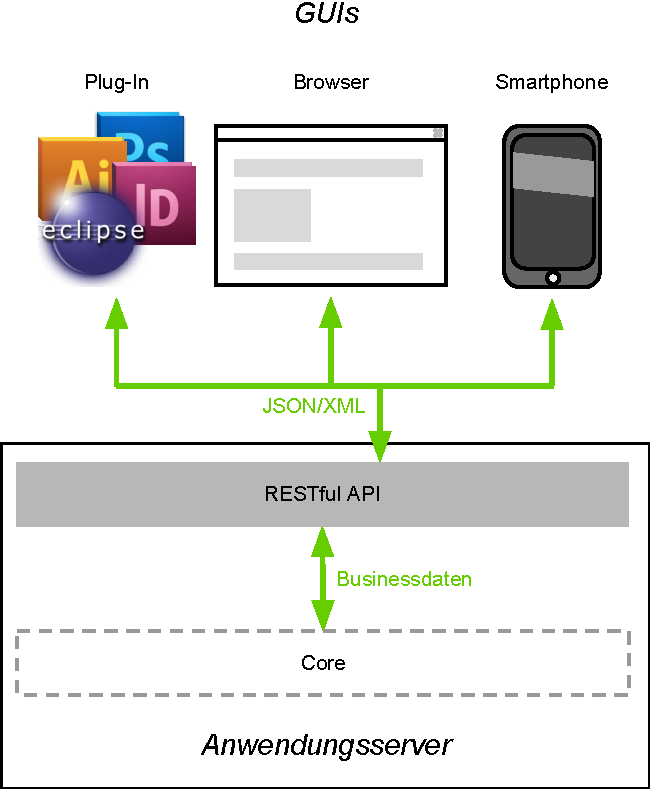
\includegraphics[width=0.65\textwidth]{media/ArtdesSystems.pdf}
\caption{Aufbau des System in stark vereinfachter Darstellung}
\label{chart:aufbaudessystems}
\end{center}
\end{figure}

\subsubsection{Browserbasierte Web-Anwendung} 

Diese Klasse von Anwendung verwendet einen Webbrowser als Laufzeitumgebung. Dabei stellt der Browser das GUI der Anwendung mit Hilfe von HTML, CSS und JavaScript dar, die Businesslogik und die Datenhaltung wird auf einem Server ausgeführt, mit der die GUI mithilfe einer Schnittstelle kommuniziert. Abbildung~\ref{chart:aufbaudessystems}~(S.\pageref{chart:aufbaudessystems}) zeigt den Aufbau des Systems in stark vereinfachter Darstellung. War es in den letzten Jahren noch üblich, dass Fragmente des GUIs mit serverseitigen Template-Sprachen erzeugt wurden (vgl.~\cite[S.48]{dunkel2008systemarchitekturen}) hat die zunehmende Verbreitung von mobilen Clients ein Umdenken zur Folge. Zum einen stellen Desktop-Clients, mobile Browser-Clients und native Apps zwar die gleichen Daten eines Systems dar, verwenden dafür aber nicht zwangsläufig die gleiche GUI-Technologie. Zum anderen werden Clients immer leistungsstärker, selbst Einsteiger-SmartPhones haben inzwischen CPUs mit mindestens dreistelligem Megahertz-Wert. Diese Entwicklung führt gerade bei Web-Anwendungen, auch Rich Internet Applications (RIAs) genannt, zu der Idee, Architekturen zu entwickeln, bei denen serverseitig keine GUI-Komponenten mehr erzeugt werden (vgl.~\cite{maccaw2011javascript} und \cite{coates2012phptemplating}). Clients kommunizieren über Schnittstellen mit dem Server und tauschen nur noch reine Daten aus. Dies hat mehrere Vorteile. Zum einen muss serverseitig kein Modell der clientseitigen Darstellung verwaltet werden, zum anderen verkleinert sich die Menge der transferierten Daten zwischen Client und Server erheblich. Dies hat besonders bei Benutzern mit langsamen oder schlechten Datenverbindungen im Mobilfunk-Netz große Vorteile. Für Webanwendungen bedeutet dass diese das zur Darstellung benötigte HTML mit Hilfe von JavaScript selber direkt im Client erzeugen. Beim ersten Besuch einer Internetseite müssen lediglich einmal die JavaScript-Dateien und benötigte statische Ressourcen wie CSS-Dateien, Bilder und ein statischer HTML-Grundaufbau geladen werden. Anschließend werden nur noch die für die jeweilige Aktion benötigten Daten mit Hilfe von JavaScript zwischen der Anwendung und dem Server ausgetauscht. Mobile Endgeräte, die über eigene GUI-Toolkits verfügen, oder Software von Drittanbietern können dann die selben Schnittstellen verwenden, ohne dass serverseitige Anpassungen vorgenommen werden müssen. 

Web-Anwendung haben den Vorteil, dass sie ohne Installation auf dem Rechner des Benutzers lauffähig sind. Sie können als unmittelbar verwendet werden. Kompaitibilätsprobleme mit alten Browser-Versionen (z.B. dem \trademark{Internet Explorer 6}) können inzwischen mit Hilfe des \trademark{ChromeFrame}\footnote{\url{https://developers.google.com/chrome/chrome-frame/}} komfortable umgangen werden. Der Umfang an frei verfügbaren Bibliotheken zur Erstellung attraktiver und angenehm benutzbarer Anwendungen auf Basis von HTML ist riesig. Web-Anwendungen können mit wenig Aufwand auch auf mobilen Endgeräten eingesetzt werden, da Technologien zur platformabhängigen Anpassung der Darstellung (z.B. CSS-Mediaqueries) existierten. Insgesamt sind Webbrowser der aktuellen Generation mächtige Werkzeuge zur Erstellung von CRUD-Anwendungen. \cite{ms-key-software-development-trends} Die allgemeinen Vorteile einer browserbasierten Software, auch als \emph{Software as as Service} (SaaS) oder \emph{Application Service Provider} (ASP) Modell bekannt, liegen auf der Hand und werden an dieser Stelle nicht detailliert ausgeführt. Um nur einen zu nennen: die Möglichkeit, die Software jederzeit und für alle Mitarbeiter gleichzeitg ohne deren Zutun aktualisieren zu können, eliminiert vielfältige Probleme, die sonst in Umgebungen entstehen, in denen unterschiedliche Programmversionen existieren.

\subsubsection{Schnittstellen} 

Die Verwenden einer einheitlichen Schnittstelle durch alle Clients ermöglicht ein konsistentes Verhalten der Anwendungen über alle Zugangswege hinweg und ist besonders in Fall dieser Anwendung von Bedeutung, da die Benutzer des Systems wünschen, dass sich die Texte direkt innerhalb ihrer bevorzugten Werkzeuge abrufen und einbinden lassen. Dies ist nur mit Hilfe von Plugin-Ins möglich, die in der jeweiligen Umgebung der Software entwickelt werden müssen. Aus diesem Grund ist es ungvermeidlich, dass für alle Funktionen des Systems eine öffentliche Schnittstelle existiert.

Als Protokoll zur Kommunikation zwischen Clients und Server hat sich REST bewährt. Die Struktur des Protokolls ist direkt mit dem HTTP-Protokoll vebunden, so ist die Verarbeitung von REST-Anfragen serverseitig leicht mit Web-Frameworks zu implementieren, da diese von sich aus bereits für diese Art von Anfragen ausgelegt sind. Clientseitig wird lediglich ein HTTP-Client benötigt sowie Module zum Parsen von JSON- oder XML-Datenstrukturen -- Voraussetzungen, die von Browsern und SmartPhones erfüllt werden. JSON hat im Vergleich zu SOAP den Vorteil, dass es nicht versucht die Architektur der zugrundeliegenden Software nach außen abzubilden, so muss sich der Client nicht an bestimmte Reihenfolgen im Aufruf von Methoden halten. In der REST-Welt sind alle Operationen atomar und können ohne Vorbedingung gestellt werden. In der Praxis ist dies nicht immer umsetzbar, REST fordert serverseitig Zustandslosigkeit, die aber bei Systemen in denen Daten gespeichert und verändert werden nicht realisierbar ist. Aufgrund seines flexibleren Aufbaus, der Möglichkeit ausgewählte Anfragen leicht mit HTTP-Caches zu beschleunigen und der freien Wahl der Nachrichtenformats ist REST aus Sicht des Autors die besser Wahl zur Implementierung der Schnittstellenkommunikation.

\subsubsection{Zugang}

Diese Konzept macht es möglich, jedem Mitarbeiter den passenden Zugang zu ermöglichen, im Einzelnen sind das:

\paragraph{Browserbasierter Zugang vom Desktop} Den Webbrowser werden alle Mitarbeiter verwenden, da in diesem GUI alle Funktionen der Anwendung implementiert sind.

\paragraph{Browserbasierter Zugang von SmartPhones} Auf gängigen SmartPhones sind Browser vorhanden, die in der Lage sind, die selben Inhalten anzuzeigen, wie ihr Desktop-Equivalent. Aufgrund der deutlich kleineren Bildschirmgröße und dem fehlen einer Maus ist es aber sinnvoll, dem Rechnung zu tragen und eine angepasste Version der Anwendung für diese Geräte bereit zustellen. 

\paragraph{Zugang direkt über die Schnittstellen} Vor allem im Bereich der Software-Entwicklung wird der direkte Zugriff der Entwickler auf die Schnittstellen der Anwendung eine wichtige Rolle spielen. So können diese die Integration des Systems in ihren Entwicklungsprozess optimal an die jeweiligen Bedürfnisse anpassen.

\paragraph{Exporte} Die Möglichlichkeit, die Texte des Projektes in verschiedene Formate zu exportieren ist eine wichtige Funktion. Sie ermöglicht zum einen die Übernahme in System und Programme, deren Anbindung nicht möglich oder gewünscht ist und schafft zum anderen die Möglichkeit, ähnlich wie Schnittstellen, die verarbeiteten Daten auf eine Art und Weise zu verwenden, die nicht vorhergesehen wurde oder nicht im Sinne der Anwendung liegt.

\paragraph{Zugang über Plug-Ins} Besonders für Mitarbeiter in der Produktion kann es wichtig sein, auf ihre angestammten Werkzeuge nicht verzichten zu müssen. Plug-Ins, also Erweiterungen für diese Werkzeuge, integrieren dann Teile der Funktionen der Anwendung in diese Werkzeuge. Beispielsweise könnte es ein Plug-In für \trademark{Adobe InDesign} ermöglichen, auf die Texte aus dem System zuzugreifen und diese direkt in Text-Rahmen im \trademark{InDesign}-Dokument zu übernehmen, so dass Copy\&Paste der Texte aus der Webanwendung oder einem exportierten Dokument entfallen kann.

\paragraph{Benachrichtigungen} Benachrichtigungen sind eine Form des Zugangs, die es Benutzern des Systems ermöglicht, über bestimmte Ereignisse informiert zu werden. Benachrichtigungen können in Form von E-Mails, SMS, über soziale Netzwerke wie Twitter, über Chat-Dienste wie Skype, IRC statt finden. Hierbei werden Information zu einem Ereignis übertragen z.B. der Status-Änderungen eines Textes. Denkbar sind auch auch Push-Exporte der Texte aufgrund eines bestimmten Ereignisses, z.B. der FTP-Export der Texte als CSV-Datei, sobald das Projekt abgschlossen ist oder Änderungen freigegeben wurden.

\paragraph{Software von Drittanbietern} Dadurch, dass alle Funktionen der Anwendung über eine Api exponiert werden, sind auch fremde Softwarehersteller in der Lage, Teile der Funktionen oder die gesamte Anwendung in einer eigenen GUI zu implementieren. So können Bedürfnisse von Anwendergruppen mit besonderen Anforderungen abgedeckt werden, die bei der Konzipierung der Anwendung nicht berücksichtigt wurden.

\subsubsection{Überblick}

Abbildung~\ref{chart:gesamtessystem}~(S.\pageref{chart:gesamtessystem}) liefert einen Überblick über den Aufbau des gesamten Systems:

\begin{figure}[htb]
\begin{center}
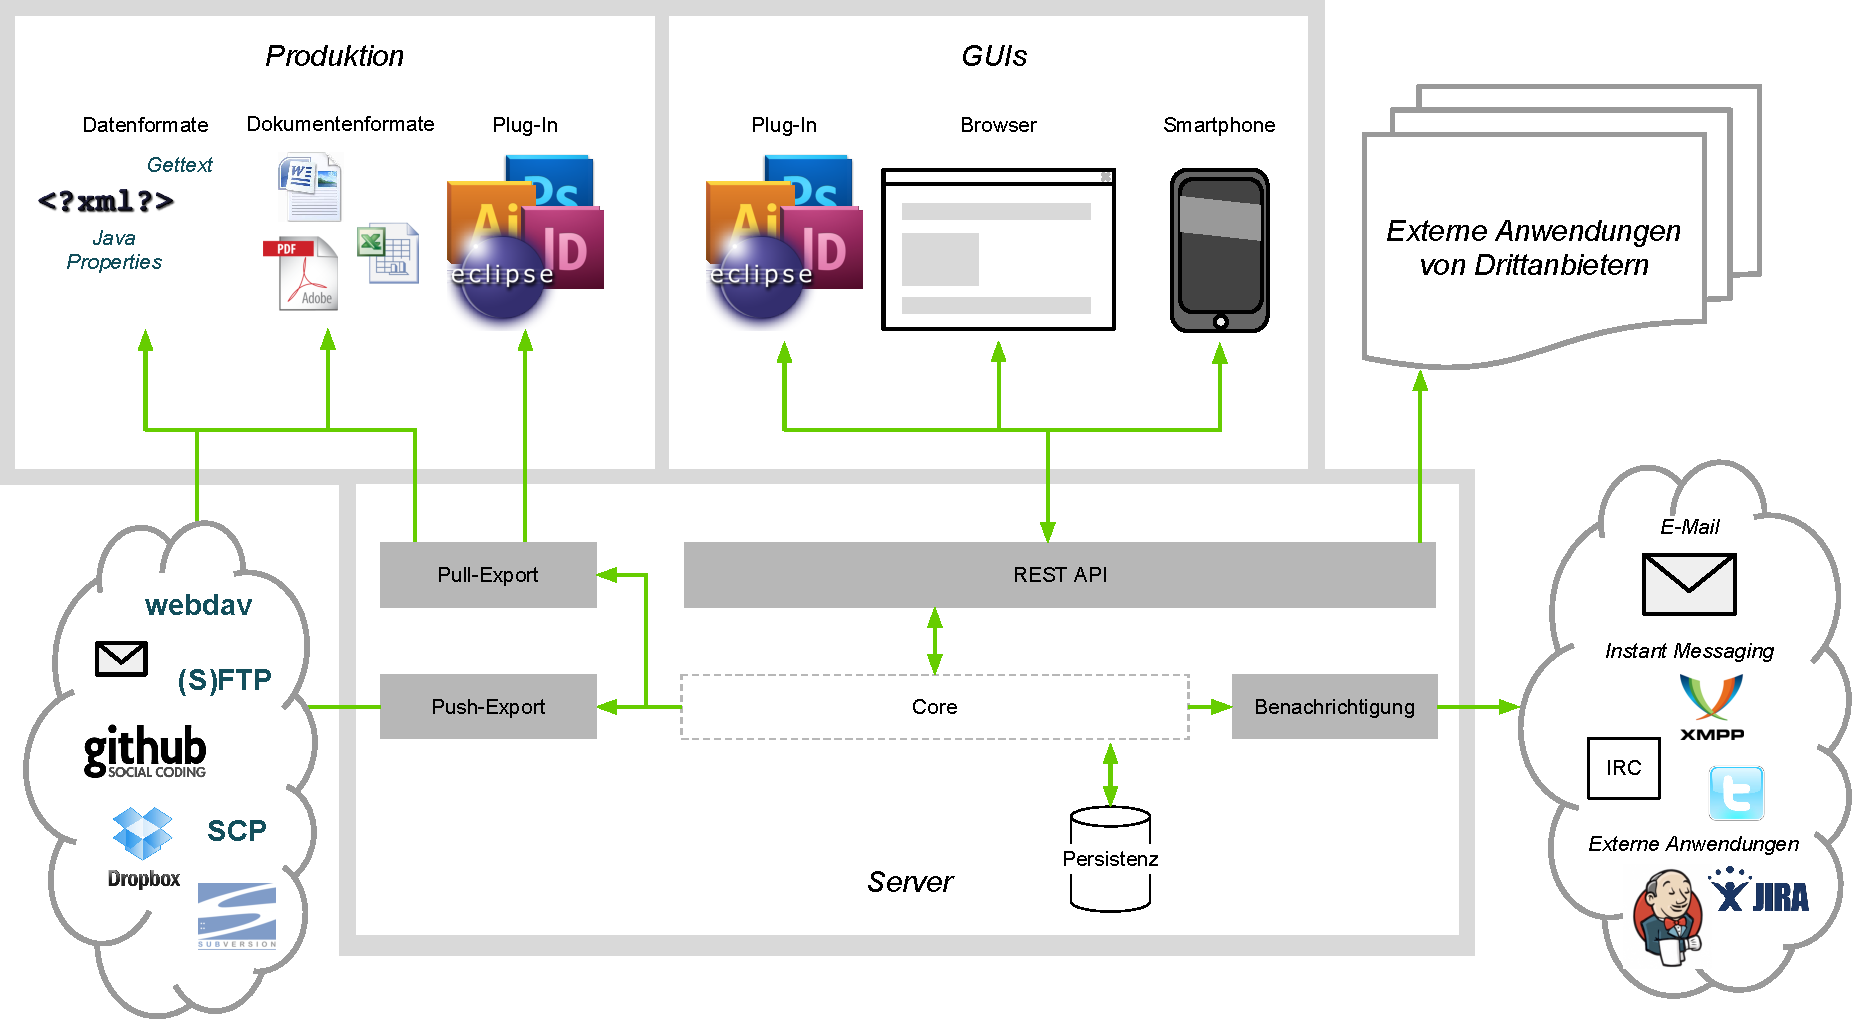
\includegraphics[width=\textwidth]{media/GesamtesSystem.pdf}
\caption{Aufbau des gesamten Systems im Überblick}
\label{chart:gesamtessystem}
\end{center}
\end{figure}

Die Zentrale Komponente der Anwendung bildet der Server. Für die Benutzer erfolgt der Zugriff mit Hilfe einer GUI, die mit der REST-API des Servers kommuniziert. Eine browserbasierte GUI auf Basis von HTML5 und JavaScript bildet den Hauptzugang zum System, der auch auf SmartPhones verwendet werden kann. Zusätzlich gibt es spezielle Plugins für Adobe-Produkte und weitere wichtige Produktionsumgebungen. Auch native GUIs für Smartphones verwenden die gleiche API. Die Schnittstellen können auch von Drittanbietern dazu verwendet werden, eigenen Clients für das System zu entwickeln. In die Endprodukte gelangen die Texten über den Export, exportiert wird dabei in viele Formate, neben Datenformaten wie z.B. XML werden auch Dokumentenformate wie z.B. Word exportiert. Der Export kann durch den Anwender erzeugt werden (\emph{Pull-Export}), aber auch automatisch, z.B. nach festgelegten Zeitplänen oder Ereignissen erfolgen. Dieser \emph{Push-Export} erfolgt auf je nach Projekt festlegbaren Orte, wie z.B. FTP-Server oder Versionsverwaltungssysteme. Die Benachrichtigungen über Aufgaben und Änderungen an Texten kann via E-Mail, aber auch mittels Instant-Messaging-Systeme oder durch den Aufruf fremde API-Endpunkte erfolgen.

\subsection{Der spezifische Workflow}\label{l:workflow}

Beobachtet man verschiedene Projekte, in denen Informations- und Kommunikationsmedien erstellt werden, lässt sich feststellen, dass Texte immer wieder auf die gleiche Art beeinflusst werden. Für eine vollständige Beschreibung des Workflows ist es zunächst sinnvoll, zu ermitteln, \emph{wie} Texte beeinflusst werden. 

% MARK

\begin{figure}[htb]
\begin{center}

\includegraphics[width=\textwidth]{media/chart-3.pdf}
\end{center}
\caption{Operationen bei der Erstellung von Texten}
\label{chart:3}
\end{figure}

Betrachtet man die Arbeiten in Zusammenhang mit Text lassen sich diese in sechs eigenständige Operationen unterteilen:

\begin{enumerate}
\item{Durch \textbf{Definieren eines Textbausteines} wird festgelegt, wie der benötigte Text beschaffen sein muss. Die Aussage \typoquotes{Wir brauchen an dieser Stelle eine Überschrift} ist ein Beispiel für diese Operation. Sie legt fest, wie der Textbausteine gestaltet werden muss, um die ihm zugedachte Aufgabe zu erfüllen. Neben der Angabe zur Platzierung auf dem Medium durch \typoquotes{an dieser Stelle} wird implizit durch \typoquotes{eine Überschrift} eine Angabe zur inhaltlichen und visuellen Gestaltung getroffen; Überschriften sollen kurz und knapp sein und ihre visuelle Gestaltung wird durch den Styleguide des Projektes festgelegt.}
\item{Das \textbf{Schreiben eines Textes} befüllt einen Textbaustein mit einem Text in einer Sprache. Bei diesem Vorgang wird der Text entsprechend der Vorgabe aus der Beschreibung als Original erstellt oder aus Quellen außerhalb des Projektes kopiert und eingefügt. }
\item{In der \textbf{Korrektur} wird der Text inhaltlich und grammatikalisch überprüft und entsprechend angepasst. Der Korrektor muss dabei für eine grammatikalische Überprüfung des Textes kein Fachwissen bezogen auf das Projekt haben. Ist diese Fachwissen vorhanden, kann eine inhaltliche Korrektur vorgenommen werden.}
\item{In der \textbf{Qualitätskontrolle} wird der Text dahingehend überprüft, ob er den Anforderungen gemäß der Beschreibung und inhaltlichen Vorgaben, auch hinsichtlich des gesamten Projektes entspricht. }
\item{Durch die \textbf{Freigabe} wird der Text abgenommen und kann nun in das Endprodukt übernommen werden.}
\item{Durch die \textbf{Veröffentlichung} wird der Text in das Endprodukt eingebracht.}
\end{enumerate}

\begin{figure}[htb]
\begin{center}
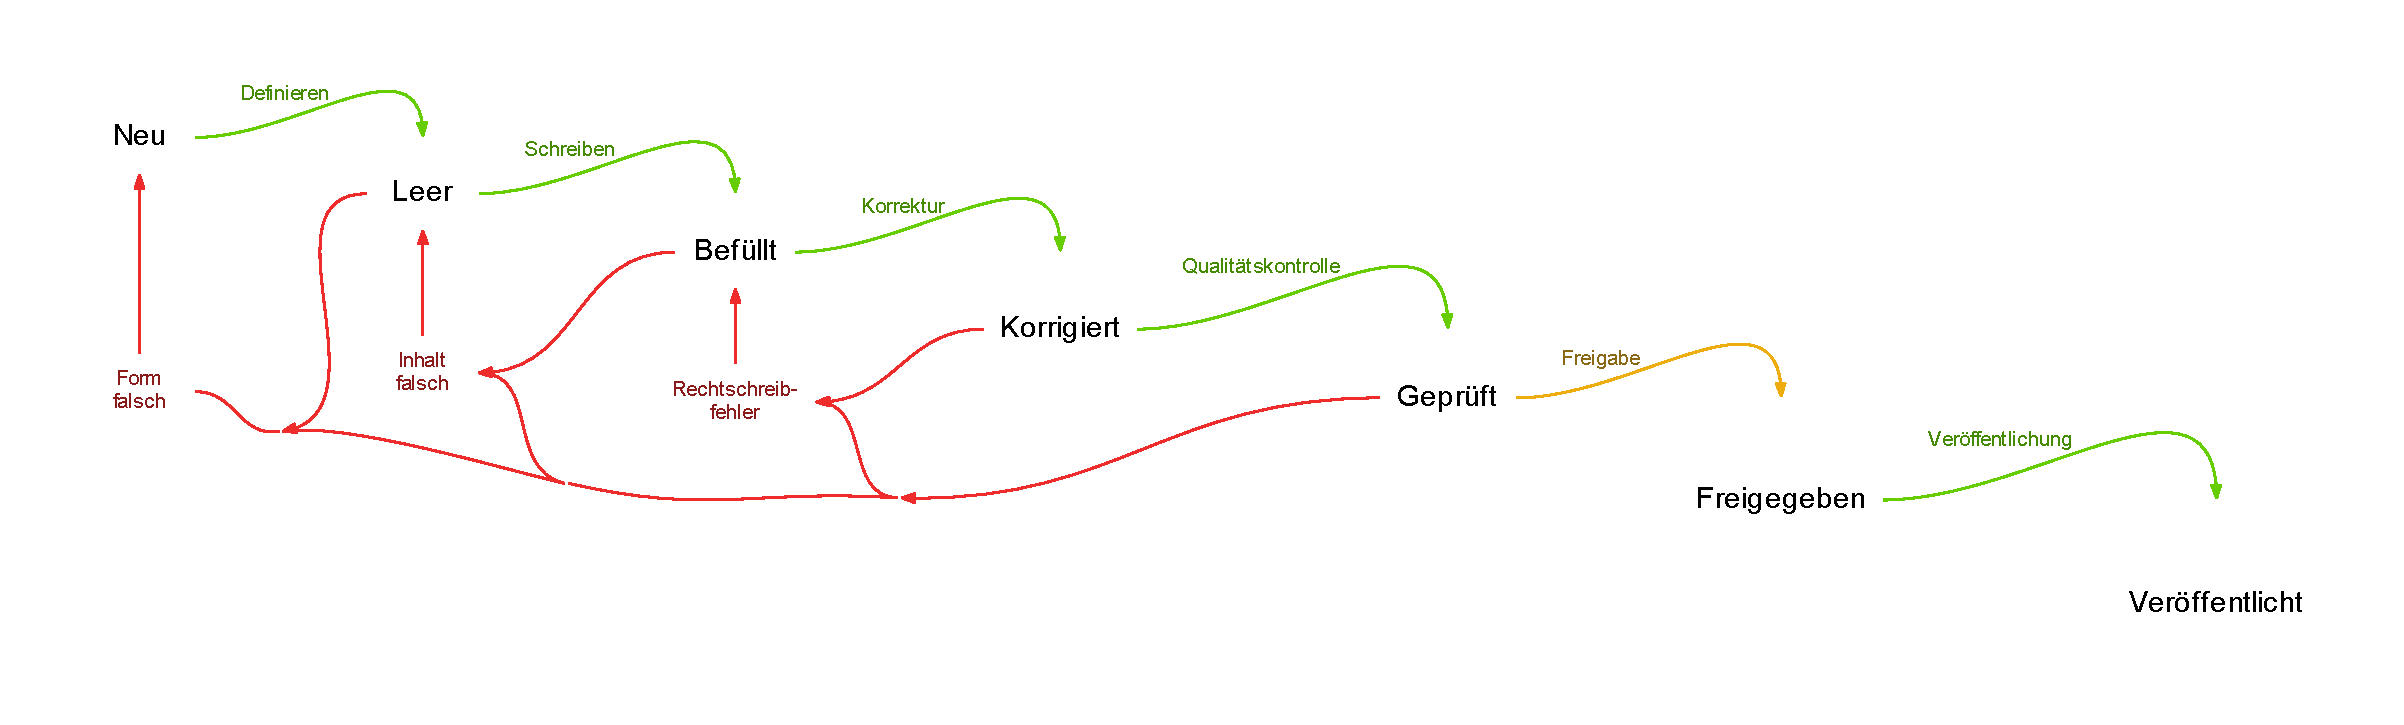
\includegraphics[width=\textwidth]{media/chart-4.pdf}
\end{center}
\caption{Operationen bei der Erstellung von Texten mit Qualitätskontrolle}
\label{chart:4}
\end{figure}

Diese Operationen werden auch 1:1 auf die übersetzte Version eines Textes angewendet.

\begin{figure}[htb]
\begin{center}
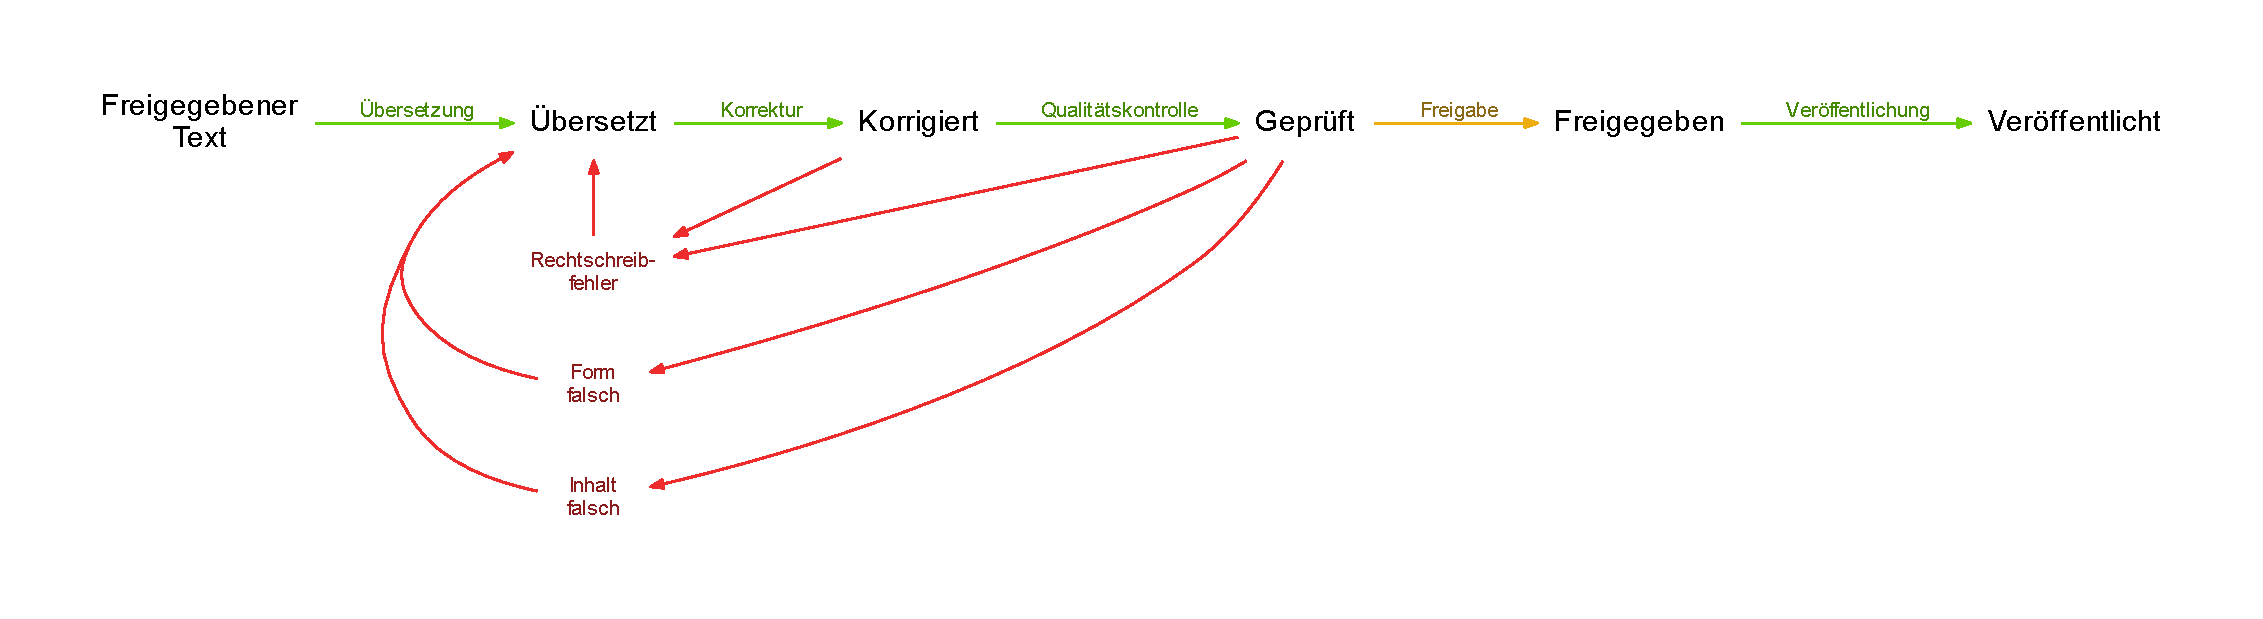
\includegraphics[width=\textwidth]{media/chart-5.pdf}
\end{center}
\caption{Operationen bei der Übersetzung von Texten mit Qualitätskontrolle}
\label{chart:5}
\end{figure}

In Abschnitt~\ref{l:besondererolle} ab Seite~\pageref{l:besondererolle} wurde beschrieben, wie umfangreich die Anzahl der Personen ist, die Einfluss auf die Texte eines Produktes haben. Die Rollenverteilung ist dabei von Projekt zu Projekt unterschiedlich. Allen gemeinsam ist aber, dass die beteiligten Personen  Einfluss auf drei grundlegenden Eigenschaften von Text haben: den Inhalt des Textes, die Attribute wie z.B. \typoquotes{maximale Textlänge} oder \typoquotes{Position im Medium} und den Status wie z.B. \typoquotes{neu} und \typoquotes{freigegeben}. Anhand dieses Kriteriums lassen sich Mitarbeiter in drei Gruppen unterteilen:

% MARK

\paragraph{Personen, die Einfluss auf den Inhalt haben}

\paragraph{Personen, die Einfluss auf den Attribute haben}

\paragraph{Personen, die Einfluss auf den Status haben}




\begin{enumerate}
\item{Der \textbf{Informationsarchitekt} (oder Konzepter) legt die Struktur eines Produktes fest und damit auch die Art und Menge des benötigten Textes,}
\item{der \textbf{Texter} verfasst die Texte,}
\item{der \textbf{Übersetzer} überträgt die Texte in weitere Sprachen,}
\item{der \textbf{Qualitätsmanager} überwacht die Ergebnisse der Prozesse,}
\item{der \textbf{Produktbesitzer} (oder Kunde) ist für die fachlichen und rechtliche Aspekte, sowie das Festlegen der zeitlichen Rahmenbedingungen verantwortlich,}
\item{der \textbf{Produzent} ist für die Erstellung des eigentlichen Produktes verantwortlich.}
\end{enumerate}

Alle Rollen haben im Verlauf eines Projekts, zu unterschiedlichen Zeiten und mit unterschiedlichem Gewicht, Einfluss auf die Gestaltung der Texte. Es existieren auch Abhängigkeiten zwischen den Rollen, so kann ein Übersetzer erst arbeiten, wenn der Text vorliegt und vom Produktbesitzer abgenommen wurde; wird aber zu einem späteren Zeitpunkt der Text geändert, muss auch wieder der Übersetzer neu beginnen.


\subsection{Anforderungen}\label{l:anforderungen}

Wie in der Schlussfolgerung in Abschnitt~\ref{l:schlussfolgerung} bereits erwähnt ergeben sich aus den genannten Problemen im vorangegangenen Kapitel die folgenden Anforderungen an eine Lösung.

\paragraph{Gleichzeitiges Bearbeiten von Texten} Es soll möglich sein, dass alle  Mitarbeiter gleichzeitig an den Texten eines Produktes arbeiten.



\subsection{Eigenschaften von Texten}
\label{l:textattribute}

\paragraph{Typ} Überschrift, Untertitel, Bild-Beschreibung, Fließtext.

\subsection{Beschreibung der notwendigen Funktionalität}

Unterteilung in Muss- und Kann-Kriterien

\subsection{Nachteile/Risiken des Konzepts}

\subsection{Funktionale Anforderungen}

\label{l:anforderungen}

\TODO

Aufteilen der Texte in einzelne Bausteine um diese eindeutig identifizieren zu können. Dies verhindert Copy\&Paste-Fehler (vgl. S.~\pageref{p:serielles-konzept}).

\label{l:hierarchien} Hierarchien sind aber in allen Produkten vorhanden und ein natürlicher Weg, Informationen zu gliedern. 


\subsection{Entwurf}\label{l:entwurf}

Diese vier Leitlinien repräsentieren die Grundgedanken bei der Entwicklung von der Anwendung:

\begin{itemize}
\item{Das wichtigste zuerst: Die aktuelle Aufgabe soll immer im Fokus der Darstellung liegen.}
\item{Schnell zum Ziel: Alle Aufgaben müssen leicht und umkompliziert durchführbar sein.}
\item{Nicht nerven: Ständige Benachrichtigungen lenken ab und müssen deswegen so gestaltet sein, dass diese sich nach den Präferenzen des Nutzers richten.}
\item{Hilfe nur einen Klick entfernt: Das Hilfesystem muss kontextsensitiv verfügbar sein und ist eine Kernfunktion der Anwendung}
\end{itemize}

\subsubsection{Überblick}

Diese Abbildung liefert einen Überblick über den Aufbau des Systems:

\begin{figure}[htb]
\begin{center}
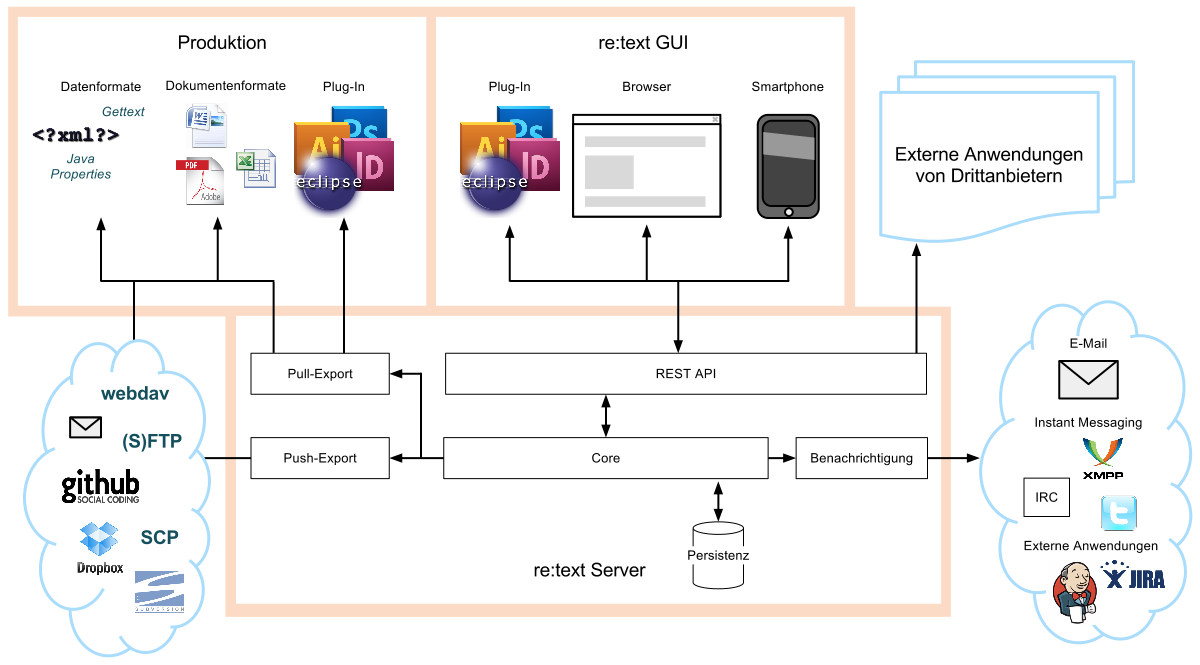
\includegraphics[width=\textwidth]{media/System.pdf}
\caption{Aufbau des Systems}
\label{chart:1}
\end{center}
\end{figure}

Die Zentrale Komponente der Anwendung bildet der Server. Für die Benutzer erfolgt der Zugriff mit Hilfe einer GUI, die mit der REST-API des Servers kommuniziert. In der ersten Version wird eine browserbasierte GUI auf Basis von HTML5 und JavaScript existieren, die auch schon auf Smartphones verwendet werden kann. Später kommen dann spezielle Plugins für Adobe-Produkte und weitere wichtige Produktionsumgebungen hinzu. Auch native GUIs für Smartphones verwenden die gleiche API. Die Schnittstellen können auch von Drittanbietern dazu verwendet werden, eigenen Clients für das System zu entwickeln. In die Endprodukte gelangen die Texten über den Export, exportiert wird dabei in viele Formate, neben Datenformaten wie z.B. XML werden auch Dokumentenformate wie z.B. Word exportiert. Der Export kann durch den Anwender erzeugt werden (\emph{Pull-Export}), aber auch automatisch, z.B. nach festgelegten Zeitplänen oder Ereignissen erfolgen. Dieser \emph{Push-Export} erfolgt auf je nach Projekt festlegbaren Orte, wie z.B. FTP-Server oder Versionsverwaltungssysteme. Die Benachrichtigungen über Aufgaben und Änderungen an Texten kann via E-Mail, aber auch mittels Instant-Messaging-Systeme oder durch den Aufruf fremde API-Endpunkte erfolgen – dies ist ebenfalls innerhalb eines Projektes und pro Nutzer individuell konfigurierbar.

\subsubsection{Grundüberlegung zu einer GUI}

Anforderungen, Grundsätze, Usability, Aufbau, Wireframes

Bei Kontroll-Aufgaben (Lektorat, QS) unterbrechungsfreies Arbeiten ermöglichen (Infinite-Scroll).

Die GUI muss deutlich einfacher zu bedienen sein, als z.B. Word oder Publishing-Systeme, sonst wird sie nicht von Kunden eingesetzt.

\subsection{Zusammenfassung, Nachteile \& Risiken des Konzepts}

In diesem Abschnitt wurde eine Anwendung konzipiert und der darin abgebildetet Workflow beschrieben. Die Konzipierung der Anwendung als Web-Anwendung, bei der alle durchführbaren Operationen über Schnittstellen abgedeckt sind, ermöglicht es, für jeden Mitarbeiter die passenden Zugangswege anzubieten. Als Hauptzugang wird der Webbrowser verwendet, so ist sichergestellt, dass alle Mitarbeiter alle Funktionen des Systems ohne zusätzliche Aufwände wie die Installation neuer Software verwenden können. Für spezielle Anwendungsfällen ist es mit Hilfe der API möglich, Plug-Ins zu entwickeln, die sich in die bevorzugten Werkzeuge der Anwender integrieren.

\paragraph{Nachteile \& Risiken} Ein Nachteil dieses Konzepts liegt in der Zentralisierung der Datenspeicherung. Da alle Daten auf einem zentralen Server verwaltet werden, ist dieser auch der \emph{Single Point of Failure}, d.h. sollte der Server ausfallen, kann kein Mitarbeiter weiterarbeiten. Für einen kommerziellen Betrieb eines solchen Systems ist es also unabdingbar, dass die Server-Infrastruktur ausfallsicher konzipiert ist. 

Das Übertragen der Daten auf einen zentralen Server kann auch zu Bedenken bei den beteiligten Unternehmen führen. Es gibt gerade bei größeren Unternehmen Vorbehalte dagegen, Informationen auf Systemen von Drittanbietern zu speichern. Hier gilt es, genau wie im Hinblick auf die Verfügbarkeit des Systems, einen vertrauenswürdigen Betreiber für die Server-Infrastruktur zu finden. Alternativ ist es jedoch problemlos möglich, das System auch \emph{In-House}, also auf Servern im Unternehmen als \emph{Appliance}, zu betreiben, wobei dann aber zusätzliche Wartungsaufwände entstehen, und damit einige Vorteile des SaaS-Modells ausgehebelt werden. 

Da alle Mitarbeiter über das Internet mit der Anwendung verbunden sind, spielt auch die Bandbreite und Verfügbarkeit einer Internetverbindung eine Rolle. Im Unternehmensbereich spielt dies aber inzwischen nur nur eine untergeordnete Rolle. Trotzdem sollten geeignete Maßnahmen ergriffen werden, die die Arbeit auch mit einer langsamen oder sogar ganz ohne eine Internetverbindung ermöglicht (Offline-Access).

Das größte Risiko dieses Konzeptes ist, dass Mitarbeiter gezwungen werden, sich von ihren bekannten Werkzeugen zu lösen. Gerade bei Mitarbeitern, die vor allem mit Textverarbeitungsprogrammen arbeiten und ansonsten kaum mit anderen Werkzeugen Kontakt haben, wird der Umstieg von der unstrukturierten Arbeitsweise in \trademark{Word} auf die, bis auf den einzelnen Text heruntergebrochene Arbeitsweise in der vorgschlagenen Anwendung, schwer fallen. Man kann aber davon ausgehen, dass für alle Beteiligten die Vorteile der Lösung erkenntlich werden und sich eine Abneigung gegen eine Änderung angestammter Arbeitsabläufe leicht abbauen lässt.



\section{Entwurf des zentralen Systems}\label{l:entwurf}

Im vorigen Kapitel wurde eine Anwendung konzipiert, mit der sich die in Kapitel \ref{l:problemanalyse} · S.\pageref{l:problemanalyse} genannten Probleme beheben lassen. In diesem Kapitel wird ein Prototyp entworfen, der dieses Konzept umsetzt. Mithilfe des Prototyps soll gezeigt werden, dass sich der konzipierte Workflow mit der vorgeschlagenen Anwendungsart -- einer browserbasierte Web-Anwendung mit vollständiger Schnittstellen-Abdeckung -- abbilden lässt und einen Mehrwert für Projekte zur Erstellung von Informations- und Kommunikationsmedienprodukten bietet. 

Der Funktionsumfang des Prototyps ist eingeschränkt, deckt aber die wichtigsten Anforderungen ab. Im Prototyp soll es möglich sein
\begin{itemize}\itemsep -5pt
\item die Struktur eines Produkts zu definieren
\item die Texte des Produkts zu befüllen
\item sich mit anderen Mitarbeitern über die Texte auszutauschen
\item die Texte zu prüfen und freizugeben
\item das Projekt zu exportieren, um die Texte weiterverarbeiten zu können.
\end{itemize}

Die Beschreibungen der Bestandteile der Anwendung in diesem Kapitel gehen zum Teil über diesen Funktionsumfang hinaus, da die Implementierung des Prototyps auch dazu dient, zu zeigen, dass die vorgeschlagene Architektur geignet ist, als Vorlage für eine belastbare Implementierung der Anwendung für den realen Einsatz zu dienen. Der Entwurf liefert hierfür schon wichtige Vorüberlegungen.

\pagebreak

\subsection{Komponenten}

\begin{figure}[htb]
\begin{center}
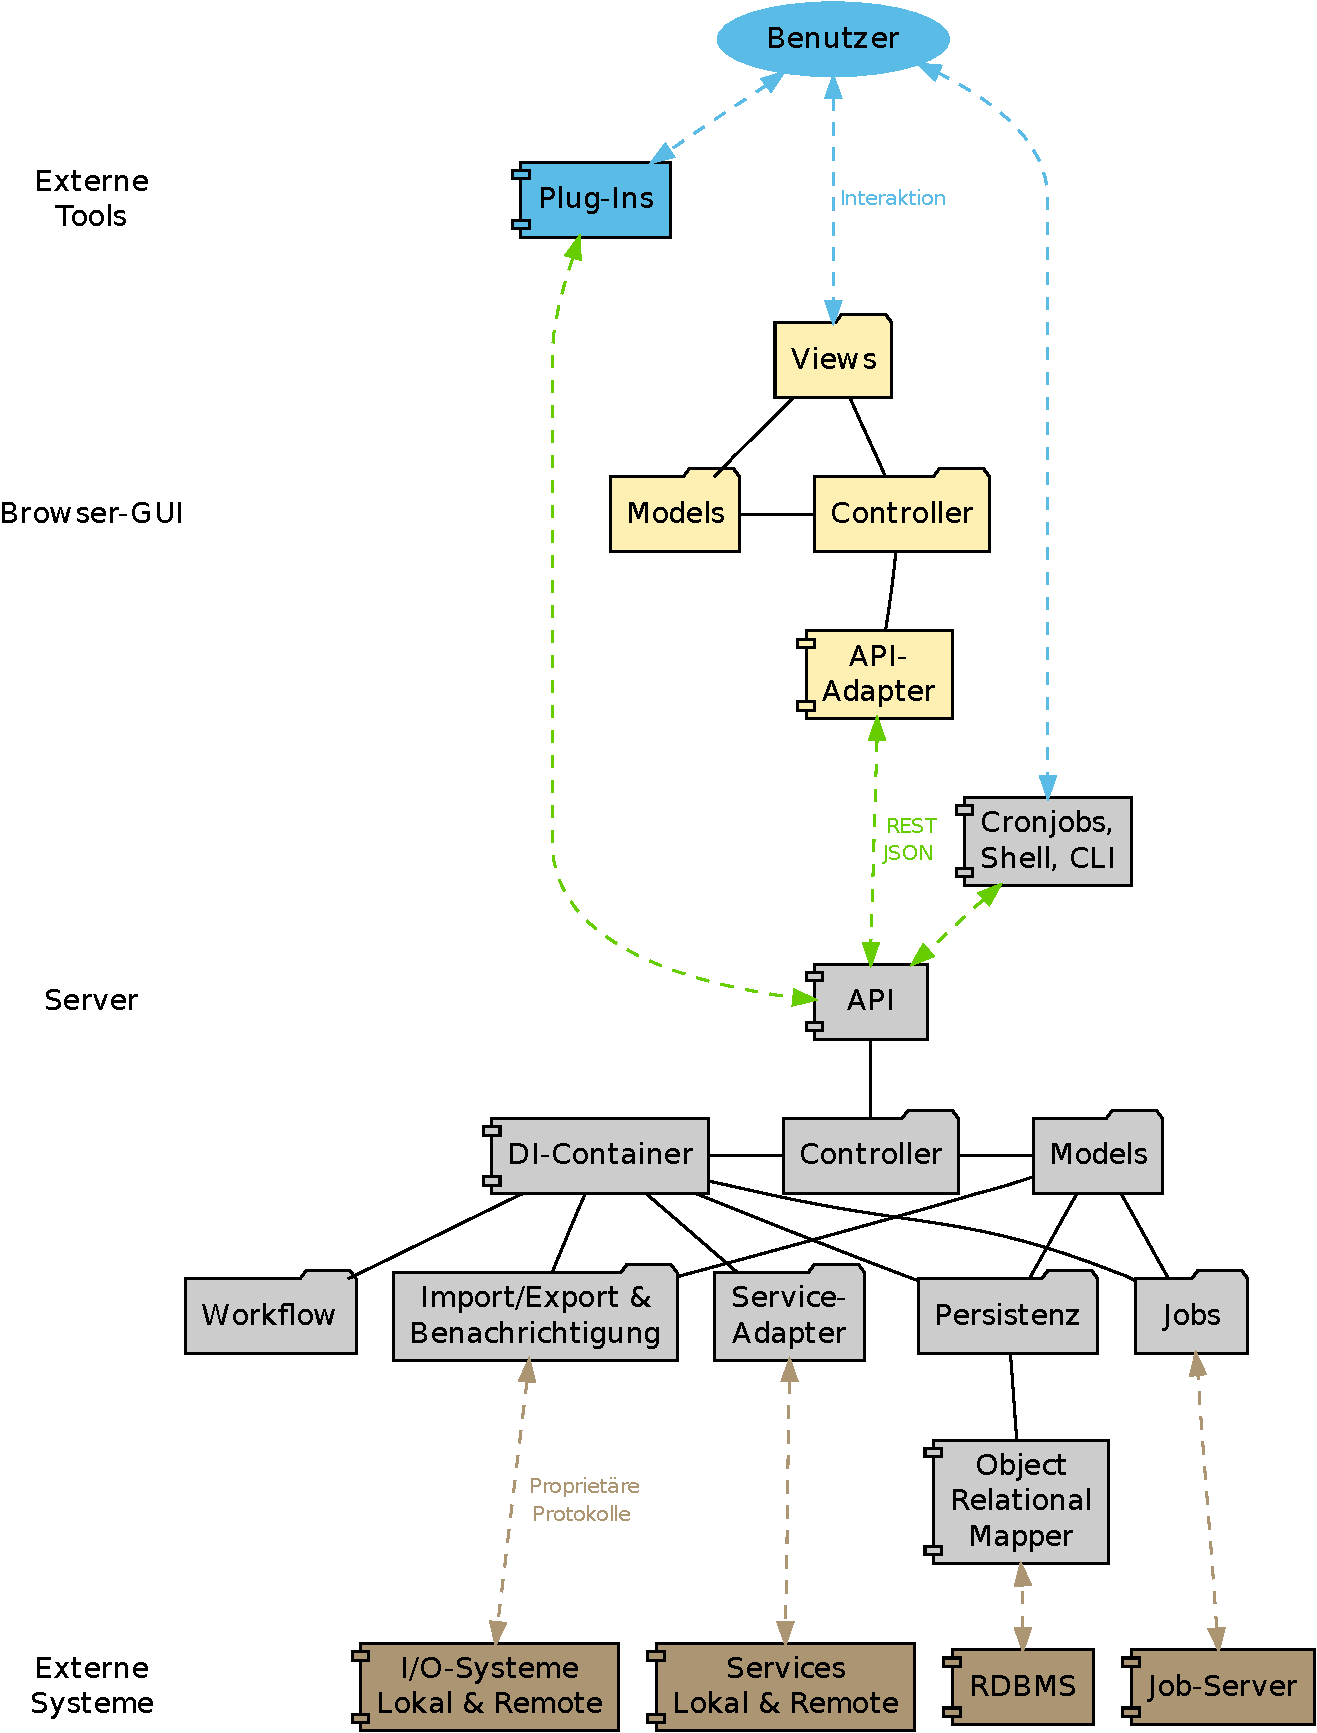
\includegraphics[width=0.75\textwidth]{media/komponenten.pdf}
\end{center}
\caption{Komponententen der Anwendung}
\label{chart:komponenten}
\end{figure}

Abbildung~\ref{chart:komponenten} liefert einen Überblick über die in den folgenden Abschnitten beschriebenen Komponenten der Anwendung. \emph{Blau} eingezeichnet sind der Endanwender und externe Benutzer"=Werkzeuge wie z.B. Plug-Ins und Software von Drittanbietern. \emph{Gelb} eingezeichnet sind die Komponenten des browserbasierten GUI. \emph{Grau} eingezeichnet sind die Komponenten des Anwendungsservers. \emph{Braun} eingezeichnet sind (aus Sicht des Anwendungsservers) externe Dienste, die durch diesen angebunden werden. \emph{Gestrichelte Linien} zeigen Kommunikationsverbindung zwischen Komponenten über Schnittstellen. \emph{Durchgezogene Linien} zeigen Verbindungungen innerhalb eines Systems.

Der zentrale Bestandteil der Anwendung ist der Anwendungsserver, mit dem verschiedene GUIs über Schnittstellen kommunzieren. Das wichtigste GUI ist das browserbasierte Interface, da hiermit alle am Projekt beteiligten Personen arbeiten. Abschnitt \ref{l:entwurf-server} · S.\pageref{l:entwurf-server} beschreibt die Komponenten des Anwendungsserver und Abschnitt \ref{l:entwurf-gui} · S.\pageref{l:entwurf-gui} die Gestaltung des browserbasierten GUIs. In Abschnitt \ref{l:anbindung-gui} · S.\pageref{l:anbindung-gui} wird die Anbindung dieses GUIs an den Anwendungsserver beschrieben.

Zur Validierung des Entwurfes wurde ein Querschnitt durch die vorgestellte Architektur als Prototyp umgesetzt, mit dessen Hilfe sich überprüfen lässt, inwieweit sich das vorgeschlagene Konzept praktisch einsetzen lässt und die entworfene Systemarchitektur geeignet ist, die benötigten Funktionen abzubilden. In Abschnitt \ref{l:implementierung-gui} · S.\pageref{l:implementierung-gui} und \ref{l:implementierung-server} · S.\pageref{l:implementierung-server} wird die prototypische Implementierung der GUI bzw. des Anwendungsservers, die auf dem Entwurf basiert, beschrieben.

Im nächsten Abschnitt wird jedoch zuerst das Domänenmodell, das die gemeinsame Grundlage für GUI und Anwendungsserver bildet, beschrieben.

\pagebreak

\subsection{Domänenmodell}\label{l:domänenmodell}

\begin{center}
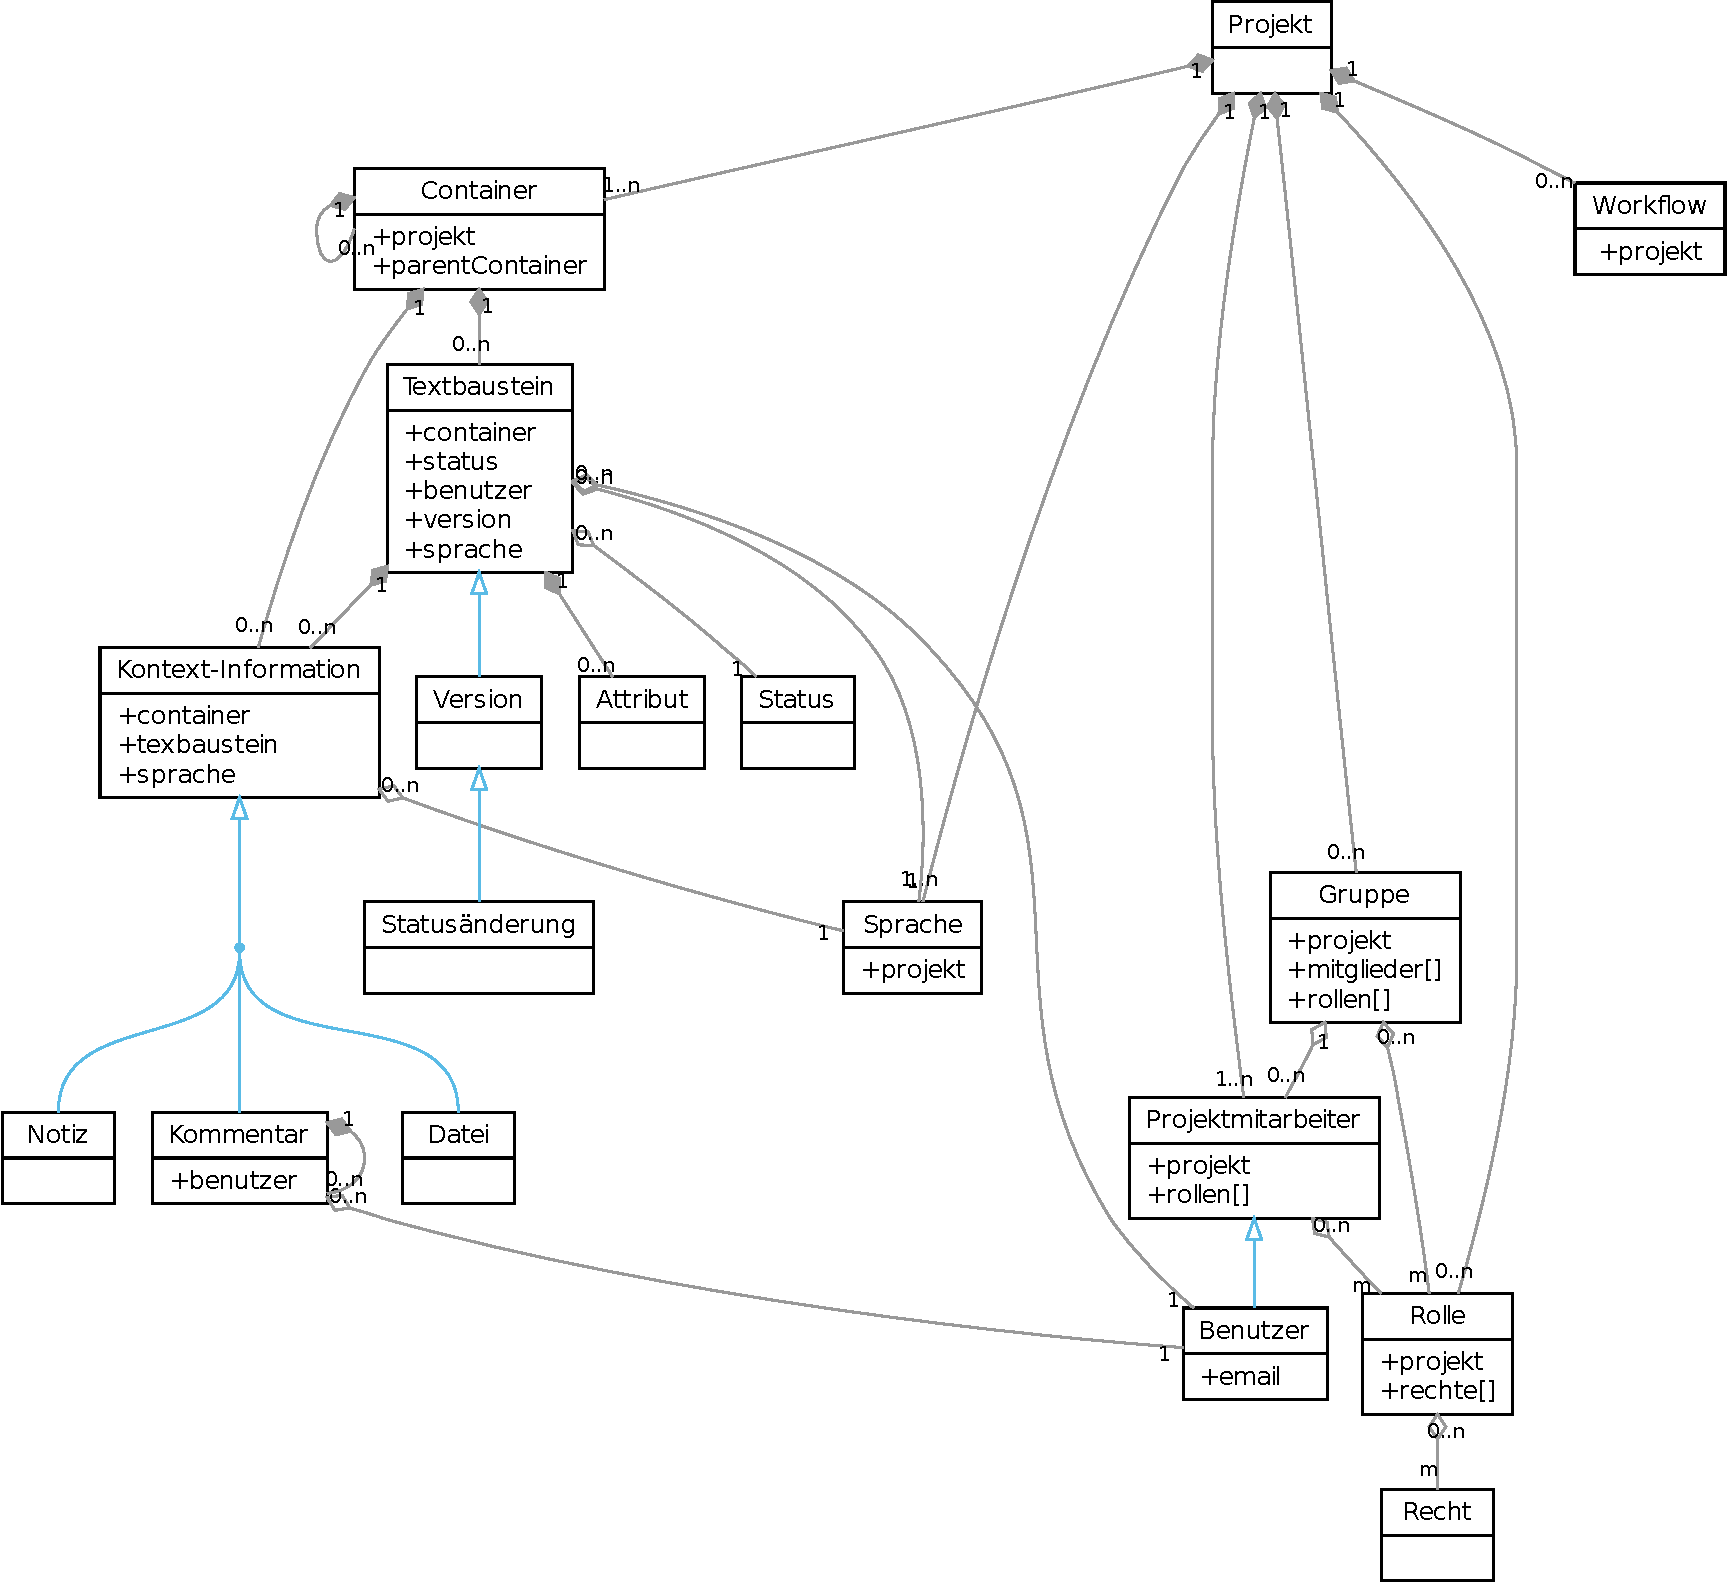
\includegraphics[width=\textwidth]{media/domain.pdf}
\captionof{figure}{Domänenmodell}\label{chart:domain}
\end{center}

Aus den vorangegangenen Überlegungen zur Anwendung und zum Workflow lässt sich ein Domänenmodell extrahieren, das die einzelnen logischen Objekte innerhalb der Anwendung beschreibt. Abbildung~\ref{chart:domain} zeigt das Modell in der Übersicht. Der Entwurf in diesem Kapitel und der Prototyp orientieren sich an diesem Domänenmodell.

Die einzelnen Objekte werden nachfolgend beschrieben:

\textsf{\textbf{Attribut}}\\Beschreibt die Attribute eines Textbausteins.

\textsf{\textbf{Benutzer}}\\Repräsentiert einen Benutzer des Systems.

\textsf{\textbf{Container}}\\Container dienen zur hierarchischen Organisation der Texte innerhalb des Projekts. Container können weitere Container und Texte enthalten. Ein Container ohne übergeordneten Container befindet sich auf der obersten Ebene. Es kann mehrere Container auf der obersten Ebene geben.

\textsf{\textbf{Gruppe}}\\Mitarbeiter können in Gruppen zusammengefasst werden. Dies erleichtert die Konfiguration des Workflows und der Rechte.

\textsf{\textbf{Kommentare}}\\Kommentare enthalten Hinweise und Fragen zu einzelnen Texten und Texbausteinen.

\textsf{\textbf{Kontext-Information}}\\Projektspezifische Kontext-Informationen lassen sich hinterlegen und Textbausteinen und Containern zuordnen.

\textsf{\textbf{Projekt}}\\Projekte bilden den Rahmen für alle Texte eines einzelnen Produkts. Dieses Model geht davon aus, dass auch alle anderen Einstellungen (Gruppenzugehörigkeit, Rechte, Workflows,~…) immer projektspezifisch sind. Dies ist in einem Szenario sinnvoll, in dem unterschiedliche Unternehmen Zugriff auf die selbe Instanz der Anwendung haben. So wird eine saubere Trennung der Daten erreicht.

\textsf{\textbf{Projektmitarbeiter}}\\Gestattet einem Benutzer die Mitarbeit an einem Projekt und legt dabei fest, welche Rechte dem Benutzer für das Projekt zugewiesen sind.

\textsf{\textbf{Recht}}\\Beschreibt das Recht, eine Operation auf einem Objekt auszuführen.

\textsf{\textbf{Rolle}}\\Beschreibt die verschiedenen Rollen innerhalb der Anwendung. Die Rechte der Rollen sind durch die Zuordnung von Benutzern zu Projekten durch den Projektmitarbeiter immer an das jeweilige Projekt gebunden.

\textsf{\textbf{Sprache}}\\Die Texte jedes Projekts liegen in einer oder mehreren Sprachen vor.

\begin{samepage}
\textsf{\textbf{Status}}\\Beschreibt die verschiedenen Zustände eines Textbausteins (vgl. Abschnitt \ref{l:konzept-workflow-status} · S.\pageref{l:konzept-workflow-status}).

\begin{enumerate}\itemsep -5pt
\item \texttt{Neu}, Textbaustein erzeugt
\item \texttt{Leer}, Textbaustein definiert
\item \texttt{Befüllt}, Textbaustein mit Inhalt befüllt
\item \texttt{Korrigiert}, Orthografie geprüft
\item \texttt{Geprüft}, Inhalt geprüft (Qualitätsicherung)
\item \texttt{Freigegeben}, durch Kunden freigegeben
\item \texttt{Veröffentlicht}, in Produkt übernommen
\end{enumerate}
\end{samepage}

\textsf{\textbf{Statusänderung}}\\Beschreibt eine Änderung eines Status durch einen Benutzer, z.B. durch Freigabe oder Überprüfung.

\textsf{\textbf{Textbaustein}}\\Beschreibt einen einzelnen Textbaustein.

\textsf{\textbf{Version}}\\Beschreibt eine Version des Inhalts eines Textbausteins.

\textsf{\textbf{Workflow}}\\Beschreibt einen projektspezifischen Workflow.

\pagebreak

\subsection{Entwurf eines browserbasierten GUI}\label{l:entwurf-gui}

Das browserbasierte GUI der Anwendung ist der wichtigste Zugang zum System, da es von allen Mitarbeitern zu irgendeinem Zeitpunkt verwendet wird. Die Zeit, die der Einzelne damit verbringt kann sich je nach Rolle stark unterscheiden. Neben den sehr unterschiedlichen Anforderungen an das GUI sind die Benutzer auch technisch sehr unterschiedlich stark versiert, wie in den Personas in Kapitel \ref{l:personas} · S.\pageref{l:personas} gezeigt wurde. Diesen Umständen muss bei der Gestaltung Rechnung getragen werden. In Anlehnung an \cite{nielsen} wurden für den Entwurf der browserbasierten GUI folgende Leitlinien gewählt:

\begin{enumerate}\itemsep -5pt
\item Das Wichtigste zuerst: Die aktuelle Aufgabe soll immer im Fokus der Darstellung liegen.
\item Schnell zum Ziel: Alle Aufgaben müssen leicht und unkompliziert durchführbar sein. 
\item Nicht ablenken: Veränderungen in der Darstellung, z.B. durch Benachrichtigungen, lenken ab und müssen deswegen so gestaltet sein, dass diese sich nach den Präferenzen des Nutzers richten.
\item Hilfe nur einen Klick entfernt: Das Hilfesystem muss kontextsensitiv verfügbar sein und ist eine Kernfunktion der Anwendung.
\end{enumerate}

Da die Anwendung von allen Benutzern gerne verwendet werden soll und vor allem die Usability und die Zeitersparnis ein wichtiger Punkt sind, wie man auch skeptische Mitarbeiter überzeugen kann, mit ihren alten Gewohnheiten zu brechen, ist die Beachtung dieser Grundsätze essentiell. Funktionalitäten, die nur von wenigen gebraucht werden, sollten, wenn überhaupt, optional einblendbar sein. Die Konzeption des Systems ermöglicht es leicht, zusätzliche Anwendungen für besondere Benutzergruppen zu schaffen, z.B. Plug-Ins für die speziellen Werkzeuge einzelner Mitarbeiter. Für diese \typoquotes{Power-User} ist dieser Weg meistens der bessere Weg.

Anhand der Personas lässt sich ermitteln, wer und in welchem Umfang das browserbasiert GUI verwenden wird. Tabelle \ref{table:webgui-usage-by-persona} · S.\pageref{table:webgui-usage-by-persona} zeigt in der Übersicht, welche Operationen besonders bei der Entwicklung des GUIs beachtet werden müssen. Besonders viel Zeit werden von Konzeptern und von den Mitarbeitern, die die Inhalte erstellen, kontrollieren und freigeben im GUI verbracht, da diese Tätigkeiten bezogen auf die einzelnen Texte des Produkts sehr arbeitsintensiv sind. In den folgenden Wireframes werden dementsprechend die wichtigsten Ansichten des GUIs beschrieben.

\begin{table}
\begin{center}
\begin{tabular}{@{}l c c c c c c c}
& \textbf{Eva} & \textbf{Lotte} & \textbf{Torsten} &  \textbf{Jorinde} & \textbf{Jan} & \textbf{Arthur} & \textbf{Markus}\\
{\small Operation (vgl.~\ref{l:workflow})} & {\small Konz.} & {\small Des.} & {\small Texter} & {\small Übersetz.} & {\small Prod.} & {\small Projektl.} & {\small Kunde}\\
\hline\\[-1.5ex]
Definieren         & \HarveyFull      & \HarveyQuarter   & \HarveyEmpty    & \HarveyEmpty    & \HarveyEmpty   & \HarveyEmpty     & \HarveyEmpty \\
Schreiben          & \HarveyQuarter   & \HarveyEmpty     & \HarveyFull     & \HarveyFull     & \HarveyEmpty   & \HarveyEmpty     & \HarveyEmpty \\
Korrektur          & \HarveyEmpty     & \HarveyEmpty     & \HarveyHalf     & \HarveyHalf     & \HarveyEmpty   & \HarveyQuarter   & \HarveyQuarter \\
Qualitätskontrolle & \HarveyQuarter   & \HarveyEmpty     & \HarveyEmpty    & \HarveyEmpty    & \HarveyEmpty   & \HarveyFull      & \HarveyHalf \\
Freigabe           & \HarveyEmpty     & \HarveyEmpty     & \HarveyEmpty    & \HarveyEmpty    & \HarveyEmpty   & \HarveyQuarter   & \HarveyQuarter \\
Veröffentlichung   & \HarveyEmpty     & \HarveyEmpty     & \HarveyEmpty    & \HarveyEmpty    & \HarveyQuarter & \HarveyEmpty     & \HarveyEmpty \\
\end{tabular}
\caption[Umfang und Häufigkeit der Benutzung des browserbasierten GUIs bezogen auf die durchgeführte Operation]{Umfang und Häufigkeit der Benutzung des browserbasierten GUIs bezogen auf die durchgeführte Operation\\\begin{tiny}{\HarveyEmpty} selten {\HarveyFull} häufig\end{tiny}}
\label{table:webgui-usage-by-persona}
\end{center}
\end{table}

\pagebreak

\subsubsection{Aufbau des GUIs}\label{l:gui-aufbau}

\begin{center}
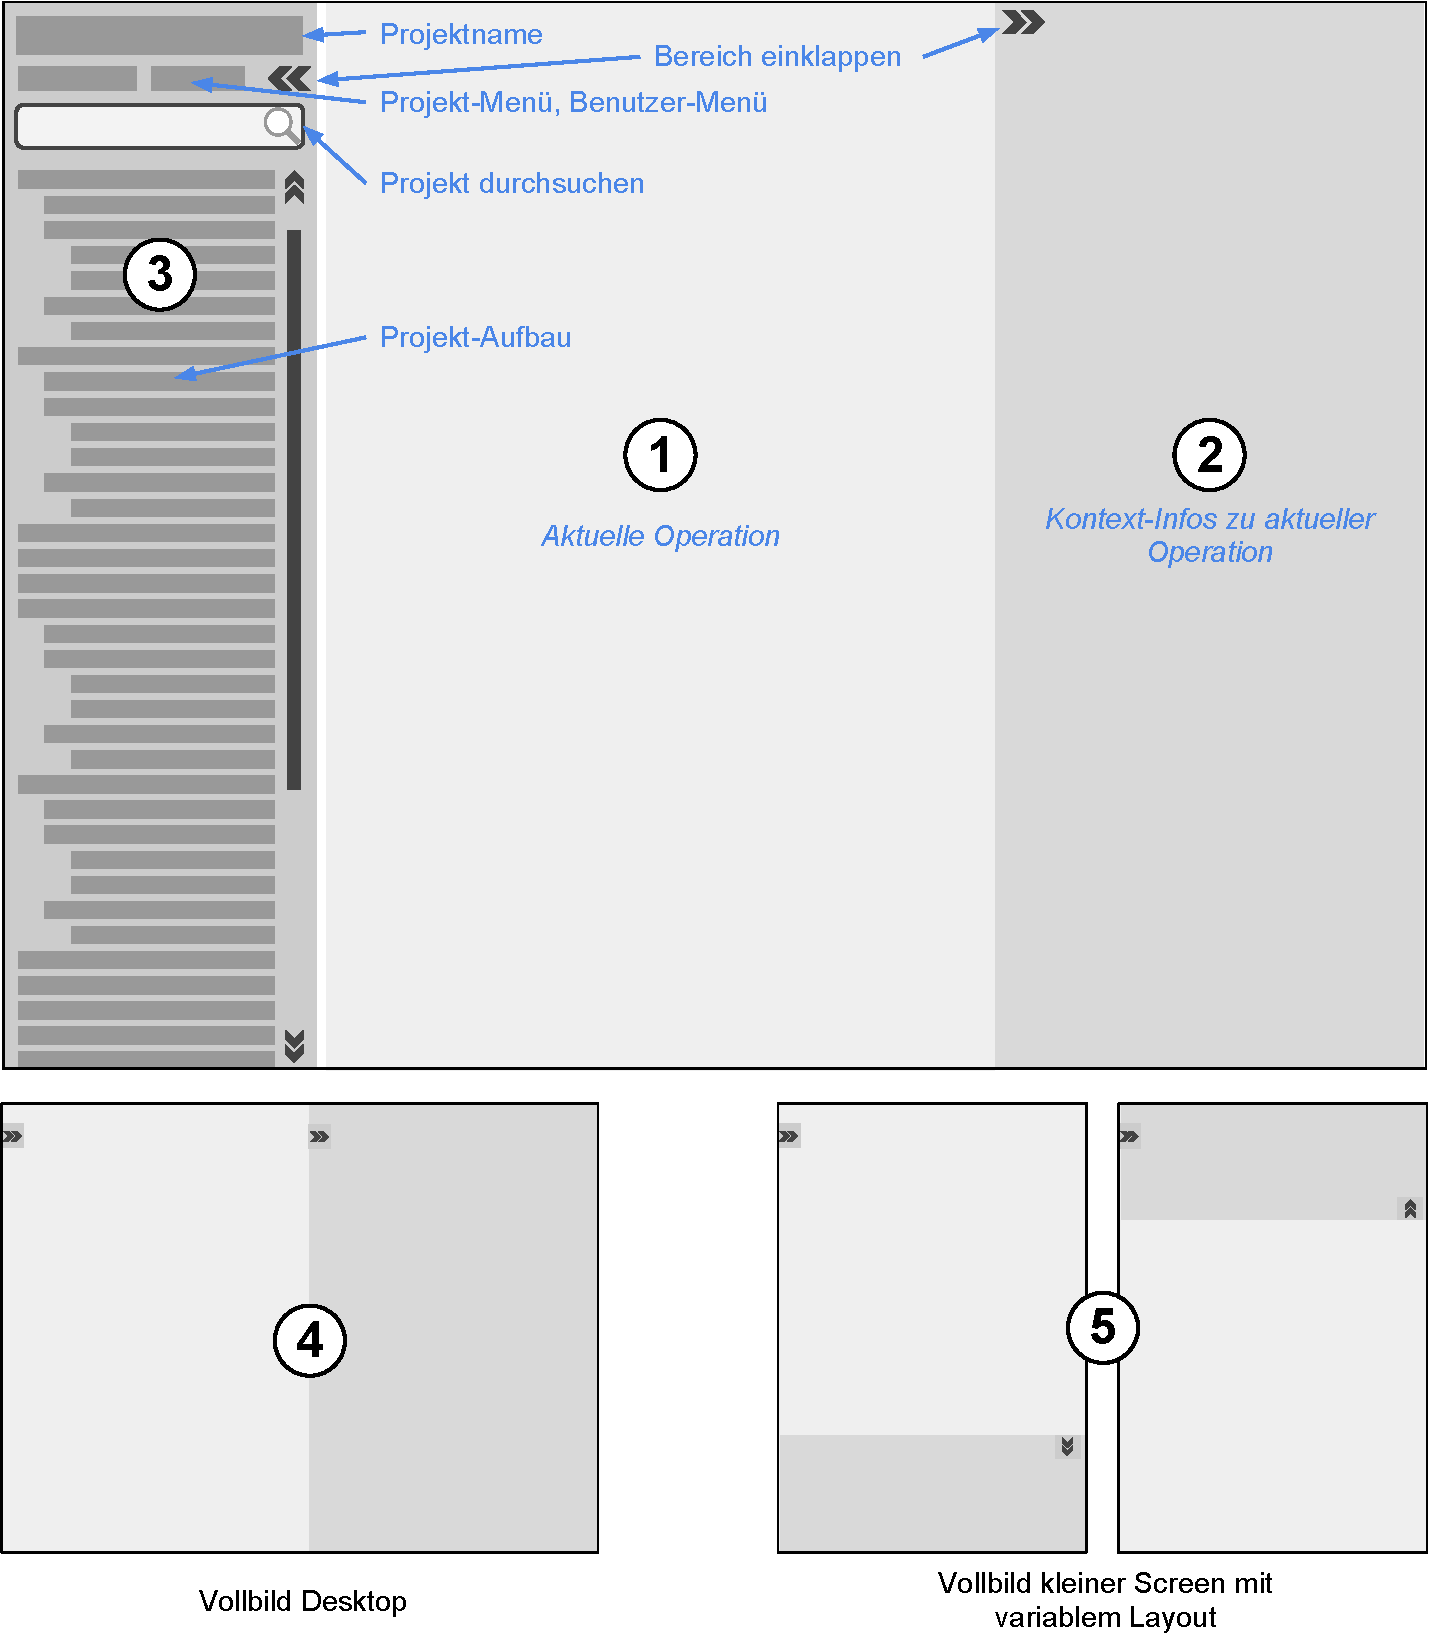
\includegraphics[width=\textwidth]{media/GUIAufbau.pdf}
\captionof{wireframe}{Aufbau des browserbasierten GUIs}\label{chart:gui-aufbau}
\end{center}

Wireframe~\ref{chart:gui-aufbau} zeigt den Grundaufbau des GUIs. Zentraler Bereich ist die Darstellung der \emph{aktuellen Operation} \ball{1} mit den zugehörigen \emph{Kontext-Informationen} \ball{2}. Auf der linken Seite findet sich eine Spalte über die im Projekt navigiert werden kann \ball{3}. Um den Fokus auf die aktuelle Aufgaben zu verbessern, sind die Kontext-Information und die Projektspalte ausblendbar \ball{4}. Das gesamte Layout passt sich flexibel an verschiedene Bildschirmgrößen und -formate an, zusätzlich kann die Position der Kontext-Information an die eigenen Vorlieben angepasst werden \ball{5}.

Die Projekt-Spalte \ball{3} bietet direkten Zugang zu allen Teilen des aktiven Projekts. Die Projektstruktur wird mit einem Navigationsbaum dargestellt, über den direkt zu den jeweiligen Abschnitten gesprungen werden kann. Über das Suchfeld lassen sich die Einträge im Baum filtern. In der Spalte befindet sich oben zur Orientierung der Name des aktiven Projekts. Über das ausklappbare Projektmenü gelangt man zu Ansichten der Anwendung, die nicht direkt über die Texte erreichbar sind, z.B. die Projektauswahl, die Mitarbeiterverwaltung oder den Export. Über das ausklappbare Benutzermenü kann man sich ausloggen, sein Profil bearbeiten und persönliche Einstellungen anpassen.

\pagebreak

\subsubsection{Definieren des Produkts}\label{l:gui-definition}

\begin{center}
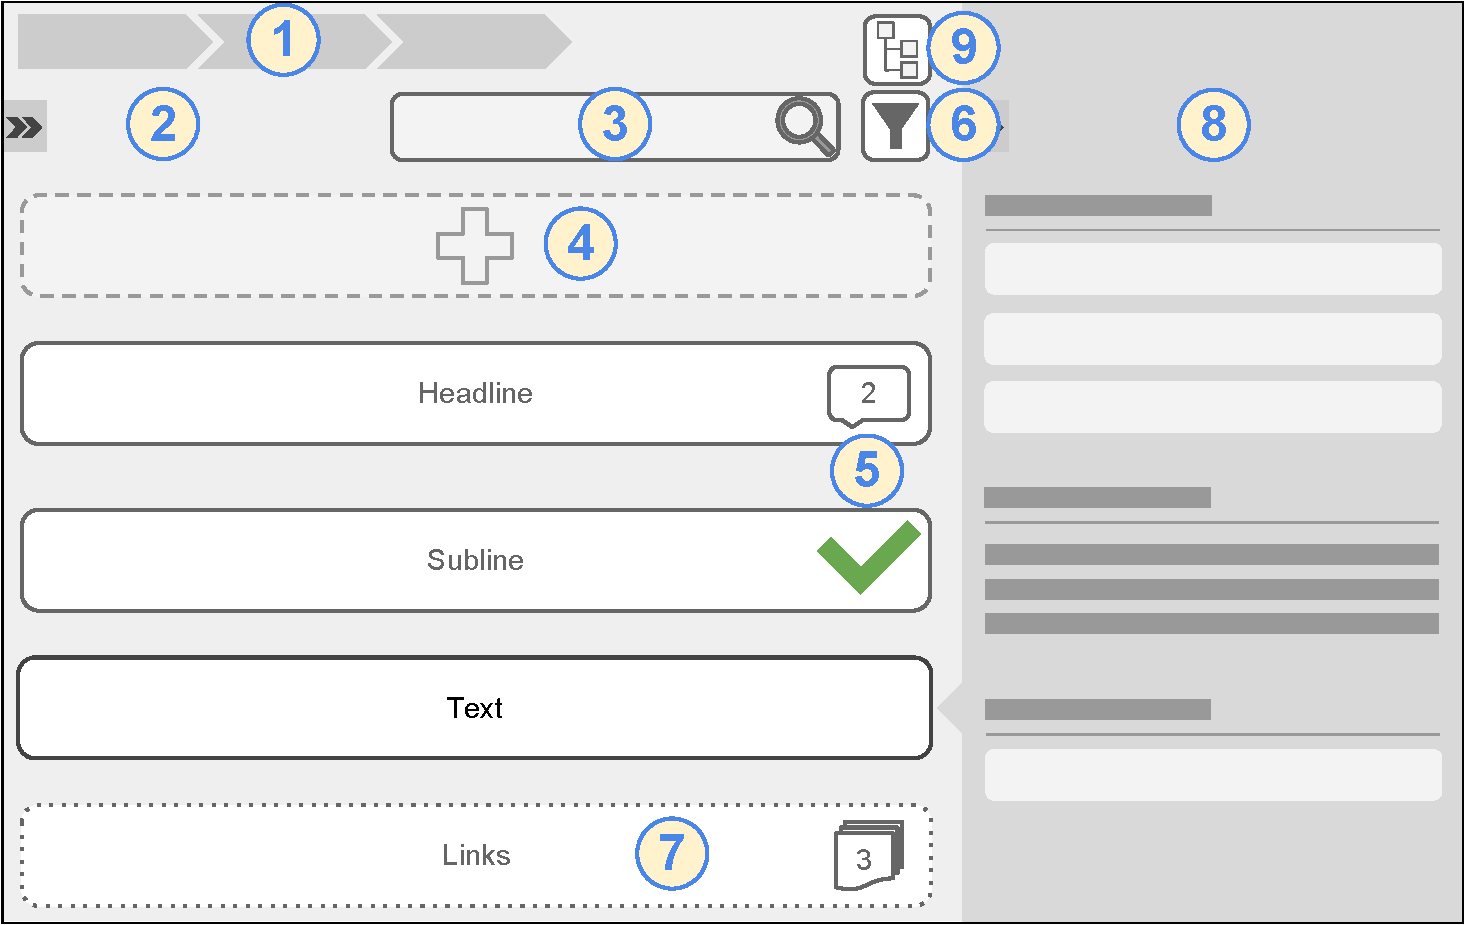
\includegraphics[width=\textwidth]{media/GUIProduktstruktur.pdf}
\captionof{wireframe}{Bearbeiten der Produktstruktur}\label{chart:gui-produktstruktur}
\end{center}

Wireframe~\ref{chart:gui-produktstruktur} zeigt die Darstellung des GUIs zur Bearbeitung der Produktstruktur. Über die Breadcrumb-Navigation \ball{1}, die die aktuelle Position in der Projekthierarchie anzeigt, ist eine Orientierung auch ohne das eingeklappte Projektmenü möglich. Über eine Schaltfläche lassen sich alle Container der aktuellen Hierarchiebene aufklappen, so können umfangreiche Änderungen an vielen Elementen gleichzeitig vorgenommen werden, ohne dass man sich durch die verschiedenen Ebenen \typoquotes{hangeln} muss. Im Inhaltsbereich \ball{2} werden die auf der aktuellen Ebene befindlichen Inhalts-Elemente, Textbausteine und Container, angezeigt. Die Darstellung erfolgt in einer kompakten Weise, die einen schnellen Überblick über die Inhalte bietet ohne viel Scrollen zu müssen. Die einzelnen Inhalts-Elemente können mit Drag\&Drop in ihrer Reihenfolge angepasst werden. Über das Suchfeld \ball{3} können die angezeigten Elemente gefiltert werden. Über eine Schaltfläche \ball{4} können neue Inhalts-Elemente erstellt werden. Zusatzinformationen wie der Typ, der Status, Kommentare oder ähnliche können auch verwendet werden, um die Inhalte in der Ansicht zu filtern, z.B. um nur die Elemente anzuzeigen, für die noch die Inhalte fehlen \ball{5}. Durch Klick auf einen Container \ball{6} gelangt man eine Ebene tiefer, in diesen Container hinein. Das Icon gibt die Anzahl der untergeordneten Elemente an. In der Spalte für die Kontext-Information \ball{7} werden Detailinformationen zum aktuell ausgewählten Element dargestellt, die an die eingestellte Ansichts-Art angepasst sind. Hier findet sich auch die Bearbeitungshistorie und die Kommentare zu den Inhalts-Elementen.

Über eine Schaltfläche \ball{8} kann zwischen den vier Ansichten (Definieren~·~\ref{l:gui-definition}, Erstellen~·~\ref{l:gui-texten}, Übersetzen~·~\ref{l:gui-uebersetzen} und Prüfen~·~\ref{l:gui-qs}), die die Inhaltselemente manipulieren, gewechselt werden.

\pagebreak

\subsubsection{Texte erstellen}\label{l:gui-texten}

\begin{center}
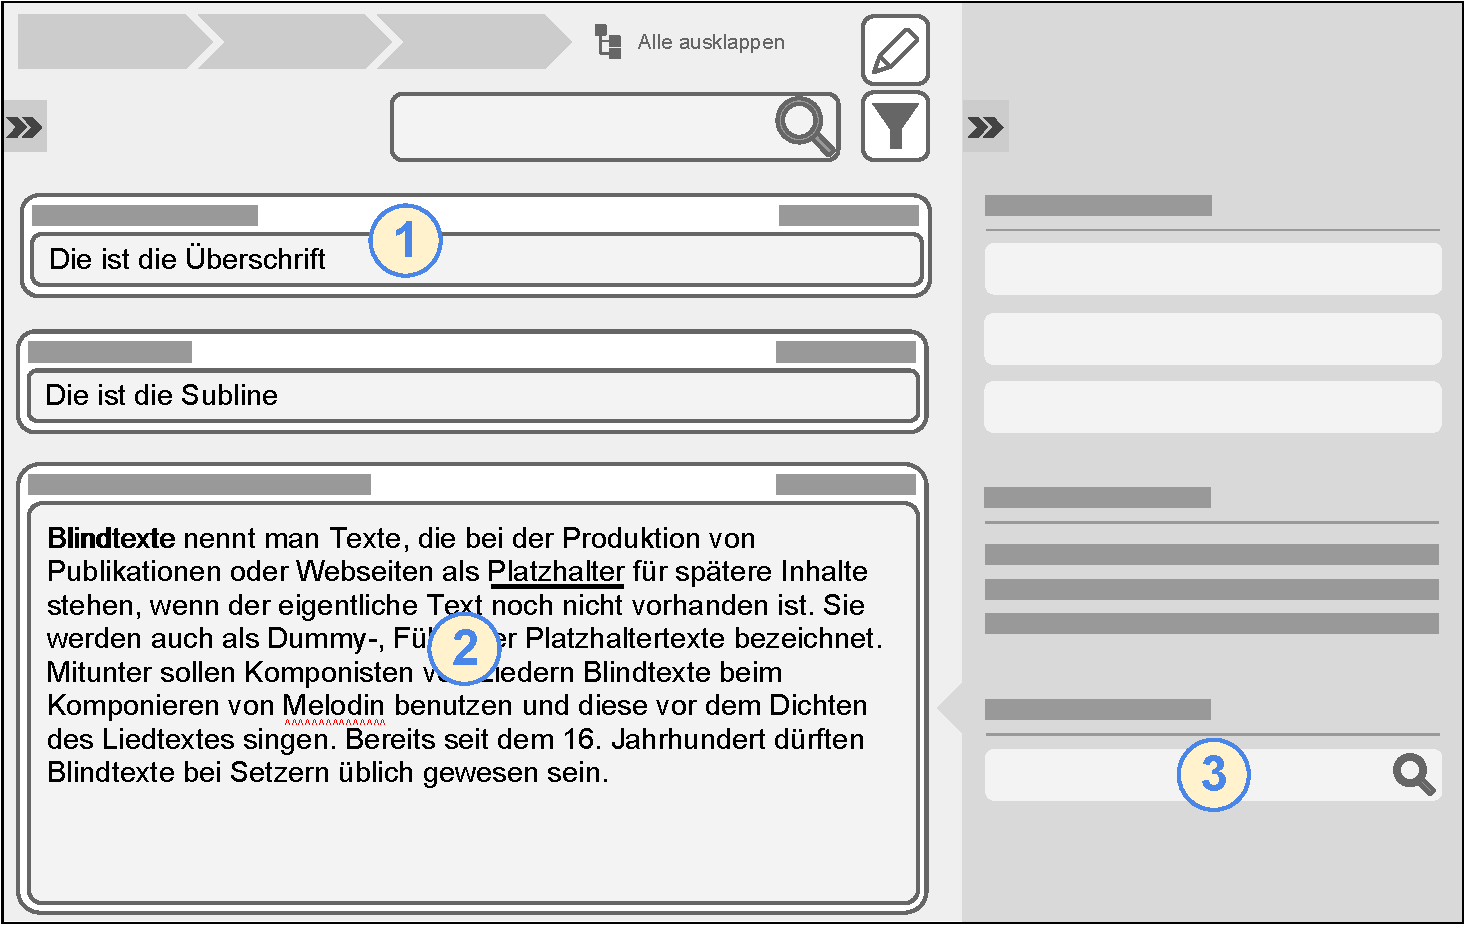
\includegraphics[width=\textwidth]{media/GUITexteerstellen.pdf}
\captionof{wireframe}{Erstellen der Texte}\label{chart:gui-texten}
\end{center}

Wireframe~\ref{chart:gui-texten} zeigt die Darstellung des GUIs zur Bearbeitung der Texte des Produkts. Die Inhaltselemente in der aktuelle Hierarchie werden dabei mit Eingabefeldern für die Inhalte dargestellt \ball{1}. Links über dem Eingabefeld wird die Bezeichnung des Textbausteins angezeigt und rechts darüber Hinweise zu Längebeschränkungen (falls vorhanden) mit entsprechendem Zähler. Während der Eingabe können bereits Auszeichnungen vorgenommen werden, die Schaltflächen dazu werden eingeblendet, sobald sich der Cursor im Feld befindet. Innerhalb der Kontext-Informationen \ball{3} besteht die Möglichkeit direkt eine Suche zu starten, die Suchergebnisse werden in einem Dialog-Fenster geöffnet.

\pagebreak

\subsubsection{Texte übersetzen}\label{l:gui-uebersetzen}

\begin{center}
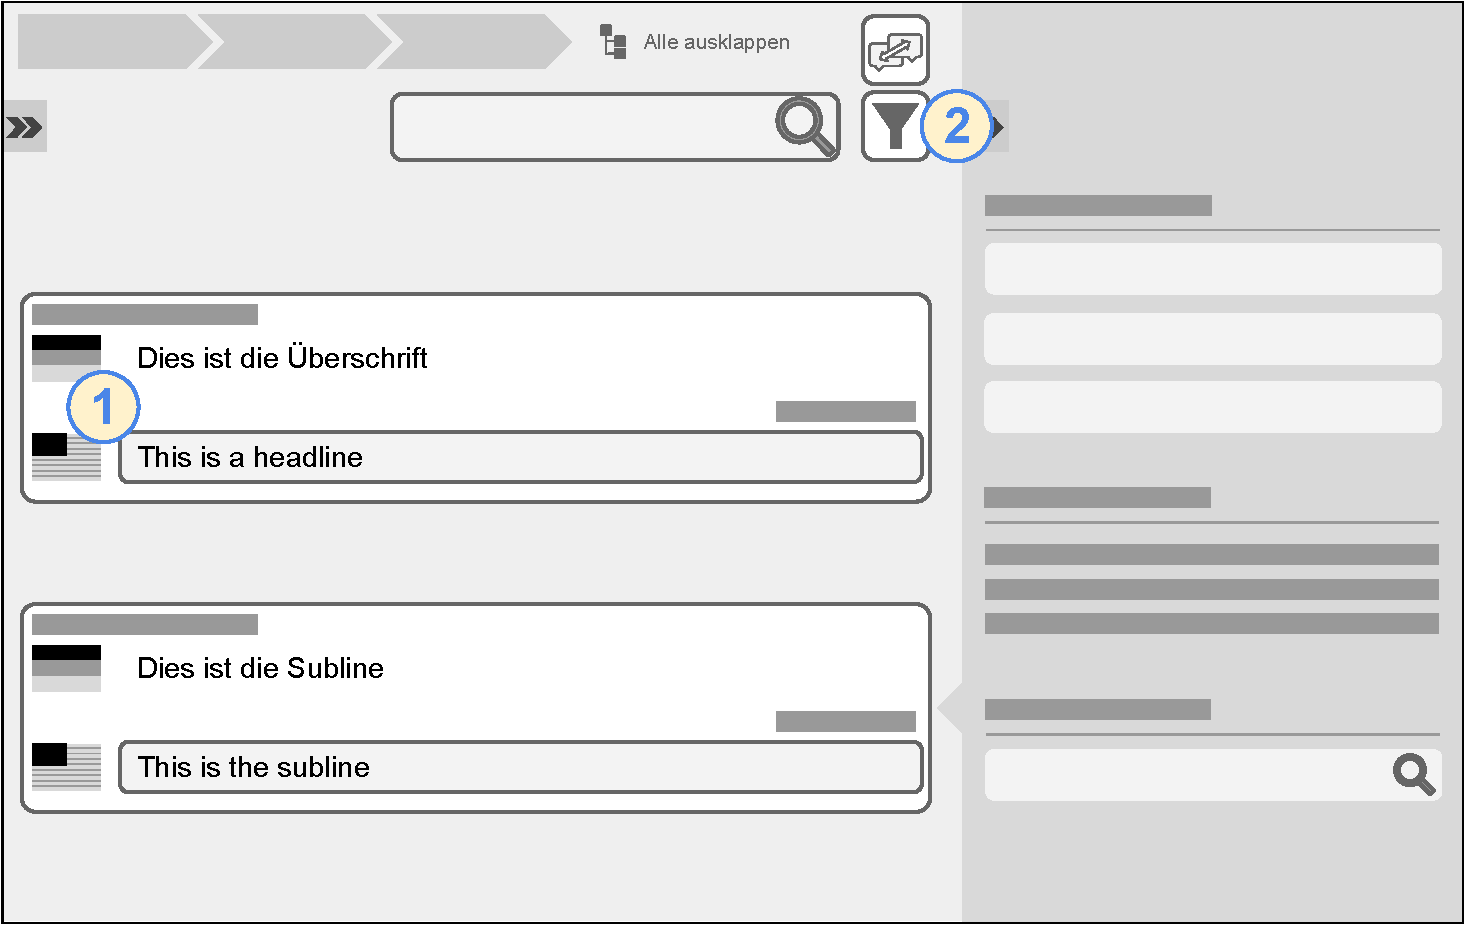
\includegraphics[width=\textwidth]{media/GUITexteuebersetzen.pdf}
\captionof{wireframe}{Übersetzen der Texte}\label{chart:gui-uebersetzen}
\end{center}

Wireframe~\ref{chart:gui-uebersetzen} zeigt die Darstellung des GUIs zur Übersetzung der Texte des Produkts. Hierzu wird der Inhalt des Textbausteins in der Original-Sprache angezeigt und darunter ein Eingabefeld, in dem die Übersetzung eingetragen wird \ball{1}. Über einen Filter-Dialog \ball{2} kann konfiguriert werden, welche Sprachen angezeigt werden sollen.

\pagebreak

\subsubsection{Prüfen}\label{l:gui-qs}

\begin{center}
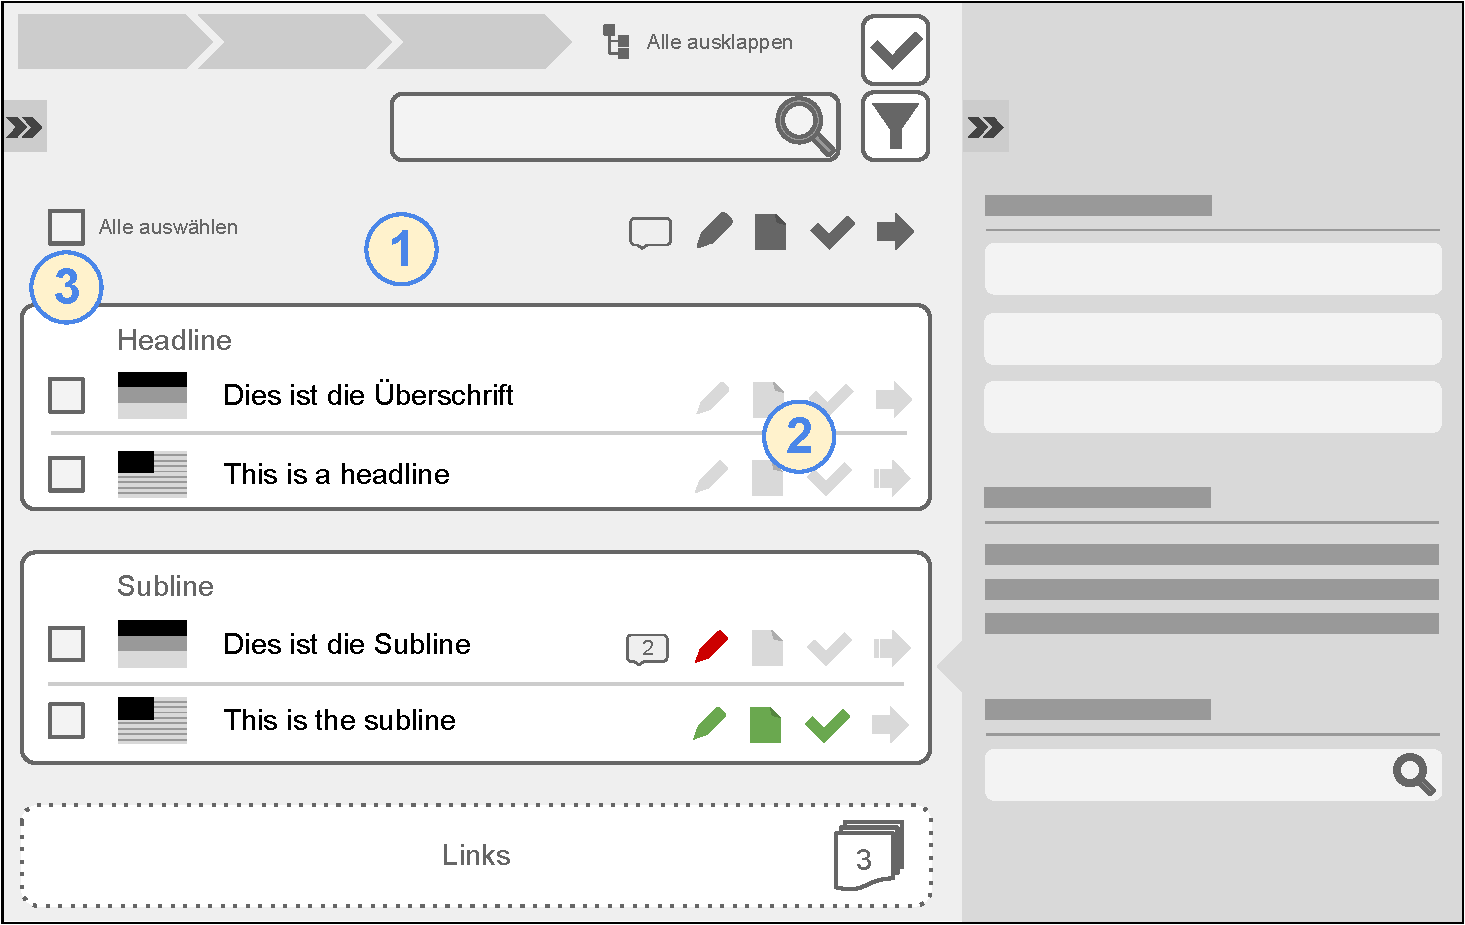
\includegraphics[width=\textwidth]{media/GUIFreigabe.pdf}
\captionof{wireframe}{Überprüfen der Texte}\label{chart:gui-qs}
\end{center}

Wireframe~\ref{chart:gui-qs} zeigt die Darstellung des GUIs zur Kontrolle und Freigabe der Texte des Produkts. In dieser Ansicht werden die verschiedenen Status der Textbausteine bearbeitet. Hierzu sind die Textbausteine mit ihren Übersetzungen dargestellt \ball{1}. Über die mit Icons markierten Schaltflächen \ball{2} lassen sich die einzelnen Status direkt setzen. Von links nach rechts sind das: Korrigiert, Geprüft, Freigegeben und Veröffentlicht. Es wird jeweils zwischen \typoquotes{keine Angabe} (grau), \typoquotes{abgelehnt} (rot) und \typoquotes{in Ordnung} (grün) unterschieden. Hier wird auch die Anzahl der hinterlegten Kommentare angezeigt. Zum massenhaften Bearbeiten von Status können mehrere oder alle Elemente über die Checkboxen \ball{3} ausgewählt werden. Über die Status-Icons in der Kopfzeile kann dann der Status für alle ausgewählten Elemente gleichzeitig gesetzt werden.

\pagebreak

\subsubsection{Kontext-Informationen}\label{l:gui-kontext}

\begin{center}
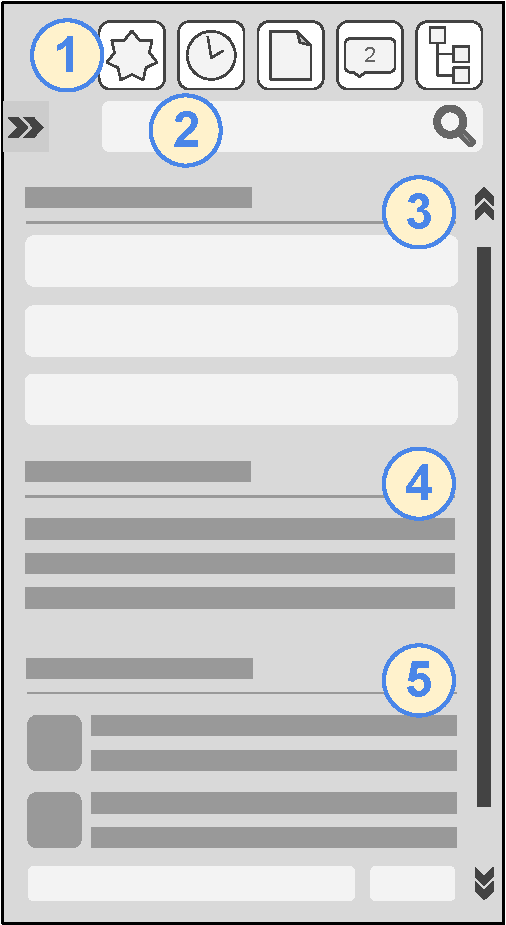
\includegraphics[width=0.35\textwidth]{media/GUIKontext-Informationen.pdf}
\captionof{wireframe}{Kontext-Informationen}\label{chart:gui-kontext}
\end{center}

Wireframe~\ref{chart:gui-kontext} zeigt die Darstellung des GUIs zur Anzeige und Bearbeitung der Kon"-text-In"-for"-ma"-ti"-on"-en. Der Inhalt der Ansicht ist an die jeweilige Operation angepasst. Im oberen Bereich kann zwischen verschiedenen Kontextinformationen zu dem jeweiligen Inhalt umgeschaltet werden \ball{1} (v.l.n.r): 

\begin{enumerate}\itemsep -5pt
\item Neues: Listet die neuesten Informationen aus den vier Bereichen und den aktuellen Status auf.
\item Änderungshistorie: Anzeige der vergangenen Änderungen, mit der Möglichkeit, diese zu kommentieren und zurückzunehmen.
\item Material: Zeigt hinterlegte Materialien an. Dabei handelt es sich um Dateien und Freitext-Notizen.
\item Kommentare: Zeigt die Kommentare an.
\item Struktur: Zeigt Informationen zur Struktur innerhalb des Produkts, wie z.B. die Attribute, an.
\end{enumerate}

Über das Suchfeld \ball{2} lässt sich die aktuelle Ansicht filtern. In der Kontextinformation findet sich direkter Zugang zu Informationen und Operationen bezogen auf den aktuellen Inhalt. Die Inhalte lassen sich über Formulare \ball{3} direkt bearbeiten, Notizen und Dateien werden angezeigt \ball{4} und die Diskussion mithilfe der Kommentarfunktion ist möglich \ball{5}.

\pagebreak

\secbar

Die in diesem Abschnitt gezeigten Wireframes sind die Vorlage für eine mögliche Implementierung. Bei der Umsetzung des Protypen wurde versucht, dieser Vorlage weitestgehend zu folgen, wie in Abschnitt \ref{l:implementierung-gui} · S.\pageref{l:implementierung-gui} beschrieben wird. Im nächsten Abschnitt wird jedoch zuerst auf die Verbindung des Anwendungsservers mit einem GUI eingegangen.

\pagebreak

\subsection{Anbindung des GUI an den Anwendungsserver}\label{l:anbindung-gui}

Die in Abbildung~\ref{chart:komponenten} · S.\pageref{chart:komponenten} \emph{gelb} eingezeichneten Komponenten zeigen den Aufbau eines browserbasierten GUIs. Mittlerweile ist es üblich, klassische Paradigmen aus der Softwarentwicklung auch in browserbasierten Anwendung zu verwenden. Dementsprechend wird die GUI in Form einer MVC-Anwendung implementiert. Die Kommunikation mit dem Anwendungsserver wird in einer eigenen Komponente, dem \emph{API-Adapter}, gekapselt, die über die RESTful"=Schnittstelle JSON-Daten mit dem Anwendungsserver austauscht. Die Repräsentation der Domänendaten erfolgt dabei mithilfe von entsprechenden \emph{Models}, die durch die \emph{Controller} mit den \emph{Views} verbunden werden. Die Models sind nicht zwangsläufig mit den Models auf der Serverseite identisch sondern können Aggregationen sein, oder nur Teile der Daten abbilden. Sie orientieren sich an der öffentlichen API des Anwendungsserver, die nicht zwingenderweise die internen Models 1:1 nach außen weiterreicht. Views sind einzelne Bestandteile einer Ansicht. So lassen sich individuelle Bereiche der Darstellung leicht aktualisieren, ohne die ganze Seite neu laden zu müssen -- in \cite[S.1--5 und S.65--72]{maccaw2011javascript} ist dieses Prinzip ausführlich erläutert.

Ein Problem beim Datenaustausch mithilfe von JSON-Objekten ist, dass diese üblicherweise nur reine Daten enthalten, da schlichterweise Objekte serialisiert werden. Beim Serialisieren werden dann nur die Eigenschaften einer Objekt-Instanz beibehalten, Informationen wie die Klasse oder Relationen zu anderen Objekten werden verworfen. Werden APIs nach diesem Schema verwendet, müssen die Entwickler wissen, hinter welchem Endpunkt sie welche Arten von Daten erwarten. Diese Information wird als Quellcode in der Anwendung hart kodiert. Um zukünftigen Änderungen an der Schnittstelle ohne Änderungen auf Clientseite begegnen zu können, sollten die Antworten der Schnittstelle mit Meta-Informationen versehen sein, die es dem Client ermöglichen, ohne hart kodierte Zuordnung zwischen Endpunkt und Domänenobjekt auszukommen. 

\begin{samepage}
\trademark{JSON-LD}\footnote{\url{http://json-ld.org/}} hat sich dabei als Lösung bewährt. Hierbei werden JSON-Objekt mit Me"-ta-In"-for"-mat"-ion"-en versehen, die beschreiben, um \emph{was} für ein Objekt es sich bei der Antwort handelt (\texttt{@context}) und um \emph{welches} (\texttt{@id}):

\begin{verbatim}
{ "@context": "http://json-ld.org/contexts/person.jsonld",
  "@id": "http://dbpedia.org/resource/John_Lennon",
  "name": "John Lennon",
  "born": "1940-10-09",
  "spouse": "http://dbpedia.org/resource/Cynthia_Lennon" }
\end{verbatim}
\end{samepage}

In dieser Art kann ein JSON-Objekt auch mit Informationen über zugehörige \emph{andere} Objekte versehen werden. Im Beispiel verweist \texttt{spouse} auf die URL unter der das JSON-Objekt der Ehefrau abgerufen werden kann. Auf diese Weise lässt sich die vollständige Datenstruktur einer Anwendung als Graph darstellen. Hierzu werden alle Objekte mit Relationen annotiert und der Client kann entscheiden, welchen Relationen er folgt und welchen nicht. Da die Relations-Informationen auch die URLs zu den Endpunkten enthalten, müssen in der Implementierung keine Endpunkte mehr hart codiert werden, es ist lediglich nötig, einen Einstiegs-Punkt zu kennen von dem aus man mit sich durch den Graphen \typoquotes{hangeln} kann, indem man Objekt-Relationen folgt, deren Kontexte die Anwendung erkennt.\footnote{\url{http://coderbyheart.de/blog/relationen-in-linked-data}}

\pagebreak

\subsection{Implementierung des GUI}\label{l:implementierung-gui}

Im Prototyp wurden das GUI als reine JavaScript-Anwendung umgesetzt. Als Framework für den Aufbau der Anwendung wurde \trademark{Backbone.js}\footnote{\url{http://backbonejs.org/}} eingesetzt. 

\subsubsection{Komponenten}

\trademark{Backbone.js} stellt Basisklassen für Models, Views und Collections (Listen von Models) zur Verfügung, die mithilfe eines zentralen Routers zu einer Anwendung verbunden werden können, die mit einer RESTful-API kommunziert. Der Router übernimmt dabei die Aufgabe, abhängig von der URL im Browser zu steuern, welche View gerade eingezeigt wird. 

Um die einzelnen Bestandteile der Anwendung möglichst modular und die Ladezeiten so kurz wie möglich zu halten, kommt \trademark{require.js}\footnote{\url{http://requirejs.org/}} zum Einsatz, mit dessen Hilfe es möglich ist, nur die für den aktuellen Code-Pfad nötigen Abhängigkeiten zu laden. Neben dem Nachladen von Ja\-va\-Scr\-ipt-Code ist es damit auch möglich HTML-Dateien nachzuladen, dies wird in der Implementierung dazu verwendet, den HTML-Code zur Darstellung der Anwendung ebenfalls modular und nur bei Bedarf nachzuladen. Dies ermöglich zudem eine saubere Trennung zwischen der Darstellungslogik, die in JavaScript implementiert ist und dem zugehörigen HTML-Quellcode. \trademark{Underscore.js}\footnote{\url{http://underscore.org/}}, auf dem \trademark{Backbone.js} aufbaut, liefert hierzu einfache Templating-Funktionen.

Zur Realisierung der GUI-Funktionalität wurde \trademark{Twitter Bootstrap}\footnote{\url{http://twitter.github.com/bootstrap/}} eingesetzt, ein HTML5-Framework, das für viele GUI-Elemente bereits vorgefertigte Darstellungen bietet. Einige Elemente werden mithilfe von JavaScript mit erweiterter Funktionalität versehen, in \trademark{Twitter Bootstrap} kommt dabei \trademark{JQuery}\footnote{\url{http://jquery.com/}} zum Einsatz. \trademark{Twitter Bootstrap} ermöglich von sich aus das GUI \emph{responsive} zu implementieren, d.h. dass keine festen Maßangaben verwendet werden. So ist eine saubere Darstellung auf vielen unterschiedlichen Endgeräten sichergestellt. Mithilfe von \emph{CSS media queries} können einfach Anpassung für bestimmte Bildschirmgrößen implementiert werden.

Alle genannten Komponenten sind umfangreich getestet, funktionieren in allen aktuellen Browsern und sind auch abwärtskompatibel zu älteren Browsern.

\setlength\fboxsep{2pt}
\setlength\fboxrule{0.5pt}

\begin{center}
\fbox{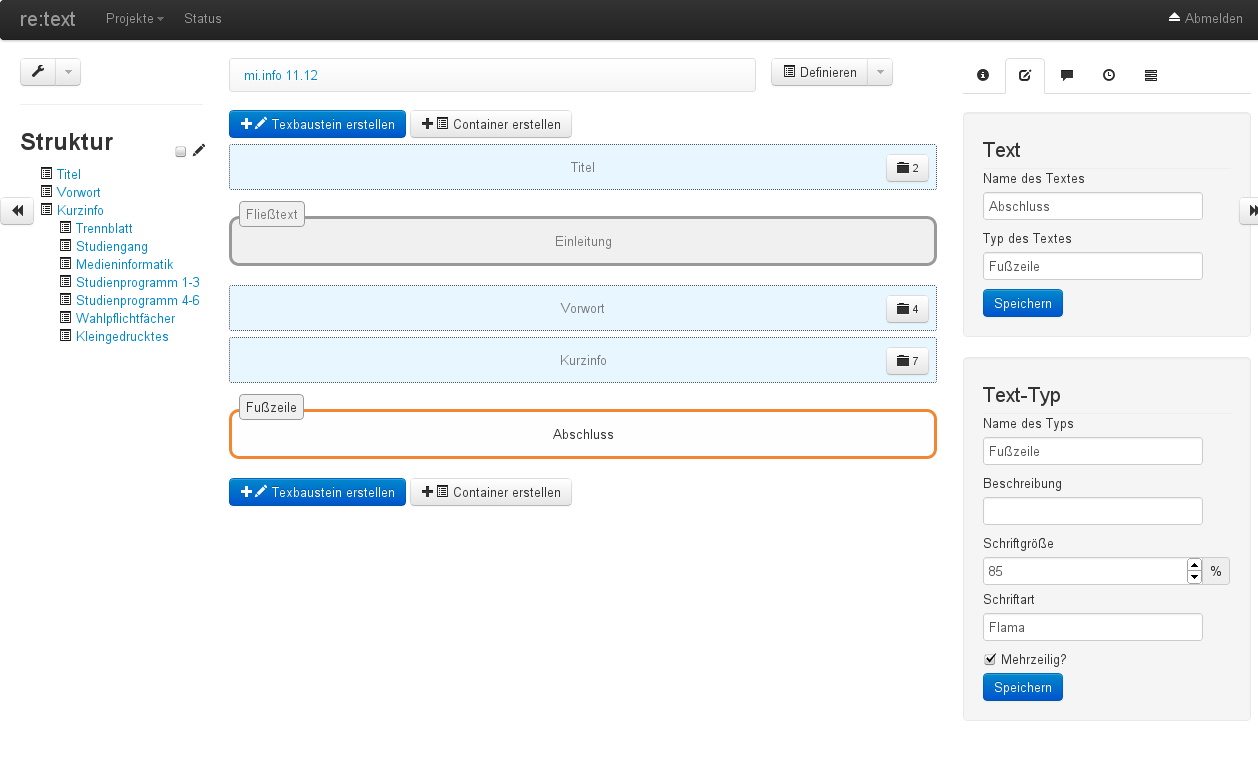
\includegraphics[width=\textwidth]{media/screenshots/app.png}}
\captionof{screenshot}[Browserbasiertes GUI des Prototyps]{Browserbasiertes GUI des Prototyps (vgl. Abschnitt \ref{l:gui-definition} · S.\pageref{l:gui-definition})}\label{chart:gui-prototyp}
\end{center}

Screenshot~\ref{chart:gui-prototyp} zeigt den Aufbau des GUI des Prototyps beispielhaft in der Ansicht zur Definition des Produkts. Die Anordnung der Elemente des Entwurfs wurde weitgehend beibehalten. Unterschiede resultieren aus im Prototyp nicht implementierte Funktionen, die nicht mit Platzhalter-Elementen dargestellt werden, sondern entfallen. Weitere Screenshots finden sich in Anhang~\ref{l:screenshots} · S.\pageref{l:screenshots}.

\subsubsection{Klassendiagramm}

\begin{center}
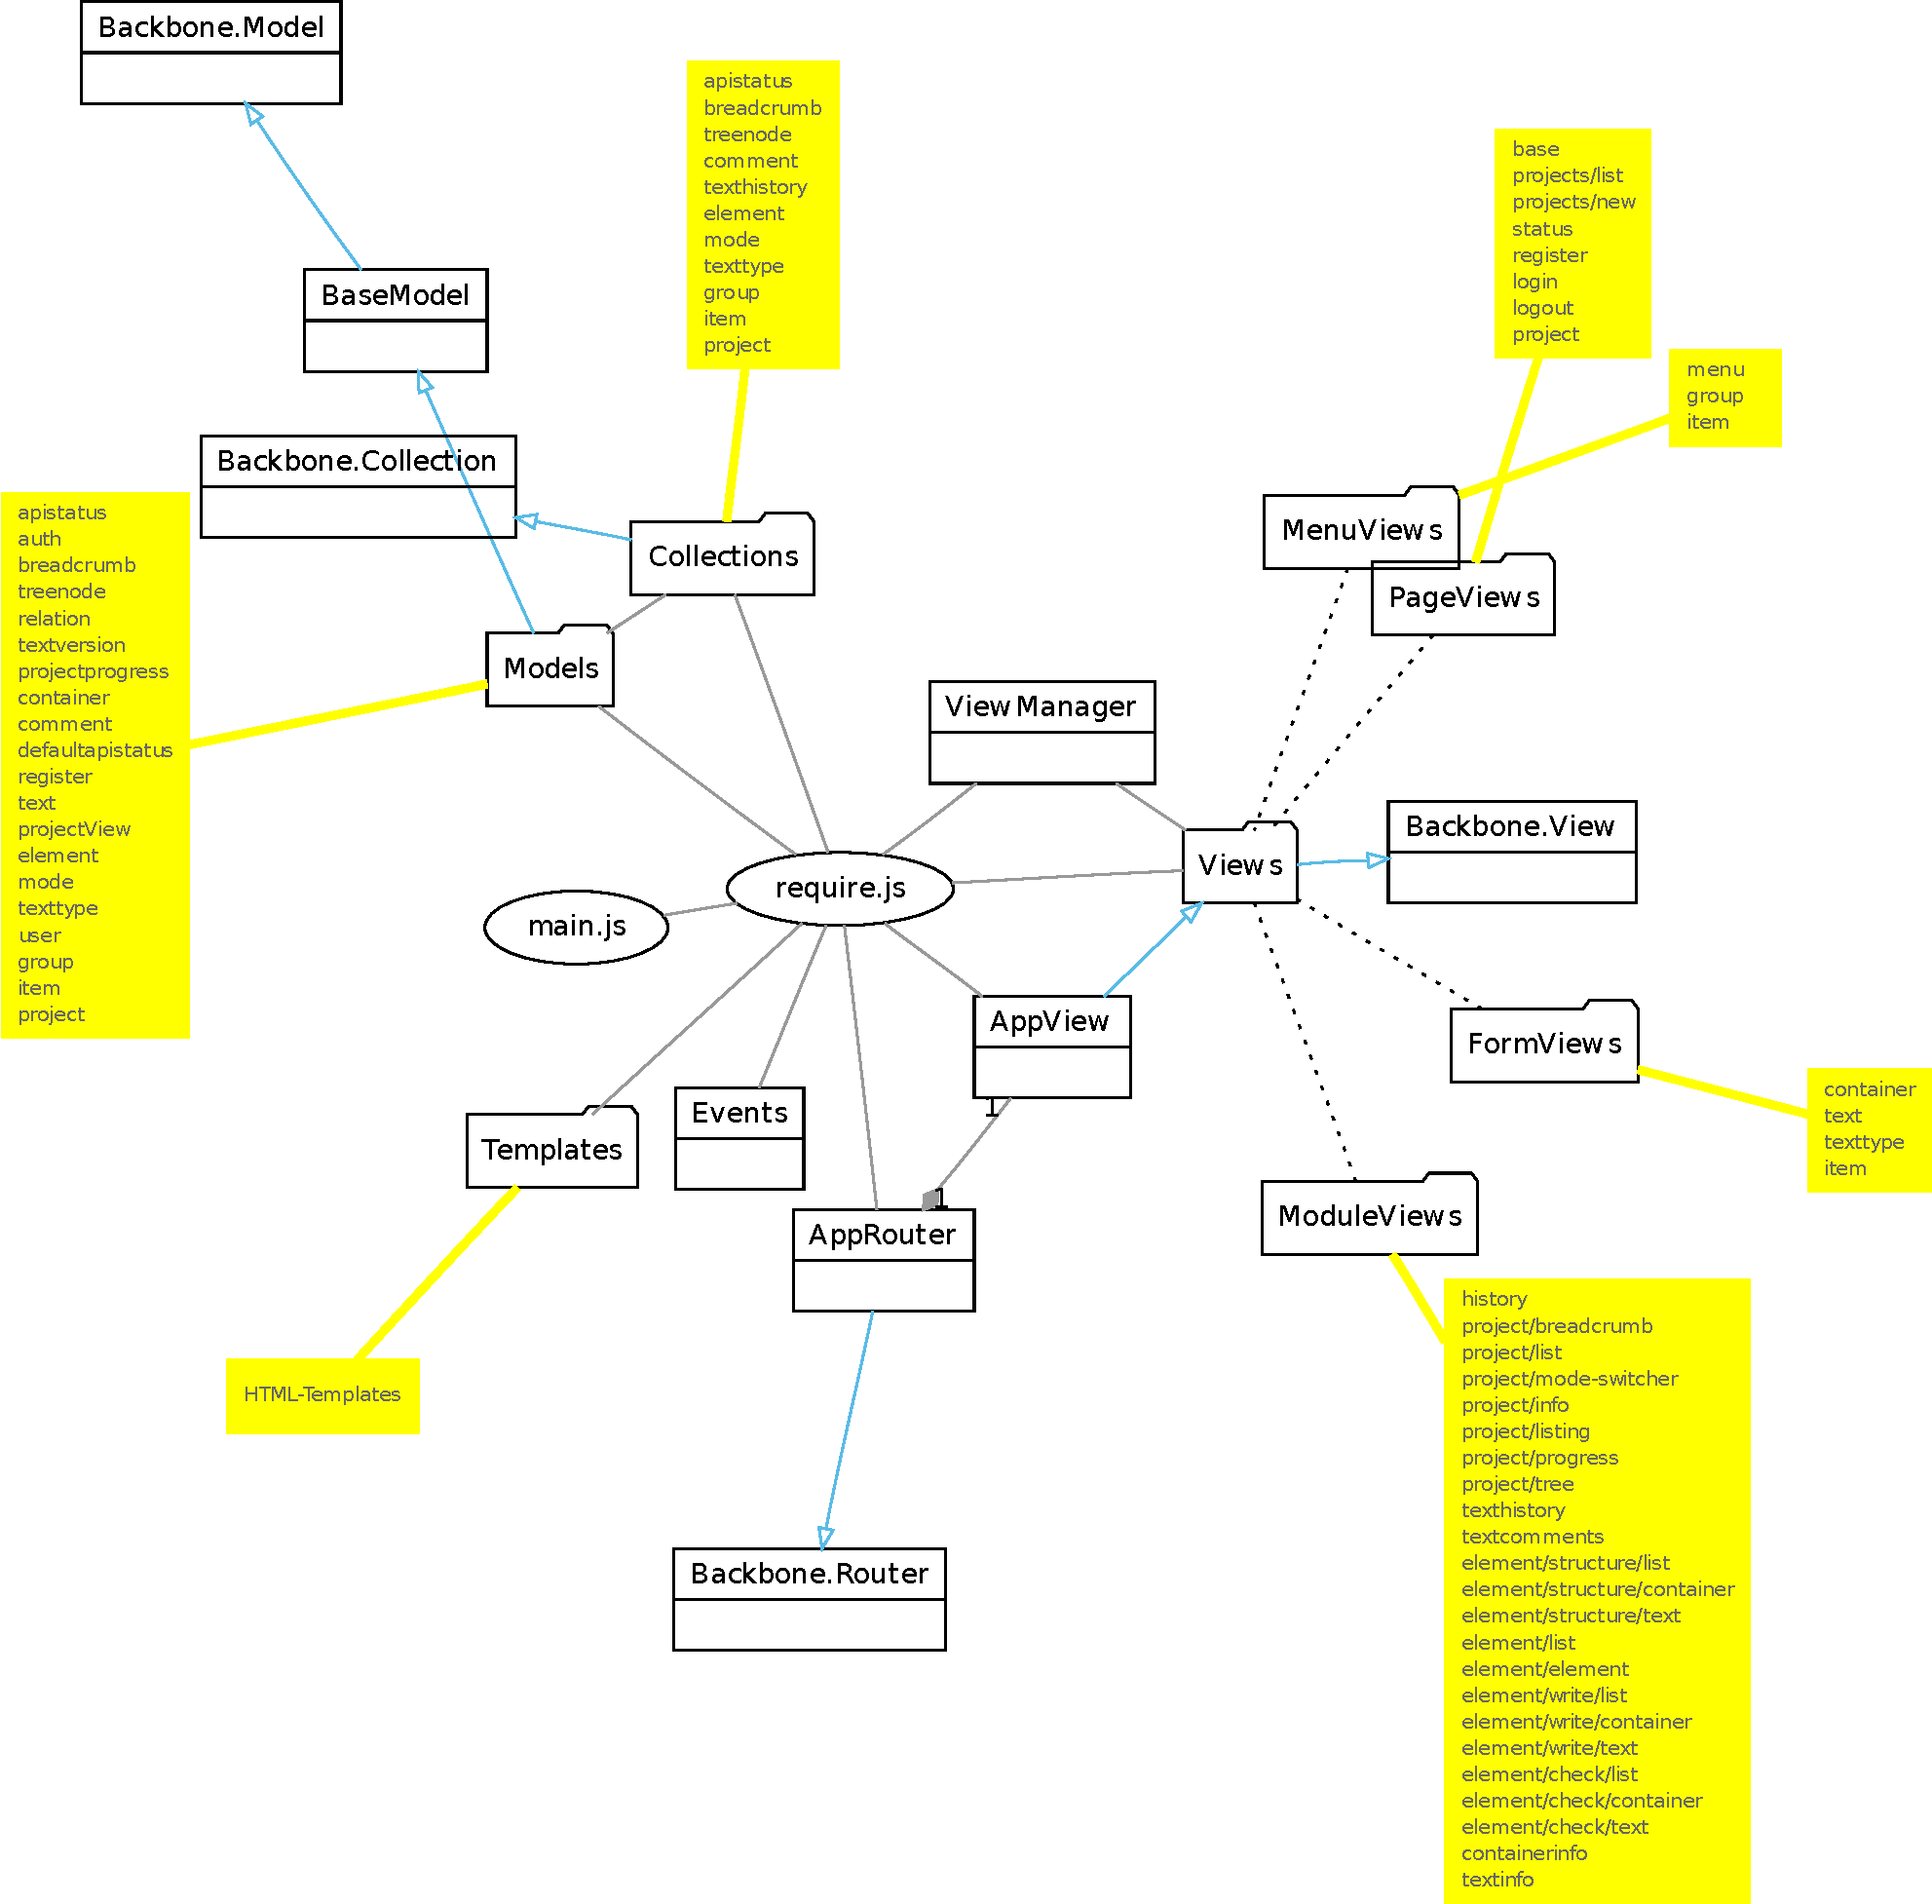
\includegraphics[width=\textwidth]{media/prototyp-gui-klassendiagramm.pdf}
\captionof{figure}{GUI-Klassendiagramm des Prototyps}\label{chart:prototyp-gui-klassendiagramm}
\end{center}

Abbildung \ref{chart:prototyp-gui-klassendiagramm} zeigt das Klassendiagramm der browserbasierten Anwendung. Zentraler Einstiegspunkt ist die JavaScript-Datei \texttt{main.js}, die die Anwendung initialisiert. Dazu lädt sie mithilfe von \texttt{require.js} die notwendigen Komponenten. Dabei handelt es sich zum einen um die \texttt{AppView}, die grundlegende Zustände der Anwendung verwaltet und den \texttt{AppRouter}, der je nach aktueller Route die jeweilige \texttt{PageView} initialisiert und anzeigt. Die \texttt{PageViews} erzeugen danach wiederum eigenständig die von ihnen benötigten Ansichten (\texttt{ModuleViews}, \texttt{MenuViews} und \texttt{FormViews}) und laden die dafür benötigten Daten mithilfe der \texttt{Models} und \texttt{Collections} -- in \trademark{Backbone.js} sind \emph{Views} eigentlich Controller, eine Trennung zwischen Darstellungslogik und Businesslogik ist nicht vorgesehen. Den HTML-Quellcode zur Darstellung laden die Views ebenfalls selbständig aus den \texttt{Templates} nach. Abhängigkeiten wie JavaScript-Objekte und Templates werden dabei zentral von \trademark{require.js} bereitgestellt, das damit die Aufgabe eines Dependency-Injection-Containers (DI-Container) übernimmt und praktisch auch so verwendet werden kann.

Die Kommunikation mit der API wird durch die \trademark{Backbone.js}-Klassen \texttt{Backbone.Model} und \texttt{Backbone.Collection} abstrahiert, die RESTful-APIs ansprechen können, die dem CRUD-Paradigma entsprechen. Siehe dazu die Beschreibung der API-Implementierung in Abschnitt \ref{l:api-implementierung} · S.\pageref{l:api-implementierung}.

\secbar

Das browserbasierte GUI ist zwar eine eigenständige Anwendung, ohne einen Anwendungsserver lässt sich hiermit jedoch nicht arbeiten, da die GUI lediglich zum Darstellen und Modifizieren von Daten verwendet wird. Die Persistenz und vor allem die Sicherung von Datenzugriffen, Berechtigungen, sowie viele weitere Funktionen werden im Anwendungsserver implementiert, der im nächsten Abschnitt beschrieben wird.

\pagebreak

\subsection{Entwurf des Anwendungsservers}\label{l:entwurf-server}

In diesem Abschnitt werden die in Abbildung~\ref{chart:komponenten} · S.\pageref{chart:komponenten} grau eingefärbten Komponenten des Anwendungsservers beschrieben.

\subsubsection{API, Cronjobs, CLI, …}

In der API-Komponente, die als RESTful-API implementiert ist, sind über eine Rou"-ting-Ta"-bel"-le alle Controller registriert. Da das System mit einer vollständigen Abdeckung aller Operationen durch API-Endpunkte implementiert ist, wird diese auch für lokal ausgeführte Scripte wie z.B. Cronjobs oder CLIs verwendet. Dies ermöglicht eine saubere Trennung, auch für administrative Aufgaben, und verhindert, dass Sonderfälle oder Workarounds für bestimmte Aufgaben kultiviert werden.

\subsubsection{Dependency-Injection-Container}

Die einzelnen Komponenten des Anwendungsservers sind nach dem Prinzip der losen Kopplung verbunden (vgl.~\cite[S.62]{hn-web20}). Hierzu werden die einzelnen Komponenten als Services in einem DI-Container registriert und von diesem instanziiert. Alle Komponenten können auf den DI-Container zugreifen und dort andere Komponenten anfordern. Der DI-Container übernimmt, wie der Name schon sagt, auch die Aufgabe Abhängigkeiten der einzelnen Komponenten bereitzustellen. Ein so aufgebautes System, bei dem konkrete Instanzen nicht mehr an der Stelle erzeugt werden, an der sie verwendet werden, sondern von außen \typoquotes{hereingereicht} werden, ist leicht zu modifizieren und vor allem leicht zu testen, da sich Abhängigkeiten für Tests leicht durch Mock-Objekte austauschen lassen (vgl.~\cite[Kap.2]{freeman2009growing}).

\subsubsection{Controller}

Zentrale Komponente bilden die Controller. Hier ist die Business-Logik der Anwendung implementiert. Die einzelnen Operationen sind in verschiedenen Controllern implementiert, so ist das System leicht erweiter- und wartbar. Die Controller werden von der API-Komponente entsprechend den Routen instanziiert, für die sie registriert sind. Controller haben über den DI-Container Zugriff auf alle Teile des Systems und erzeugen die Antwort auf eine Anfrage, die mit der API-Komponente an den Client zurückgeschickt wird.

\subsubsection{Models}

Zu den Kern-Komponenten gehören auch die Models. Diese können ohne den DI-Container direkt von den jeweiligen Komponenten instanziiert werden, da sie reine Datenobjekt sind und weder Logik enthalten, noch von anderen Komponenten abhängig sind. Siehe hierzu auch das Domänenmodell auf S.\pageref{l:domänenmodell}.

\subsubsection{Persistenz, ORM}

Mit dieser Komponente werden die innerhalb der Anwendung erzeugten Daten persistiert. Mithilfe eines Object-Relational-Mappers (ORM) werden die Domänendaten, die durch die Models ausgedrückt werden, in relationale Daten umgewandelt, sofern zur Datenspeicherung ein relationales Datenbanksystem (RDBMS) verwendet wird. Wird hier eine nicht-relationale Datenbank (Dokumentendatenbank, Key-Value-Store) verwendet, kann der ORM entfallen bzw. wird durch ein entsprechende Komponente ersetzt.

\subsubsection{Import/Export \& Benachrichtigung}

\begin{center}
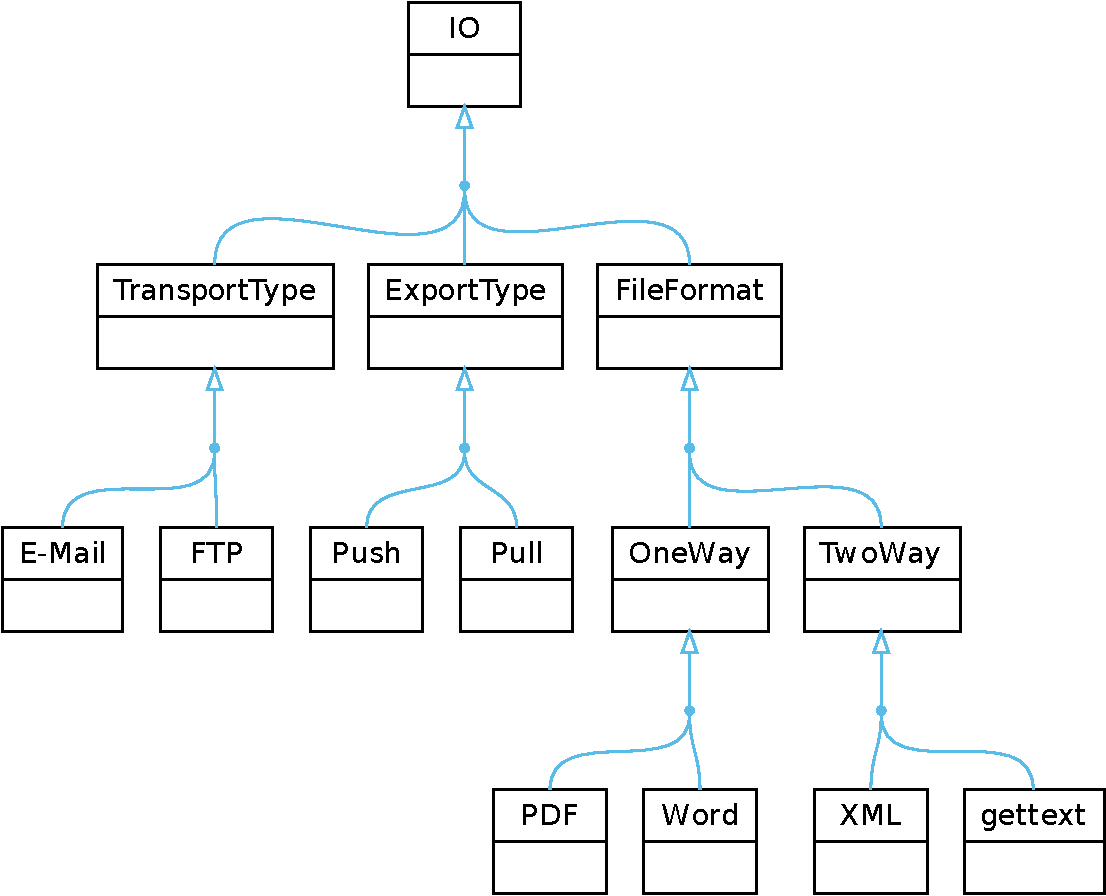
\includegraphics[width=0.75\textwidth]{media/io.pdf}
\captionof{figure}{I/O-Komponente}\label{chart:io}
\end{center}

Diese Komponente ist für den Import von Daten aus verschiedenen Formaten in das interne Repräsentationsmodell und den umgekehrten Export zuständig. Die Komponente ist unterteilt in drei Bereiche für die Implementierungen des Transportwegs (z.B. \emph{E-Mail} oder \emph{FTP}), der Art des Ex- oder Importes (synchron, asynchron bzw. \emph{Push} oder \emph{Pull}) und das Dateiformat (vgl.~Abb.~\ref{chart:io}). Aus diesen drei Teilen lassen sich beliebige Kombinationen erstellen. Beispiele sind synchrone Exporte, wie den Download eines Exports über die Schnittstelle oder asynchrone Exporte, z.B. den Upload auf einen FTP-Server. Benachrichtigungen sind ebenfalls in dieser Komponente implementiert. Eine Benachrichtigung ist z.B. ein asynchroner Export via E-Mail, wobei keine Daten exportiert werden, sondern z.B. nur die Informationen zu einem Ereignis.

\subsubsection{Jobs}

Zeitaufwändige und wiederkehrende Operationen, wie z.B. der Datenimport oder das Versenden von Benachrichtigungen, werden mithilfe von Jobs verarbeitet. Die Informationen zu einem Job werden in die Message-Queue eines Job-Server eingestellt und dort durch registrierte Job-Runner verarbeitet.

\subsubsection{Workflow}

In der Workflow-Komponente sind die Funktionen zur Definition und Ablaufsteuerung von komplexeren Workflows implementiert.

\subsubsection{Service-Adapter}

Über Service-Adapter werden externe Dienste oder andere Softwarekomponenten angebunden, die bestimmte Funktionen für die Anwendung zur Verfügung stellen, z.B. Wörterbücher, Datei-Konverter usw.

\secbar

Die in diesem Abschnitt vorgestellten Komponenten bilden gemeinsam ein umfangreiches, komplexes System, mit dem sich alle Anforderungen abbilden lassen. Der im nächsten Abschnitt beschriebene Prototyp verwendet aufgrund seines sehr überschaubaren Funktionsumfangs nur einen Teil der genannten Komponenten. Es wird jedoch darauf geachtet, die Implementierung möglichst nahe an dieser Vorlage zu realisieren.

\pagebreak

\subsection{Implementierung des Anwendungsservers}\label{l:implementierung-server}

Für den Prototyp wurde das PHP-Framework \trademark{Symfony2}\footnote{\url{http://symfony.com/}} eingesetzt, das von sich aus bereits viele Anforderungen des vorangegangenen Abschnitts erfüllt. 

\subsubsection{Kern-System}

Da im Kern jeder Web-Anwendung HTTP-Anfragen beantwortet werden, überträgt \trademark{Symfony2} dieses Paradigma auf die Art und Weise, wie im Framework Anfragen verarbeitet werden: mithilfe einer Routen-Konfiguration werden Controller für bestimmt Pfade in der Anfrage-URL registriert und dann bei Bedarf vom Framework automatisch instanziert und aufgerufen. Das folgende Listing zeigt dies am Beispiel des \texttt{LoginControllers}, in dem die Methode \texttt{loginAction} aufgerufen wird, wenn der Pfad \texttt{\/login} lautet und die HTTP-Methode der Anfrage \texttt{POST} ist.

\begin{samepage}
\begin{verbatim}
class LoginController extends Base {
    /**
     * @Route("/login", requirements={"_method":"POST"})
     */
    public function loginAction() { … }
}
\end{verbatim}
\end{samepage}

Die Controller schreiben ihre Antwort in ein Objekt, das vom Framework als Antwort gesendet wird. 

Oberstes Prinzip bei der Entwicklung des Frameworks war die Modularisierung und die Wiederverwendbarkeit, so sind alle Komponenten ohne harte Abhängigkeiten mithilfe eines DI-Containers verbunden. Dadurch sind \trademark{Symfony2}-Anwendungen leicht zu warten und auch zu testen, entsprechende Unit-Testing-Komponenten werden bereits mitgeliefert.

\subsubsection{API}\label{l:api-implementierung}

Die API wurde RESTful implementiert und deckt alle Funktionen des Anwendungsservers ab. Sie folgt dem CRUD-Paradigma und unterstützt dementsprechend die jeweiligen Methoden: \texttt{POST} zum Erzeugen von Objekten (CREATE), \texttt{GET} zum Lesen von Objekten (READ), \texttt{PUT} zum Aktualisieren bestehender Objekte (UPDATE) und \texttt{DELETE} zum Löschen von Objekten. Generell werden Daten innerhalb der Anfragen als JSON-Objekte kodiert, URL-Parameter oder eine Kombination von beidem sind ebenfalls zulässig. Eine Aufstellung aller implementierten API-Endpunkte findet sich in Anhang \ref{l:api-endpoints} · S.\pageref{l:api-endpoints}.

Die ausgelieferten JSON-Objekte enthalten Zusatzinformationen zum Kontext und zu Relationen, wie in Abschnitt \ref{l:anbindung-gui} · S.\pageref{l:anbindung-gui} beschrieben. 

\begin{samepage}
\begin{verbatim}
{   "@context":"http://jsonld.retext.it/Container",
    "@id":"/api/container/4fdf26e7820b905118000001",
    "@relations":[
        {
            "@context":"http://coderbyheart.de/jsonld/Relation",
            "relatedcontext":"http://jsonld.retext.it/Project",
            "href":"/api/project/4fdf26e7820b905118000000",
            "list":false
        },
        {
            "@context":"http://coderbyheart.de/jsonld/Relation",
            "relatedcontext":"http://jsonld.retext.it/Element",
            "role":"http://jsonld.retext.it/ontology/child",
            "href":"/api/element?parent=4fdf26e7820b905118000001",
            "list":true
        },
        …
    ],
    "id": "4fdf26e7820b905118000001",
    "name": "Abschnitt 1",
    … }
\end{verbatim}

Dieses Listing zeigt als Beispiel das JSON-Objekt eines Containers. In der \texttt{@relations}-Liste ist der Verweis auf das Eltern-Element enthalten, aber auch auf die Liste mit untergeordneten Elementen dieses Containers. Im Client werden die Relationen je nach Bedarf durchsucht und die passende ausgewählt, sofern weitere Daten benötigt werden. Die jeweilige URL ist in \texttt{href} enthalten, so dass sich im Quellcode des Clients nur wenige hart-kodierte Endpunkte finden.

\end{samepage}

\subsubsection{Persistenz}

\begin{center}
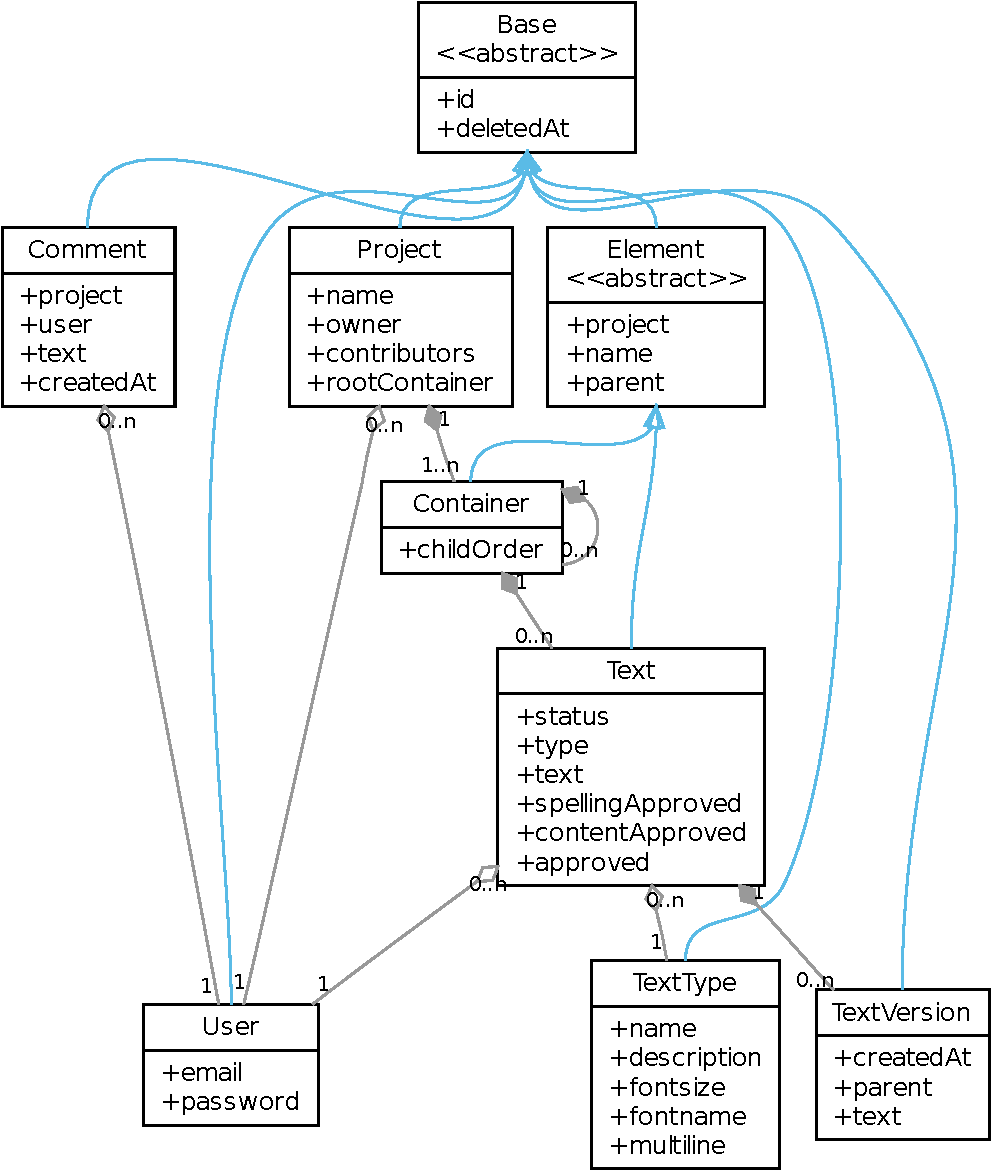
\includegraphics[width=0.65\textwidth]{media/prototyp-persistenz.pdf}
\captionof{figure}{Persistierte Objekte im Prototyp}\label{chart:prototype-persistenz}
\end{center}

Zum Persistieren der Daten kommt \trademark{MongoDB}\footnote{\url{http://www.mongodb.org/}}, eine No-SQL-Datenbank, zum Einsatz. Diese ermöglicht das unkomplizierte Speichern auch komplexer Dokumentenstrukturen als JSON-Objekt. Die Wahl einer nicht-relationen Datenbank bietet den Vorteil, dass aufwändiges Zusammensetzen und Zerlegen von Dokumenten entfallen kann. In der Datenbank werden die in Abbildung \ref{chart:prototype-persistenz} gezeigten Domänenobjekte gespeichert. Dieses Modell ist deutlich einfacher als das in Abschnitt \ref{l:domänenmodell} · S.\pageref{l:domänenmodell} vorgestellte Domänenmodell, da im Prototyp nur wenige, entscheidende Funktionen implementiert wurden. Das Laden- und Speichern ist durch den Einsatz eines Object-Document-Mappers (ODM) für Doctrine 2 und MongoDB\footnote{\url{https://github.com/doctrine/mongodb-odm}} weitestgehend automatisiert. 

\subsubsection{Klassendiagramm}

\begin{center}
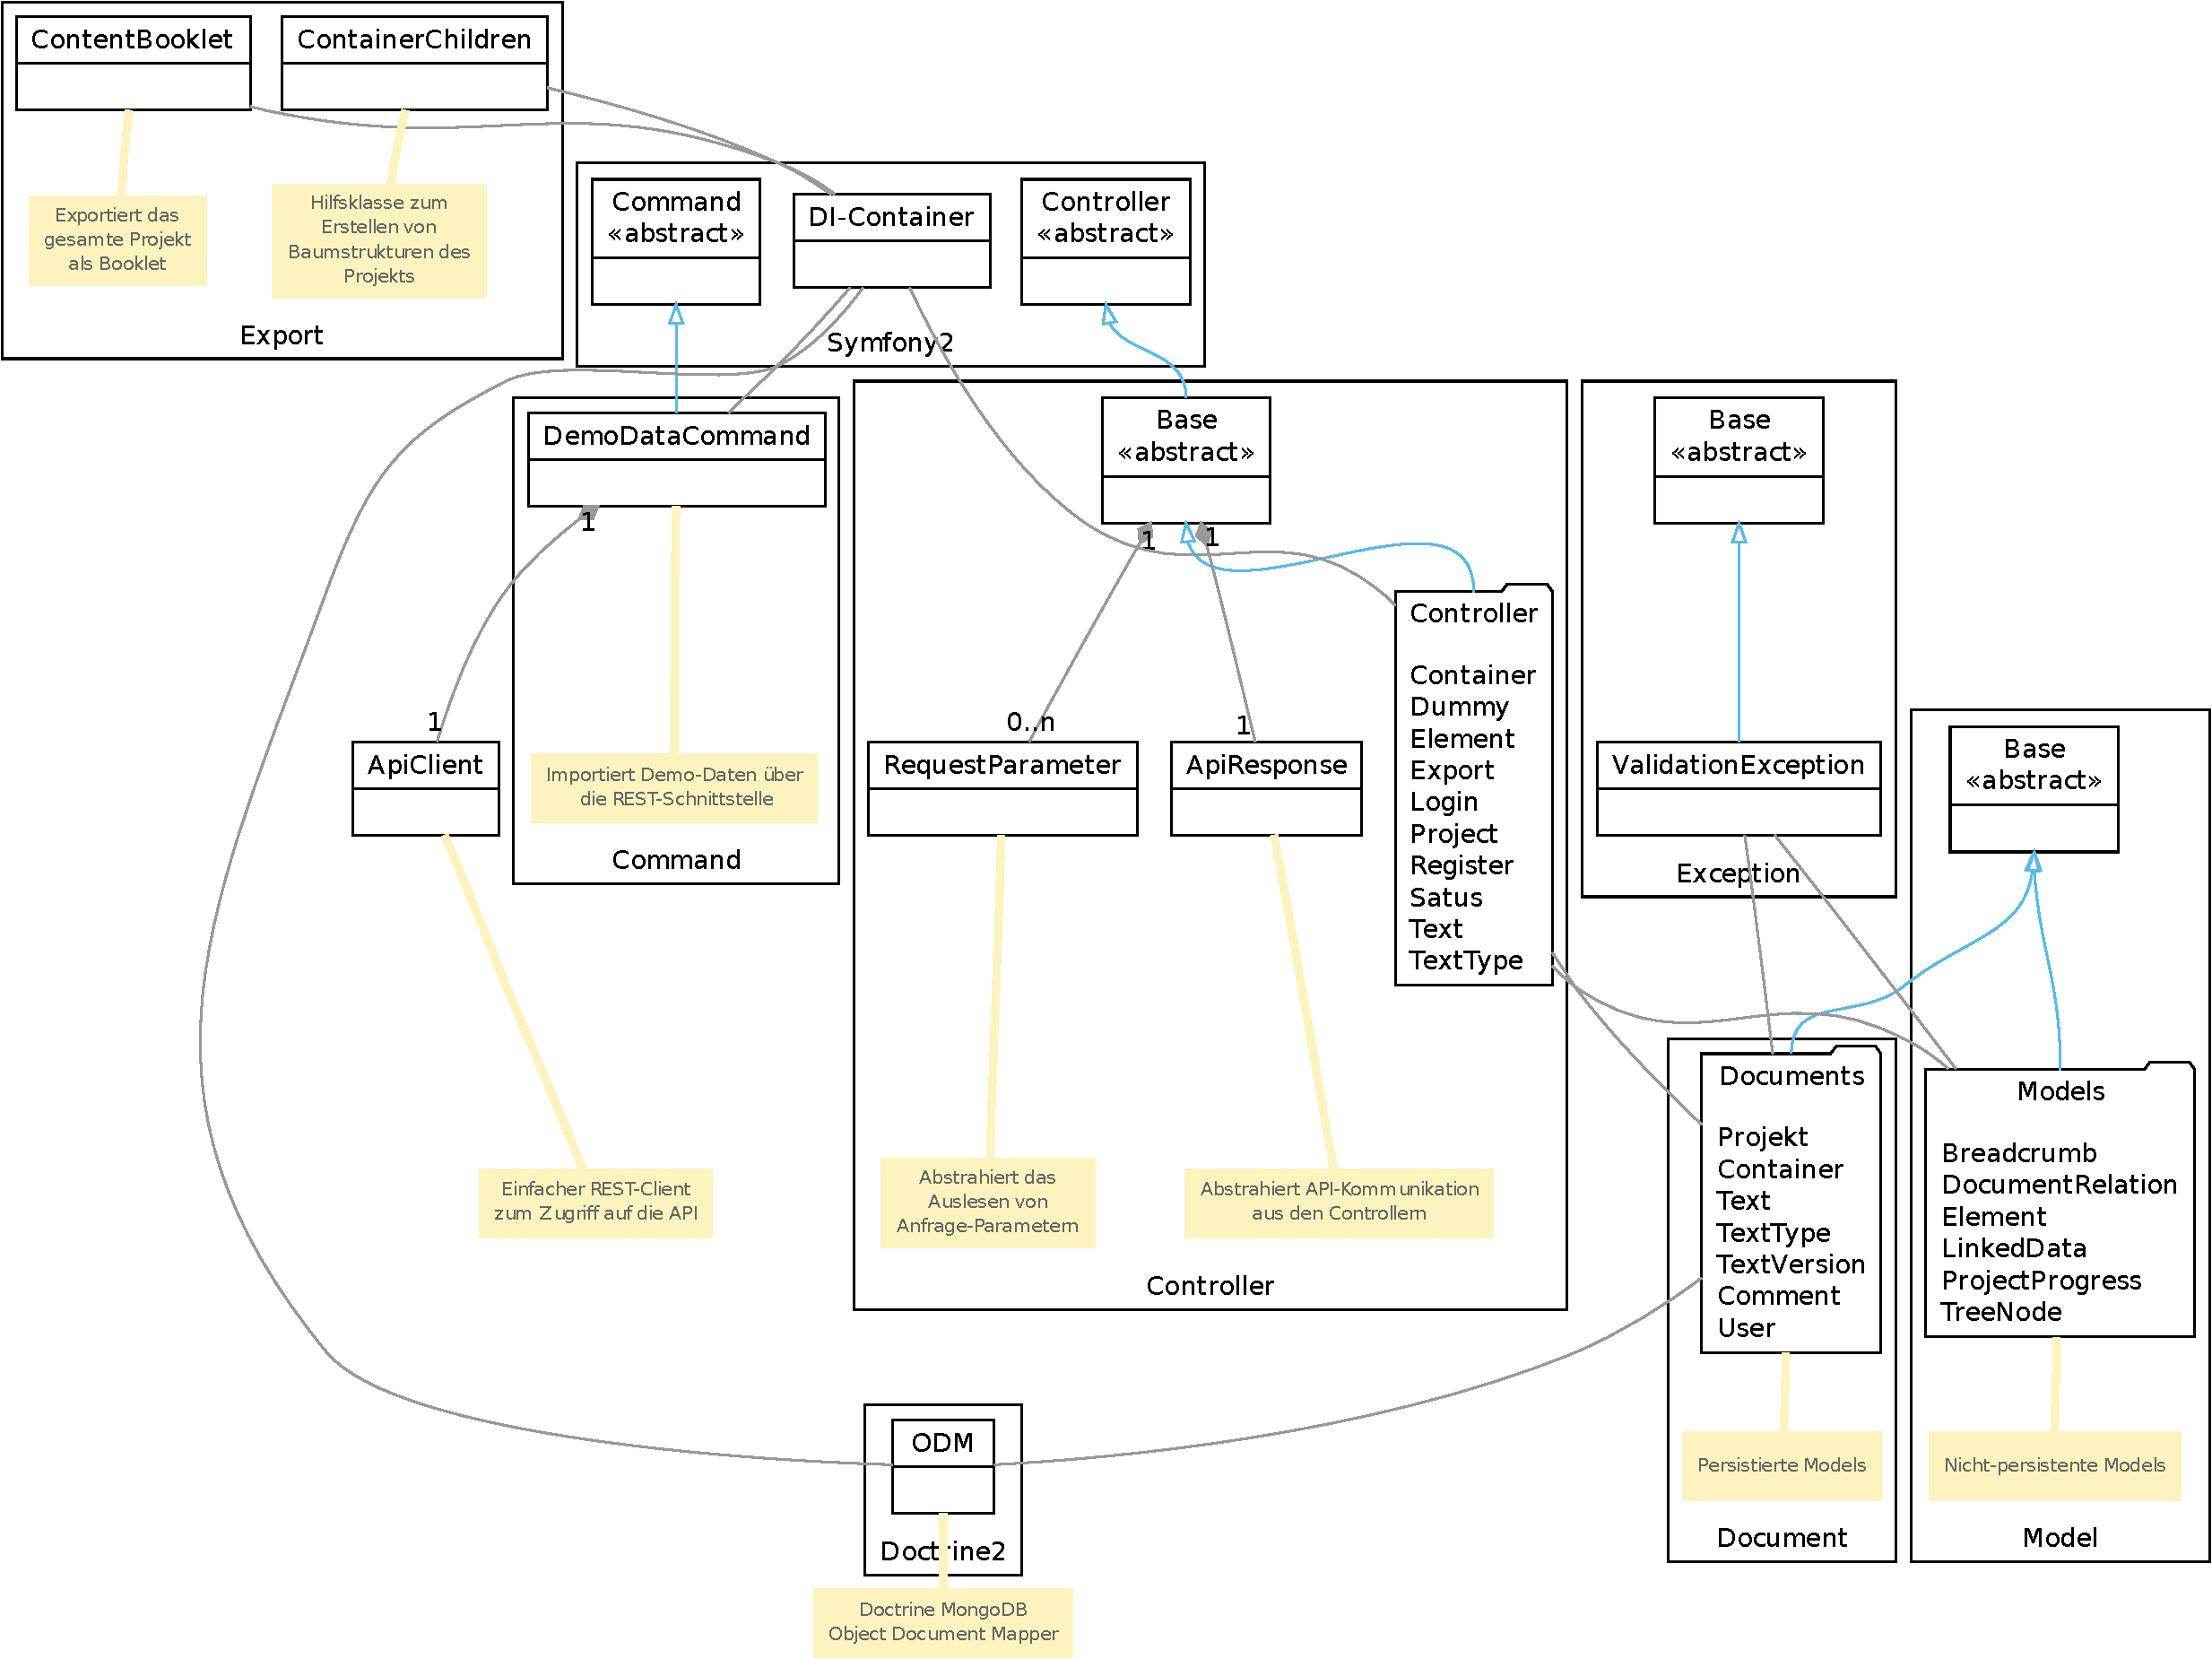
\includegraphics[width=\textwidth]{media/prototyp-klassendiagramm.pdf}
\captionof{figure}{Anwendungsserver-Klassendiagramm des Prototyps}\label{chart:prototyp-klassendiagramm}
\end{center}

Abbildung \ref{chart:prototyp-klassendiagramm} zeigt das Klassendiagramm der Implementierung des Prototyps. Zentrale Komponente ist der DI-Container des Symfony2-Frameworks, dieser instanziert je nach Pfad der Anfrage einen Controller und ruft dort die entsprechende Methode auf. Innerhalb der Controller steht der DI-Container zur Verfügung über den dann z.B. der ODM instanziert werden kann, um Daten aus der Datenbank zu laden. Der ODM verwendet zur Repräsentation der Daten die Klassen des Packages \texttt{Documents}, die Controller können diese selber erzeugen oder bekommen diese als Anfrage-Ergebnisse vom ODM übergeben.

Funktionen, die an mehreren Stellen, oder über unterschiedliche Arten verwendet werden, wurden in eigene Services ausgelagert (\texttt{ContentBooklet} und \texttt{ContainerChildren}). Diese werden zum einen innerhalb der Controller verwendet, können aber auch über das CLI gestartet werden. 

\trademark{Symfony2} stellt eine einfache Möglichkeit zum Erstellen vom Operationen über die Kommandozeile zur Verfügung. Im Prototyp wurde das Anlegen von Demo-Projekt-Daten mithilfe dieser Möglichkeit realisiert. Das \texttt{DemoDataCommand} wird von der Konsole aus gestartet und verwendet den \texttt{ApiClient}, um über HTTP mit der Schnittstelle des Anwendungsservers zu kommunizieren.

\secbar

Die Implementierung eines Prototyps dient zur Verifizierung eines Entwurfs; im folgenden Abschnitt wird der Prototyp in einem realitätsnahen Szenario begutachtet.

\pagebreak

\subsection{Implementierter Workflow am Beispiel des Studiengangsflyers}

Die in den vorangegangenen Abschnitten vorgestellte Implementierung des Prototyps wird anhand eines realen Projekts auf ihre Praxistauglichkeit hin überprüft. Es handelt sich dabei um die einmal im Jahr erscheinende Informationsbroschüre des Studienganges Medieninformatik an der Hochschule RheinMain. Die Broschüre des Wintersemesters 2011/2012 hat einen Umfang von 28 Seiten zuzüglich Titel und Rückseite. In ihr findet sich das Grußwort des Studiengangsleiters, eine Kurzinfo über den Studiengang, das Studienprogramm mit Informationen zum Verlauf des Studiums, ein Terminkalender, Informationen zu Einrichtungen des Fachbereiches, eine Liste mit Personen im Fachbereich, sowie eine Umgebungskarte und ein Gebäudeplan. Die Broschüre wird von den Mitarbeitern des Fachbereiches selber erstellt.

\bigskip

Mit dem Prototyp ist es möglich, den Flyer als Projekt anzulegen. Im nächsten Schritt wird die Struktur des Flyers festgelegt. Die Anwendung unterscheidet dazu zwischen Containern und Textbausteinen. Container sind rein strukturelle Elemente, die wiederum weitere Container und Textbausteine enthalten können. Für den Flyer bietet es sich an, einzelne Kapitel (Titel, Vorwort, Kurzinfo, Termin \& Öffnungszeiten, Personen, Orientierung) als Container auf oberster Ebene anzulegen und darunter jeweils weitere Unterteilungen nach Abschnitten vorzunehmen. Innerhalb dieser Abschnitte werden dann die einzelnen Textbausteine definiert. Zu den Textbausteinen können auch Zusatzinformationen zum Text-Typ (Schriftart, Schriftgröße, ein- oder mehrzeilig) hinterlegt werden. Die Elemente lassen sich mittels Drag\&Drop in der Reihenfolge anpassen.

Sobald die Bestandteile des Produkts angelegt wurden kann parallel bereits mit der Erstellung der Texte begonnen werden. Diese können in den jeweiligen Bausteinen je nach Typ als ein- oder mehrzeiliger Text hinterlegt werden. Änderungen an den Inhalten werden gespeichert und sind als Änderungsverlauf abrufbar. Über eine Kommentarfunktion ist der Austausch über die Texte innerhalb der Anwendung möglich. 

In der Ansicht zur Freigabe können die einzelnen Texte überprüft und abgenommen werden. Es wird zwischen den Status für Rechtschreibung, Inhalt und der allgemeinen Freigabe unterschieden. Bei Statusänderungen wird automatisch ein Kommentar erzeugt, das beim Ablehnen durch den Benutzer mit Zusatzinformationen versehen werden kann. Die einzelnen Status werden aggregiert und als Gesamt-Status für das gesamte Projekt, sowie zur Übersicht und zum schnellen Zugriff in der Projektstruktur angezeigt.

Als Beispiel für die Verwendung der Projektdaten in externen Systemen lässt sich das Projekt als \emph{Content-Booklet} im HTML- oder PDF-Format exportieren. Dieses Dokument enthält alle Information in strukturierter Form, so wie sie im System angelegt wurden und listet neben den Texten auch die jeweiligen Zusatzinformationen auf. Mithilfe des \emph{Content-Booklet} können Produzenten einfach mit der neuesten Version der Texte für das Produkt versorgt werden und es liefert einen Überblick über alle Bestandteile des Produkts. Ein Ausschnitt aus diesem Booklet findet sich in Anhang \ref{l:booklet} · S.\pageref{l:booklet}.

\secbar

Der Prototyp ist in der Lage, bereits mit diesem einfachen Funktionsumfang einen praktischen Mehrwehrt für ein Produkt wie den Studiengangsflyer zu bieten. Die Texte können gemeinsam und nachvollziehbar erfasst werden, der Export als \emph{Content-Booklet} kann verschiedenen Mitarbeitern bei der Erstellung des fertigen Produkts konkrete Hilfestellung bieten.

\pagebreak

\subsection{Zusammenfassung}

In diesem Kapitel wurde das zentrale System der Anwendung, bestehend aus Anwendungsserver und browserbasiertem GUI entworfen und beschrieben. Der Aufbau des Anwendungsserver mithilfe einer lose gekoppelten Architektur ermöglicht einfache Erweiterbarkeit und Wartung. Das browserbasierte GUI ist als JavaScript-MVC-Anwendung entworfen, die über eine RESTful-API mit dem Anwendungsserver kommuniziert. Die wichtigsten Ansichten des GUIs wurden mithilfe von Wireframes beschrieben. 

Der Entwurf wurde mithilfe einer prototypischen Implementierung, in der die wichtigsten Abläufe abgebildet werden, anhand eines realen Projekts überprüft. Dabei wurde gezeigt, dass sich die vorgeschlagenen Prinzipien, in der Darstellung wie in der Implementierung mit aktuell verfügbaren Technologien problemlos umsetzen lassen. Zudem wurde gezeigt, dass das Konzept der Trennung zwischen Anwendungsserver und GUI keine negativen Auswirkungen auf die Verwendbarkeit einer Anwendung hat. Für die Realisierung weiterer Funktionen im Sinne des Entwurfes sind keine Hindernisse aufgetreten.

\secbar

Der in diesem Kapitel vorgestellte Entwurf liefert damit die Basis für die mögliche Entwicklung einer vollwertigen Lösung und bietet für einzelne Bestandteile bereits mögliche Technologieempfehlungen.

\pagebreak


\section{Implementierung eines Prototypen}\label{l:implementierung}

\subsection{Grundüberlegung}

Content-Management-Systeme bzw. Redaktionssystem können einen Teil der Aufgabe abbilden, sind aber i.d.R. ungeeignet (z.B. kein Workflow), keine Context-Informationen hinterlegbar.

\subsection{Abgrenzung}
\subsection{Beschreibung der gewählten Umsetzung, Komponenten}

\subsection{Anwendung der Umsetzung am Beispiel des Studiengangsflyers}

Die vorgeschlagene Lösung wird anhand eines realen Projektgs auf ihre praxistauglichkeit hin überprüft. Es handelt sich dabei um die einmal im Jahr erscheinende Informationsbröschüre des Studienganges Medieninformatik an der Hochschule RheinMain. Die Bröschure zu Beginn des Wintersemesters 2011/2012 einen Umfang von 28 Seiten zuzüglich Titel und Rückseite. In ihr findet sich das Grußwort des Studiengangsleiters, eine Kurzinfo über den Studiengang, das Studienprogramm mit Informationen zum Verlauf des Studiums, ein Terminkalender, Informationen zu Einrichtungen des Fachbereiches, eine Liste mit Personen im Fachbereich, sowie eine Umgebungskarte und ein Gebäudeplan. Die Broschüre wird von den Mitarbeitern des Fachbereiches selber erstellt.

\paragraph{Workflow}

Innerhalb der Anwendung wird das Projekt angelegt und die dafür benötigten Textbausteine definiert. Hierbei können detaillierte Angaben zu deren Eigenschaften gemacht werden, z.B. über den Verwendungszweck oder die maximal Länge. Die einzelnen Textbausteine werden bei diesem Vorgang entsprechend dem Aufbau des Endproduktes in eine Reihenfolge gebracht und hierarchisch angeordnet. So wird eine leichte Orientierung und Zuordnung der Text zum Endprodukt möglich. 

Nachdem die benötigten Textbausteine definiert wurden, werden diese durch Texter befüllt. Für Texter stellt die Anwendung Hilfsfunktionen zur Verfügung. Dazu zählen Informationen wie Zeichenlänge und Wortanzahl und Rechtschreibkorrektur mit Wörterbuch.

Sobald die Texte hinterlegt wurden durchlaufen sie die Qualitätskontrolle durch andere Mitarbeiter des Projektes und anschließend den Freigabeprozess beim Kunden. Wurden die Texte freigegeben, können die zusammengestellten Texte in das Endprodukt übernommen werden. 

Alle Vorgänge werden innerhalb der Anwendung protokolliert und sind so für jeden Beteiligten leicht nachvollziehbar. Aufgaben können automatisch aufgrund von Änderungen erzeugt werden, oder von Mitarbeiter angelegt werden. So wird sichergestellt, dass alle Projektmitarbeiter jederzeit über ihre Aufgaben bezüglich der Texte informiert sind, bei Änderungen die verantwortlichen Mitarbeiter informiert werden. Dadurch wird es möglich auch bei Korrekturen in letzter Minute diese Änderungen gezielt und transparent zu übernehmen.

\pagebreak

\section{Fazit}\label{l:fazit}

Diese Bachelor-Thesis hat sich mit der Fragestellung beschäftigt, wie es dazu kommt, dass trotz aller technischer Fortschritte im Bereich der Informationstechnologie bei der Organisation von Texten für Medienprodukte auf Arbeitsweisen zurückgegriffen wird, die inzwischen überholt sein sollten und wie eine bessere Lösung für diese Aufgaben aussehen könnte.

Es wurde gezeigt, dass die gebräuchlichen Werkzeuge, \trademark{Microsoft Word} und \trademark{Excel}, in der alltäglichen Arbeit in Agenturen zu vielerlei Problemen führen, sie aber verwendet werden, weil die Nutzer zum einen deren Gebrauch gewöhnt sind und zum anderen die Werkzeugen scheinbar über alle notwendigen Funktionen für diese Aufgabe verfügen. In einer ausführlichen Analyse wurde diese Annahme jedoch widerlegt und im Einzelnen gezeigt, welche problematischen Auswirkungen der Einsatz monolithischer Dateiformate und dezentraler Speicherung in den komplexen Abläufen in Zusammenhang mit der Erstellung von Medienprodukten haben.

Aufbauend auf dieser Erkenntnis und unter Zuhilfenahme von Personas, die auf Interviews mit zwölf Branchenexperten basieren, wurde eine Lösung konzipiert, die versucht, die genannten Probleme zu beseitigen und den Anforderungen der Personas zu genügen. Hierzu wurde ein zentraler Anwendungsserver vorgeschlagen, auf den mit spezialisierten, an die jeweiligen Bedürfnisse der Benutzer angepassten, GUIs zugegriffen wird. Mit deren Hilfe werden die Texte der Produkte definiert, geschreiben, korrigiert, kontrolliert, freigegeben und veröffentlicht.

Für die wichtigsten Bestandteile der Lösung, den Anwendungsserver und das browserbasierte GUI, wurde die konkrete Architektur entworfen und detaillierte Gestaltungsrichtlinen mithilfe von Wireframes festgelegt.

Zur Validierung des Entwurfs wurde schließlich ein Prototyp umgesetzt, der die wichtigsten Funktionen anhand eines Beispiel-Projektes implementiert. Die Implementierung zeigte, dass das Konzept funktioniert, der Entwurf realisierbar ist und bereits die prototypischen Fassung konkreten Mehrwert bietet.

\secbar

Diese Bachelor-Thesis liefert eine konkrete Empfehlung für die Realisierung einer Anwendung zur Verwalten von Texten für Medienprodukte. Sie orientiert sich dabei an den tatsächlichen Abläufen in Projekten zur Erstellung von Informations- und Kommunikations-Medien und den Bedürfnissen der beteiligten Personen. Die vorgestellte Lösung bietet die Möglichkeit, im Projektverlauf in großem Maße Zeit einzusparen und Fehler zu vermeiden.

\pagebreak

\pagebreak

\bibliography{parts/bibliothek}

\end{document}